\documentclass[a4paper, 11pt]{article}

\usepackage[utf8]{inputenc}
\usepackage[T1]{fontenc}
\usepackage[english]{babel}
\usepackage{enumitem}
\usepackage{stmaryrd}
\SetSymbolFont{stmry}{bold}{U}{stmry}{m}{n}
\usepackage{amsthm, amsmath, amssymb, amsfonts, mathtools, mathrsfs}
\usepackage{graphicx, calc}
\usepackage{empheq}
\usepackage{geometry}
\geometry{a4paper, left = 20mm, right = 20mm, top = 30mm, bottom = 30mm}
\usepackage{xspace}
\usepackage{relsize}
\usepackage{fancyhdr}
\usepackage{pdflscape}
\usepackage{csquotes}
\usepackage{titling}
\usepackage{accents}
\usepackage[labelfont=bf,labelsep=period]{caption}
\usepackage{subcaption}
\usepackage{placeins} % FloatBarrier
\usepackage{physics}
\usepackage{tikz,tikz-3dplot}
\usetikzlibrary{patterns,decorations,decorations.pathreplacing,decorations.markings,positioning,calc}
\usepackage{lmodern}
\usepackage{xcolor}
\usepackage{booktabs}
\usepackage{chngcntr}
\usepackage{algorithm}
\usepackage{algorithmicx}
\usepackage{algpseudocode}
\usepackage[sorting=none, style=numeric]{biblatex}
\addbibresource{references.bib}


\usepackage{hyperref}
\hypersetup{
	colorlinks,
	citecolor=green,
	filecolor=black,
	linkcolor=blue,
	urlcolor=blue
}


\pagestyle{fancy}
\fancyhf{}
\setlength{\headheight}{30pt}
\lhead{Numerical Solution of the Convection--Diffusion Equations}
\rhead{ESEIAAT 2020--2021}
\cfoot{\thepage}

\setlength{\parskip}{0.2cm}%

% Comandos
\newcommand{\n}{\mathbb{N}}
\newcommand{\z}{\mathbb{Z}}
\newcommand{\q}{\mathbb{Q}}
\renewcommand{\real}{\mathbb{R}}
\newcommand{\cplex}{\mathbb{C}}
\renewcommand{\k}{\mathbb{K}}
\newcommand{\car}[1]{\mathrm{char}\left(#1\right)}
\newcommand{\class}[1]{\overline{#1}}
\newcommand{\mcd}[1]{\mathrm{mcd}{#1}}
\renewcommand{\mod}[1]{\ (\mathrm{mod}\ #1)}
\newcommand{\fractions}[1]{\mathrm{Fr}(#1)}
\renewcommand{\gcd}[1]{\mathrm{mcd} #1}
\newcommand{\mcm}[1]{\mathrm{mcm} #1}
\newcommand{\conj}[1]{\overline{#1}}
\newcommand{\prob}[1]{p \left( #1 \right)}
\newcommand{\esp}[1]{\mathbb{E} \left[ #1 \right]}
\newcommand{\scr}[2]{\left\langle #1, #2 \right\rangle}
\newcommand{\Int}{\int\limits}
\newcommand{\id}{\mathrm{Id}}
\newcommand{\lt}[1]{\mathrm{LT}(#1)}
\newcommand{\lc}[1]{\mathrm{LC}(#1)}

\newcommand{\divides}{\mid}
\newcommand{\notdivides}{\nmid}
\newcommand{\MATLAB}{\textsc{Matlab}\xspace}
\newcommand{\CC}{C\nolinebreak[4]\hspace{-.05em}\raisebox{.4ex}{\relsize{-3}{\textbf{++}}} }

\newcommand{\separation}{
	\begin{center}
		\rule{\textwidth-20pt}{1pt}
	\end{center}
}

% Control volume and surface commands
\newcommand{\cv}[1]{\mathcal{V}_{#1}}
\newcommand{\cs}[1]{\mathcal{S}_{#1}}
\newcommand{\cvt}{{\mathcal{V}(t)}} 
\newcommand{\cst}{{\mathcal{S}(t)}} 

% Adimensional numbers
\newcommand{\peclet}{\mathrm{Pe}}

\newcommand{\maxf}[2]{\left\llbracket #1, #2 \right\rrbracket}

% Comandos grupos
\newcommand{\generated}[1]{\langle #1 \rangle}



% Conjunto vacío
\let\oldemptyset\emptyset
\let\emptyset\varnothing

% Imagen
\DeclareMathOperator{\image}{Im}


% Abreviaciones
\newcommand*{\eg}{e.g.\@\xspace}
\newcommand*{\ie}{i.e.\@\xspace}


% Conjunto cociente
\newcommand{\quotient}[2]{{\raisebox{.2em}{$#1$}\left/\raisebox{-.2em}{$#2$}\right.}}

% Numerales romanos en el texto
\makeatletter
\newcommand*{\rom}[1]{\expandafter\@slowromancap\romannumeral #1@}
\makeatother


%\DeclarePairedDelimiter\abs{\lvert}{\rvert} 		% abs
\DeclarePairedDelimiter\ceil{\lceil}{\rceil}		% ceil
\DeclarePairedDelimiter\floor{\lfloor}{\rfloor}		% floor

% Enumerate definición
\newlist{enumeratedef}{enumerate}{3}
\setlist[enumeratedef]{label=(\roman*),topsep=0pt}

% Enumerate proposición
\newlist{enumerateprop}{enumerate}{3}
\setlist[enumerateprop]{label=(\arabic*),topsep=0pt}

% Enumerate ejemplo
\newlist{enumeratex}{enumerate}{3}
\setlist[enumeratex]{label=\arabic*.,topsep=0pt}

% Enumerate ejercicio
\newlist{enumeratexercise}{enumerate}{3}
\setlist[enumeratexercise]{label=(\alph*),topsep=0pt}

\makeatletter
\renewenvironment{proof}[1][\proofname]{\par
	\vspace{-\topsep}% remove the space after the theorem
	\pushQED{\qed}%
	\normalfont
	\topsep0pt \partopsep0pt % no space before
	\trivlist
	\item[\hskip\labelsep
	\itshape
	#1\@addpunct{.}]\ignorespaces
}{%
	\popQED\endtrivlist\@endpefalse
	\addvspace{6pt plus 6pt} % some space after
}
\makeatother

% Align images at top of the page when using [ht]
\makeatletter
\setlength{\@fptop}{0pt}
\makeatother


% New colors
\definecolor{nodeColor}{RGB}{62,180,0} 
\definecolor{tempColor}{RGB}{255,0,0} 
\definecolor{meatColor}{RGB}{255,90,90}
\definecolor{greencv}{RGB}{46,204,113}
\definecolor{greenNode}{RGB}{39,174,96}

\definecolor{dofill}{RGB}{130,130,130}
\colorlet{sblue}{blue!70!white}


\newlength{\lside}
\setlength{\lside}{3pt}
\newlength{\alength}
\setlength{\alength}{2pt}

\numberwithin{equation}{section}
\counterwithin{figure}{section}
\counterwithin{table}{section}






\newtheoremstyle{normal}
	{}                % Space above
	{}                % Space below
	{\upshape}        % Theorem body font % (default is "\upshape")
	{}                % Indent amount
	{\bfseries}       % Theorem head font % (default is \mdseries)
	{.}               % Punctuation after theorem head % default: no punctuation
	{ }               % Space after theorem head
	{}                % Theorem head spec
\theoremstyle{normal}

\newtheorem{theorem}{Theorem}[section]
\newtheorem{definition}[theorem]{Definition}
\newtheorem{prop}[theorem]{Proposition}
\newtheorem{lemma}[theorem]{Lemma}
\newtheorem{col}[theorem]{Corollary}
\newtheorem{example}[theorem]{Example}
\newtheorem{obs}[theorem]{Observation}


\newtheorem*{theorem*}{Theorem}
\newtheorem*{definition*}{Definition}
\newtheorem*{prop*}{Proposition}
\newtheorem*{lemma*}{Lemma}
\newtheorem*{col*}{Corollary}
\newtheorem*{example*}{Example}
\newtheorem*{obs*}{Observation}
\newtheorem*{exercise*}{Exercise}
\newtheorem*{notation*}{Notation}





\input{units.tex}

\usepackage{lipsum}

\begin{document}
	
\input{title}
\shipout\null

\tableofcontents
\clearpage	
\section{Introduction}

When we study a fluid under certain hypothesis, its thermophysical properties, namely the density
$(\rho)$, the velocity field $(\vb{v})$, the temperature $(T)$ and the
concentration of a pollutant $(Y_k)$, are governed by the following system of conservation laws:
\begin{gather}
    \pdv{\rho}{t} + \div(\rho \vb{v}) = 0 \label{eq:cont} \\
    \pdv{(\rho \vb{v})}{t} + \div(\rho \vb{v} \otimes \vb{v}) = 
	\div(\mu \grad{\vb{v}}) + 
    \left\{ \div(\vb{\tau - \mu \grad{\vb{v}}}) - \grad{p} + \rho \vb{g} \right\} \label{eq:vel}\\
	\pdv{(\rho T)}{t} + \div(\rho \vb{v} T) = 
	\div(\frac{\lambda}{c_v} \grad{T}) + 
	\left\{ \frac{\vb{\tau} \circ \grad{\vb{v}} - \div{\dot{\vb{q}}^R} - p \div{\vb{v}}}{c_v}\right\} \\
	\pdv{(\rho Y_k)}{t} + \div(\rho \vb{v} Y_k) = 
	\div(\rho D_{km} \grad{Y_k}) + \left\{ \dot{\omega}_k \right\} \label{eq:conc}
\end{gather}
Equation \eqref{eq:cont} is the mass--conservation or continuity equation,
whilst equations \eqref{eq:vel} through \eqref{eq:conc} are known as the
convection--diffusion equations. In this project we study these equations and
their numerical resolution for two special problems.

In section \ref{sec:the_convection_diffusion_equations} we rigorously derive the
continuity and the general convection--diffusion equation. We explain their
numerical resolution and give a solving algorithm in the case of cartesian grid
on a rectangular domain in section \ref{sec:numerical_study}. Finally in
sections \ref{sec:diagonal_flow_case} and \ref{sec:smith_hutton_case} we treat
two steady state problems: the diagonal flow case and the Smith--Hutton case. We
study the analytical solutions of both problems for special values of Péclet's
number, providing existence and uniqueness theorems when possible, and we solve
them numerically in different situations. 




\clearpage	
\section{The convection--diffusion equations}

In this section, a rigorous derivation of the convection--diffusion equations is done. To begin, Reynolds transport theorem is presented as a generalization of Leibniz integral rule and is proved. Next, the distinct conservation laws are derived. Finally a common structure on convection--diffusion equations, which will ease their numeric study, is found.


\subsection{Reynolds transport theorem}

The main result needed to derive the conservation laws of the subsequent subsections, namely, mass, momentum, energy and species conservation, is Reynolds transport theorem. This theorem is a generalization to higher dimensions of Leibniz integral rule:

\begin{theorem}[Leibniz integral rule \cite{kaplan2002advanced}]
	Let $U \subset \real$ be a closed interval and $I = [t_1, t_2]$, and let $a, b \colon I \rightarrow U$ be continuous functions with continuous derivative. Let $f \colon U \times I \rightarrow \real$, $(x,t) \mapsto f(x,t)$ be a continuous function such that $\pdv{f}{t}$ is also continuous. Then for all $t \in I$,
	\begin{equation} \label{eq:leibniz_rule}
		\frac{\dd}{\dd{t}} \int_{a(t)}^{b(t)} f(x,t) \dd{x} = 
		\int_{a(t)}^{b(t)} \pdv{f}{t}(x,t) \dd{x} + f(b(t),t) b'(t) - f(a(t),t) a'(t)
	\end{equation}
\end{theorem}

\noindent
Reynolds transport theorem allows us to compute the left--hand side of \eqref{eq:leibniz_rule} but in the more general context where $f$ is integrated over a bounded smooth control volume $\cv{}(t) \subset \real^m$ which depends upon time. 

\begin{theorem}[Reynolds transport theorem \cite{kundu2008fluid}]
	Let $U \subset \real^m$ be a compact set and let $\cv{}(t)$ be a control volume depending on time such that it is smooth and $\cv{}(t) \subset U$ for all $t \in I = [0, T]$ with $T > 0$. Let $\cs{}(t) = \partial \cv{}(t)$ be the boundary of $\cv{}(t)$ and let $F \in \mathcal{C}^1(U \times I, \real)$ be a scalar field. Then for all $t \in I$,
	\begin{equation} \label{eq:reynolds_transport_theorem}
		\frac{\dd}{\dd{t}} \int_\cvt F(\vb{x}, t) \dd{\vb{x}} = 
		\int_\cvt \frac{\partial F}{\partial t} (\vb{x}, t) \dd{\vb{x}} + 
		\int_\cst F(\vb{x}, t) \vb{b} \vdot \vb{n} \dd{S}
	\end{equation}
	where $\vb{b} \colon \cs{}(t) \rightarrow \real^m$ is the local velocity of the control surface.
\end{theorem}
\begin{proof}
	The moving control volume $\cv{}(t)$ can be seen as the image of an initial region $\cv{}(0)$ by a family of smooth maps $\xi \colon U \times I \subset \real^m \times \real \rightarrow \real^m$, that is to say, $\cv{}(t) = \xi(\cv{}(0),t)$ for all $t \in I$. Moreover, by fixing one time $t$, the mapping $\xi(\cdot, t) \colon \vb{}(0) \rightarrow \vb{}(t)$ can be assumed to be a diffeomorphism. Since $F$ is continuous, we can apply the Change of Variables Theorem taking $\vb{x} = \xi(\vb{x}_0,t)$,
	\begin{equation*}
		\int_\cvt F(\vb{x},t) \dd{\vb{x}} = 
		\int_{\cv{}(0)} F(\xi(\vb{x}_0,t), t) \abs{\det(\frac{\partial \xi}{\partial \vb{x}_0} (\vb{x}_0, t))} \dd{\vb{x}_0}
	\end{equation*}
	where the determinant of the jacobian matrix $\det(\frac{\partial \xi}{\partial \vb{x}_0} (\vb{x}_0, t))$ can be assumed to be positive for small enough $T$, hence the absolute value is dropped. Applying differentiation under the integral sign (Theorem \ref{theo:differentiation_under_the_integral_sign}) with respect to $t$ yields
	\begin{multline*}
		\frac{\dd}{\dd{t}} \int_\cvt F(\vb{x}, t) \dd{\vb{x}} = 
		\int_{\cv{}(0)} \pdv{t} 
		\left\{
		F(\xi(\vb{x}_0,t), t) \ \det(\frac{\partial \xi}{\partial \vb{x}_0} (\vb{x}_0, t))
		\right\}
		\dd{\vb{x}_0} 
		\\
		= 
		\int_{\cv{}(0)} 
		\pdv{t} \left\{ F(\xi(\vb{x}_0,t), t) \right\} \det(\frac{\partial \xi}{\partial \vb{x}_0} (\vb{x}_0, t)) \dd{\vb{x}_0} + 
		\int_{\cv{}(0)} F(\xi(\vb{x}_0,t), t) \, \pdv{t} \left\{ \det(\frac{\partial \xi}{\partial \vb{x}_0} (\vb{x}_0, t)) \right\} \dd{\vb{x}_0}
	\end{multline*}
	On the one hand,
	\begin{equation*}
		\pdv{t} \left\{ F(\xi(\vb{x}_0,t), t) \right\} \det(\frac{\partial \xi}{\partial \vb{x}_0} (\vb{x}_0, t)) = 
		\left\{ 
		\frac{\partial F}{\partial t} (\xi(\vb{x}_0, t), t) + 
		\grad{F(\xi(\vb{x}_0, t), t)} \vdot \xi_t (\vb{x}_0, t)
		\right\}
		\det(\frac{\partial \xi}{\partial \vb{x}_0} (\vb{x}_0, t))
	\end{equation*}
	where $\xi_t = \pdv{\xi}{t}$. On the other hand, using matrix calculus,
	\begin{equation*}
		F(\xi(\vb{x}_0,t), t) \, \pdv{t} \left\{ \det(\frac{\partial \xi}{\partial \vb{x}_0} (\vb{x}_0, t)) \right\} = 
		F(\xi(\vb{x}_0,t), t) \det(\frac{\partial \xi}{\partial \vb{x}_0} (\vb{x}_0, t)) \, \div{\xi_t(\vb{x}_0,t)}
	\end{equation*}
	Thereby the integral is written as
	\begin{multline*}
		\frac{\dd}{\dd{t}} \int_\cvt F(\vb{x}, t) \dd{\vb{x}} = 
		\int_{\cv{}(0)} 
		\left\{
		\frac{\partial F}{\partial t} + \grad{F} \vdot \xi_t + F \div{\xi_t}
		\right\} \det(\frac{\partial \xi}{\partial \vb{x}_0}) \dd{\vb{x}_0} 
		\\ = 
		\int_{\cv{}(0)} 
		\left\{	\frac{\partial F}{\partial t} + \div(F \xi_t) \right\} \det(\frac{\partial \xi}{\partial \vb{x}_0}) \dd{\vb{x}_0}
	\end{multline*}
	So as to obtain an integral over $\cv{}(t)$, the previous change of variables is reverted, that is, $\vb{x}_0 = \xi^{-1}(\vb{x}, t)$. In order not to complicate notation, let $\vb{b}(\vb{x},t) = \xi_t(\xi^{-1}(\vb{x},t),t)$, then
	\begin{equation*}
		\frac{\dd}{\dd{t}} \int_\cvt F(\vb{x}, t) \dd{\vb{x}} = 
		\int_\cvt 
		\left\{ \frac{\partial F}{\partial t}  + \div(F \vb{b}) \right\} (\vb{x}, t) \dd{\vb{x}}
	\end{equation*}
	For a fixed $\vb{x}_0 \in \cv{}(0)$, $\xi(\vb{x}_0, \cdot)$ is a function of time giving how $\vb{x}_0$ moves, hence $\xi_t(\vb{x}_0, t)$ is the instantaneous velocity of $\vb{x}_0$. To end, an application of divergence theorem yields the final formula
	\begin{equation*}
		\frac{\dd}{\dd{t}} \int_\cvt F(\vb{x}, t) \dd{\vb{x}} = 
		\int_\cvt \frac{\partial F}{\partial t} (\vb{x}, t) \dd{\vb{x}} +
		\int_\cst F(\vb{x}, t) \vb{b} \vdot \vb{n} \dd{S}
	\end{equation*}
\end{proof}

In an intuitive manner, Reynolds tranport theorem quantifies how a quantity over a control volume varies when the control volume itself depends on time due to transport phenomena, diffusion, etc. 








\subsection{Continuity equation}

For the purposes of this project, where no nuclear nor relativistic effects are
considered, mass is a property preserved over time. Let $\cv{} \subset \real^n$
be a control volume, which may depend on time, and let $\rho = \rho(x, t)$ be
the mass density defined over $\cv{}$ for each time $t \in I$. The mass
enclosed by $\cv{}$ at time $t$ is
\begin{equation*}
	m(t) = \int_\cvt \rho(x, t) \dd{x} = \int_\cvt \rho \dd{x}
\end{equation*}
and as a result of the mass conservation principle
\begin{equation} \label{eq:cde_continuity_2}
	\frac{\dd}{\dd{t}} m(t) = 
	\frac{\dd}{\dd{t}} \int_\cvt \rho(x, t) \dd{x} = 0
\end{equation}
Now applying Reynolds Transport Theorem to \eqref{eq:cde_continuity_2} setting
$\vb{b} = \vb{v}$,
\begin{equation*}
	\int_\cvt \frac{\partial \rho}{\partial t} \dd{x} + 
	\int_\cst \rho \vb{v} \vdot \vb{n} \dd{S} = 0
\end{equation*}
We apply the divergence theorem on the surface integral to transform it into a
volume integral,
\begin{equation} \label{eq:cde_continuity_4}
	\int_\cvt \frac{\partial \rho}{\partial t} \dd{x} + 
	\int_\cvt \div(\rho \vb{v}) \dd{x} = 
	\int_\cvt \left\{ \frac{\partial \rho}{\partial t} + \div(\rho \vb{v}) \right\} \dd{x} = 0
\end{equation}
We claim that the integrand in equation \eqref{eq:cde_continuity_4} vanishes at
every point in space and time. Indeed, assume there exists a time $t_0$ and a
point $x_0 \in \cv{}(t_0)$ such that
\begin{equation*}
	\left. \left\{ \frac{\partial \rho}{\partial t} + \div(\rho \vb{v}) \right\} \right\rvert_{(x_0,t_0)} > 0
\end{equation*}
Recall that we assumed the physical magnitudes are differentiable functions as
many times as necessary. In particular, by fixing $t = t_0$, $(\partial_t \rho +
\div(\rho \vb{v}))(\cdot, t_0)$ is a continuous function of $x$. Since
$\cv{}(t_0)$ is open, there exists $\tilde{\delta} > 0$ such that $B(x_0,
\tilde{\delta}) \subset \cv{}(t_0)$. By continuity we can take $\delta > 0$,
with $\delta < \tilde{\delta}$ such that for all $y \in B(x_0, \delta) \subset
\cv{}(t_0)$,
\begin{equation*}
	\left. \left\{ \frac{\partial \rho}{\partial t} + \div(\rho \vb{v}) \right\} \right\rvert_{(y,t_0)} > 0
\end{equation*}
Hence integrating on $B(x_0, \delta)$ yields
\begin{equation*}
	\int_{B(x_0, \delta)} \left\{ \frac{\partial \rho}{\partial t} + \div(\rho \vb{v}) \right\} \dd{x} > 0
\end{equation*}
a contradiction as it should be zero according to equation \eqref{eq:cde_continuity_4}. The same contradiction is reached if we assume the existence of
a point $x_0$ and a time $t_0$ where
\begin{equation*}
	\left. \left\{ \frac{\partial \rho}{\partial t} + \div(\rho \vb{v}) \right\} \right\rvert_{(x_0,t_0)} < 0
\end{equation*}
thereby proving our claim. Because this is true for each $x_0 \in \mathcal{V}(t_0)$ and $t_0 \in I$ is
arbitrary, we obtain the continuity equation
\begin{equation} \label{eq:continuity_equation}
	\pdv{\rho}{t} + \div(\rho \vb{v}) = 0
\end{equation}


\subsection{Momentum equation}

\begin{equation}
	\pdv{(\rho \vb{v})}{t} + \div(\rho \vb{v} \otimes \vb{v}) = 
	\div(\mu \grad{\vb{v}}) + \left\{ \div(\vb{\tau - \mu \grad{\vb{v}}}) - \grad{p} + \rho \vb{g} \right\}
\end{equation}







\subsection{Energy equation}

\begin{equation} \label{eq:cde_energy_equation}
	\pdv{(\rho T)}{t} + \div(\rho \vb{v} T) = 
	\div(\frac{\lambda}{c_v} \grad{T}) + 
	\left\{ \frac{\vb{\tau} \circ \grad{\vb{v}} - \div{\dot{\vb{q}}^R} - p \div{\vb{v}}}{c_v}\right\}
\end{equation}




\subsection{Species equation}

\begin{equation}
	\pdv{(\rho Y_k)}{t} + \div(\rho \vb{v} Y_k) = 
	\div(\rho D_{km} \grad{Y_k}) + \left\{ \dot{\omega}_k \right\}
\end{equation}



\subsection{Convection--diffusion equations}

\begin{equation} \label{eq:cde_general_convection_diffusion_equation}
	\rho \pdv{\phi}{t} + \rho \vb{v} \vdot \grad{\phi} = 
	\div(\Gamma_\phi \grad{\phi}) + \dot{s}_\phi
\end{equation}







\clearpage	
\section{Numerical study of the convection--diffusion equations}


\subsection{Spatial and time discretization}

The type of problems we will addressed in this project occur in a bounded
rectangular domain $\Omega \subset \real^2$, that is to say, there exist
non--degenerate intervals $I_X = [x_1, x_2]$ and $I_Y = [y_1, y_2]$ such that
$\Omega = I_X \times I_Y$. In order to solve the problem numerically we shall
follow a control--volume formulation is followed. This methodology discretizes
the domain into nonoverlapping control volumes along with a grid of points named
discretization nodes. The resulting discretized domain is named mesh or
numerical grid \cite{patankar2008numerical}.

There exist several types of grids according to the shape of control volumes and
the ammount of subdivisions the domain has been partitioned into, namely, a
structured (regular) grid, a block--structured grid and an unstructured grid
\cite{ferziger2002computational2grid}. However, henceforth we will only consider
structured regular grids. This formulation allows for two manners to discretize
the domain, namely, cell--centered and node--centered discretizations. The
former places discretization nodes over the domain and generates a
control--volume centered on each node. The latter first generates the
control--volumes, next places a node at the center of each one and finally sets
nodes at the border if necessary.

\begin{figure}[h]
	\centering
	\begin{subfigure}{.5\textwidth}
		\centering
		\begin{tikzpicture}
			\filldraw[black!50!white, opacity=0.5] (0,0) rectangle (7,5);
			\draw[black, thick] (0,0) rectangle (7,5);
			% Nodes
			\foreach \x in {0,1,...,7} {
				\foreach \y in {0,1,...,5} {
					\filldraw[blue!70!white, thick] (\x,\y) circle (2pt);
				}
			}
			% Control volumes
			\foreach \x in {0,1,...,6} {
				\draw[black, dashed] ({\x+0.5},0) -- ++(0,5);
			}
			\foreach \y in {0,1,...,4} {
				\draw[black, dashed] (0,{\y+0.5}) -- ++(7,0);
			}
		\end{tikzpicture}
		\caption{Cell--centered uniform discretization.}
		\label{fig:face_node_centered_discretization_comparison_1}
	\end{subfigure}%
	\begin{subfigure}{.5\textwidth}
		\centering
		\begin{tikzpicture}
			\filldraw[black!50!white, opacity=0.5] (0,0) rectangle (7,5);
			\draw[black, thick] (0,0) rectangle (7,5);
			% Control volumes
			\foreach \x in {1,...,6} {
				\draw[black, dashed] (\x,0) -- ++(0,5);
			}
			\foreach \y in {1,...,4} {
				\draw[black, dashed] (0,\y) -- ++(7,0);
			}
			% Internal nodes
			\foreach \x in {0,1,...,6} {
				\foreach \y in {0,1,...,4} {
					\filldraw[blue!70!white, thick] ({\x+0.5},{\y+0.5}) circle (2pt);
				}
			}
			% Lower and upper rows nodes
			\foreach \x in {0,1,...,6} {
				\filldraw[blue!70!white, thick] ({\x+0.5},0) circle (2pt);
				\filldraw[blue!70!white, thick] ({\x+0.5},5) circle (2pt);
			}
			% Left and right columns nodes
			\foreach \y in {0,1,...,4} {
				\filldraw[blue!70!white, thick] (0,{\y+0.5}) circle (2pt);
				\filldraw[blue!70!white, thick] (7,{\y+0.5}) circle (2pt);
			}
			% Corner nodes
			\foreach \x in {0,1} {
				\foreach \y in {0,1} {
					\filldraw[blue!70!white, thick] ({7*\x},{5*\y}) circle (2pt);
				}
			}
		\end{tikzpicture}
		\caption{Node--centered uniform discretization.}
		\label{fig:face_node_centered_discretization_comparison_2}
	\end{subfigure}
	\caption{Comparison of the cell--centered and the node--centered uniform discretizations.}
	\label{fig:face_node_centered_discretization_comparison}
\end{figure}

\noindent
As it can be noticed when uniform discretizations are used, the node--centered
discretization approach offers higher resolution near the boundary of the
domain. Notwithstanding, it also generates singular nodes located at the corners
which need a special treatment, whilst the cell--centered does not. Furthermore,
the discretizations can be uniform, which implies that the distances between
adjacent internal nodes are kept constant along the domain, or non--uniform,
meaning the opposite.

In regards to time, the problems we consider last for finite time. Therefore the
time interval is $I = [0, T] \subset \real$ with $T > 0$ finite. The
discretization of $I$ is simply a partition of it, that is to say, a finite set
of points $P(I) = \{ t_0 = 0, t_1, \ldots, t_{m-1}, t_m = T \}$ with $t_{i+1} >
t_i$ for all $0 \leq i < m$. The time discretization is said to uniform whenever
there exists $\Delta t > 0$ such that $t_{i+1} - t_i = \Delta t$ for all $i$,
and non--uniform otherwise. We shall only consider uniform time discretizations,
nevertheless non--uniform discretizations might be convenient in problems
combining fast and low transient processes.

\subsection{Discretization of the continuity equation}

As seen before, the continuity equation in differential form is
\begin{equation}
	\pdv{\rho}{t} + \div(\rho \vb{v}) = 0 \quad (\vb{x},t) \in \Omega \times I
\end{equation}
Since the above relation is true on $\Omega \times I$, fixing one time $t \in I$ and integrating over a control volume $\cv{P} \subset \Omega$ yields
\begin{equation} \label{eq:discretization_continuity_equation_1}
	\int_{\cv{P}} \pdv{\rho}{t} \dd{\vb{x}} + \int_{\cv{P}} \div(\rho \vb{v}) \dd{\vb{x}} = 0
\end{equation}
Let $\cs{P} = \partial \cv{P}$ be the control surface, \ie the boundary of the control volume. Then applying the divergence theorem on the second term of equation \eqref{eq:discretization_continuity_equation_1},
\begin{equation} \label{eq:discretization_continuity_equation_2}
	\int_{\cv{P}} \pdv{\rho}{t} \dd{\vb{x}} + 
	\int_{\cs{P}} \rho \vb{v} \vdot \vb{n} \dd{S} = 0
\end{equation}
With the aim of simplifying the first term of \eqref{eq:discretization_continuity_equation_2}, the average density of the control volume is defined in the following way:
\begin{equation}
	\overline{\rho}_P = \frac{1}{V_P} \int_{\cv{P}} \rho \dd{\vb{x}}
\end{equation}
Introducing this relation in equation \eqref{eq:discretization_continuity_equation_2},
\begin{equation} \label{eq:discretization_continuity_equation_3}
	\frac{\dd \overline{\rho}_P}{\dd{t}} V_P + 
	\int_{\cs{P}} \rho \vb{v} \vdot \vb{n} \dd{S} = 0
\end{equation}
The mass flow term can be further simplified if a cartesian mesh is being used. In case of a 2D--mesh, the control surface can be partitioned into four different faces, namely, the east, west, north and south faces. In this context, the control surface is $\cs{P} = \cs{Pe} \cup \cs{Pw} \cup \cs{Pn} \cup \cs{Ps}$, therefore mass flow term may be expressed as
\begin{equation}
	\int_{\cs{P}} \rho \vb{v} \vdot \vb{n} \dd{S} = 
	\sum_{i} \int_{\cs{Pi}} \rho \vb{v} \vdot \vb{n} \dd{S} = 
	\dot{m}_e + \dot{m}_w + \dot{m}_n + \dot{m}_s
\end{equation}
If a 3D--mesh is being used, the contributions of top and bottom faces must be considered. The control surface is the union $\cs{P} = \cs{Pe} \cup \cs{Pw} \cup \cs{Pn} \cup \cs{Ps} \cup \cs{Pt} \cup \cs{Pb}$, hence the mass flow incorporates two new terms
\begin{equation}
	\int_{\cs{P}} \rho \vb{v} \vdot \vb{n} \dd{S} = 
	\sum_{i} \int_{\cs{Pi}} \rho \vb{v} \vdot \vb{n} \dd{S} = 
	\dot{m}_e + \dot{m}_w + \dot{m}_n + \dot{m}_s + \dot{m}_t + \dot{m}_b
\end{equation}
This allows writing equation \eqref{eq:discretization_continuity_equation_3} in the following way:
\begin{equation} \label{eq:discretization_continuity_equation_4}
	\frac{\dd \overline{\rho}_P}{\dd{t}} V_P + \sum_i \dot{m}_i = 0
\end{equation}
The average density of the control volume is roughly the density at the discretization node, that is, $\overline{\rho}_P \approx \rho_P$. Integrating \eqref{eq:discretization_continuity_equation_4} over the time interval $[t^n, t^{n+1}]$ gives
\begin{equation} \label{eq:discretization_continuity_equation_5}
	V_P \int_{t^n}^{t^{n+1}} \frac{\dd \overline{\rho}_P}{\dd{t}} \dd{t} + 
	\int_{t^n}^{t^{n+1}} \sum_i \dot{m}_i \dd{t} = 0
\end{equation}
The first term of \eqref{eq:discretization_continuity_equation_5} has a straightforward simplification applying a corollary of the fundamental theorem of calculus. Regarding the second term, numerical integration is applied,
\begin{equation} \label{eq:discretization_continuity_equation_6}
	(\rho_P^{n+1} - \rho_P^n) V_P + 
	\left( \beta \sum_i \dot{m}_i^{n+1} + (1 - \beta) \sum_i \dot{m}_i^{n} \right) (t^{n+1} - t^n) = 0
\end{equation}
where $\beta \in \{ 0, \frac{1}{2}, 1 \}$ depends on the chosen integration scheme. For the sake of simplicity, superindex $n+1$ shall be dropped and the time instant $n$ will be denoted by the superindex $0$. Assuming a uniform time step $\Delta t$, the resulting discretized continuity equation is
\begin{equation}
	\frac{\rho_P - \rho_P^0}{\Delta t} V_P + \beta \sum_i \dot{m}_i + (1 - \beta) \sum_i \dot{m}_i^0 = 0
\end{equation}


\begin{equation} \label{eq:continuity_equation_2d_discretized}
	\frac{\rho_P - \rho_P^0}{\Delta t} V_P + 
	\dot{m}_e - \dot{m}_w + 
	\dot{m}_n - \dot{m}_s = 0
\end{equation}

\begin{equation} \label{eq:continuity_equation_3d_discretized}
	\frac{\rho_P - \rho_P^0}{\Delta t} V_P + 
	\dot{m}_e - \dot{m}_w + 
	\dot{m}_n - \dot{m}_s + 
	\dot{m}_t - \dot{m}_b = 0
\end{equation}




\subsection{Discretization of the general convection diffusion equation}



\subsection{Evaluation of the convective terms}

The discretized version of the generalized convection--diffusion equation requires the values of the magnitude $\phi$ at points different from the nodes. In this section several methods to compute $\phi$ at faces are given. The values of $\rho$ and $\Gamma$ will be assumed to be known at the nodal points. For the sake of simplicity, east face will be taken as reference. The generalization to the remaining faces is straightforward. 

\subsubsection{Upwind--Difference Scheme (UDS)}

Incompressible flows and gases at low Mach number are more influenced by upstream conditions than downstream conditions. Let $(\vb{v} \vdot \vb{n})_e$ denote the value of the dot product $\vb{v} \vdot \vb{n}$ at east face $\cs{Pe}$. If $(\vb{v} \vdot \vb{n})_e > 0$, fluid flows from node $P$ to node $E$, hence $P$ is the upstream node and $E$ is the downstream node. Conversely, if $(\vb{v} \vdot \vb{n})_e < 0$, nodes interchange their roles as fluid flows from node $E$ to node $P$. This situation is pictured in figures \ref{fig:uds_positive_dot_product} and \ref{fig:uds_negative_dot_product}.

\begin{figure}[h]
	\centering
	\begin{minipage}{.5\textwidth}
		\centering
		\begin{tikzpicture}
			% Fill
			\fill[black!20!white] (0,0) rectangle (6,2);
			% Nodes
			\filldraw[greenNode] (1.5,1) circle (2.5pt);
			\node[greenNode, yshift=0.3cm] at (1.5,1) {$P$};
			\filldraw[greenNode] (4.5,1) circle (2.5pt);
			\node[greenNode, yshift=0.3cm] at (4.5,1) {$E$};
			% Vectors
			\draw[-latex, thick, blue!70!white, yshift=+0.5mm] (3,1) -- node[above]{$\vb{n}$} ++(1,0);
			\draw[-latex, thick, red!70!white, yshift=-0.5mm] (3,1) -- node[below]{$\vb{v}$} ++(0.75,0);
			% Control volumes
			\draw[thick] (0,0) rectangle (6,2);
			\draw[thick] (3,0) -- ++(0,2);
			\node[circle, inner sep=0pt, outer sep=0pt, black, yshift=0.5cm, fill=black!20!white] at (3,0) {$\cs{Pe}$};
		\end{tikzpicture}
		\captionsetup{width=0.9\textwidth}
		\caption{Since $(\vb{v} \vdot \vb{n})_e > 0$ fluid flows from node $P$ (upstream node) to node $E$ (downstream node).}
		\label{fig:uds_positive_dot_product}
	\end{minipage}%
	\begin{minipage}{.5\textwidth}
		\centering
		\begin{tikzpicture}
			% Fill
			\fill[black!20!white] (0,0) rectangle (6,2);
			% Nodes
			\filldraw[greenNode] (1.5,1) circle (2.5pt);
			\node[greenNode, yshift=0.3cm] at (1.5,1) {$P$};
			\filldraw[greenNode] (4.5,1) circle (2.5pt);
			\node[greenNode, yshift=0.3cm] at (4.5,1) {$E$};			
			% Vectors
			\draw[-latex, thick, blue!70!white] (3,1) -- node[above]{$\vb{n}$} ++(1,0);
			\draw[-latex, thick, red!70!white] (3,1) -- node[above]{$\vb{v}$} ++(-0.75,0);			
			% Control volumes
			\draw[thick] (0,0) rectangle (6,2);
			\draw[thick] (3,0) -- ++(0,2);
			\node[circle, inner sep=0pt, outer sep=0pt, black, yshift=0.5cm, fill=black!20!white] at (3,0) {$\cs{Pe}$};
		\end{tikzpicture}
		\captionsetup{width=0.9\textwidth}
		\caption{Since $(\vb{v} \vdot \vb{n})_e < 0$ fluid flows from node $E$ (upstream node) to node $P$ (downstream node).}
		\label{fig:uds_negative_dot_product}
	\end{minipage}
\end{figure}

\noindent
If $(\vb{v} \vdot \vb{n})_e = 0$, it implies $\vb{v}_e$ lies in the orthogonal subspace to the vector space generated by $\vb{n}$. As a result, given the approximations taken, there is no fluid flow through face $\cs{Pe}$.

The Upwind--Difference Scheme assigns $\phi_e$ the value of $\phi$ at the upstream node, that is,
\begin{equation} \label{eq:uds_e_initial}
	\phi_e = 
	\left\{
	\begin{aligned}
		&\phi_P & &\text{if } (\vb{v} \vdot \vb{n})_e > 0 \\
		&\phi_E & &\text{if } (\vb{v} \vdot \vb{n})_e < 0 \\
	\end{aligned}
	\right.
\end{equation}
The scheme is summarized in figures \ref{fig:uds_upstream_node_P} and \ref{fig:uds_upstream_node_E}.
\begin{figure}[h]
	\centering
	\begin{minipage}{.5\textwidth}
		\centering
		\begin{tikzpicture}
			% Ground
			\draw[thick] (0,0) -- ++(6,0);
			% Point P
			\filldraw[black] (0.5,0) circle (2pt);
			\draw[dashed] (0.5,0) -- ++(0,1.5);
			\node[black, yshift=-0.5cm] at (0.5,0) {$P$};
			\filldraw[blue!70!white] (0.5,1.5) circle (2pt);
			\node[blue, yshift=0.5cm] at (0.5,1.5) {$\phi_P$};
			% Point e
			\filldraw[black] (2.5,0) circle (2pt);
			\draw[dashed] (2.5,0) -- ++(0,1.5);
			\node[black, yshift=-0.5cm] at (2.5,0) {$e$};
			\filldraw[blue!70!white] (2.5,1.5) circle (2pt);
			\node[blue, yshift=0.5cm] at (2.5,1.5) {$\phi_e$}; 
			% Point E
			\filldraw[black] (5.5,0) circle (2pt);
			\draw[dashed] (5.5,0) -- ++(0,3);
			\node[black, yshift=-0.5cm] at (5.5,0) {$E$};
			\filldraw[blue!70!white] (5.5,3.0) circle (2pt);
			\node[blue, yshift=0.5cm] at (5.5,3.0) {$\phi_E$};
			% Blue line
			\begin{scope}[very thick,decoration={
					markings,
					mark=at position 0.5 with {\arrow{>}}}
				] 
				\draw[thick, blue!70!white, postaction={decorate}] (0.5,1.5) -- ++(2,0);
			\end{scope}
			% Mass flow
			\draw[-latex, red, thick] (1.75,0.75) -- ++(1.5,0) node[above]{$\dot{m}_e > 0$};
		\end{tikzpicture}
		\captionsetup{width=0.9\textwidth}
		\caption{UDS when $(\vb{v} \vdot \vb{n})_e > 0$.}
		\label{fig:uds_upstream_node_P}
	\end{minipage}%
	\begin{minipage}{.5\textwidth}
		\centering
		\begin{tikzpicture}
			% Ground
			\draw[thick] (0,0) -- ++(6,0);
			% Point P
			\filldraw[black] (0.5,0) circle (2pt);
			\draw[dashed] (0.5,0) -- ++(0,1.5);
			\node[black, yshift=-0.5cm] at (0.5,0) {$P$};
			\filldraw[blue!70!white] (0.5,1.5) circle (2pt);
			\node[blue, yshift=0.5cm] at (0.5,1.5) {$\phi_P$};
			% Point e
			\filldraw[black] (2.5,0) circle (2pt);
			\draw[dashed] (2.5,0) -- ++(0,3);
			\node[black, yshift=-0.5cm] at (2.5,0) {$e$};
			\filldraw[blue!70!white] (2.5,3) circle (2pt);
			\node[blue, yshift=0.5cm] at (2.5,3.0) {$\phi_e$}; 
			% Point E
			\filldraw[black] (5.5,0) circle (2pt);
			\draw[dashed] (5.5,0) -- ++(0,3);
			\node[black, yshift=-0.5cm] at (5.5,0) {$E$};
			\filldraw[blue!70!white] (5.5,3) circle (2pt);
			\node[blue, yshift=0.5cm] at (5.5,3.0) {$\phi_e$}; 
			% Blue line
			\begin{scope}[very thick,decoration={
					markings,
					mark=at position 0.5 with {\arrow{<}}}
				] 
				\draw[thick, blue!70!white, postaction={decorate}] (2.5,3.0) -- ++(3,0);
			\end{scope}
			% Mass flow
			\draw[-latex, red, thick] (1.75,0.75) -- ++(1.5,0) node[above]{$\dot{m}_e < 0$};
		\end{tikzpicture}
		\captionsetup{width=0.9\textwidth}
		\caption{UDS when $(\vb{v} \vdot \vb{n})_e < 0$.}
		\label{fig:uds_upstream_node_E}
	\end{minipage}
\end{figure}

\noindent
Equation \eqref{eq:uds_e_initial} can be expressed in a more compact fashion as follows,
\begin{equation} \label{eq:uds_e}
	\dot{m}_e (\phi_e - \phi_P) = \frac{\dot{m}_e - \abs{\dot{m}_e}}{2} (\phi_E - \phi_P)
\end{equation}
since the approximation to compute $\dot{m}_e$ is related to $(\vb{v} \vdot \vb{n})_e$ through the relation $\dot{m}_e = (\vb{v} \vdot \vb{n})_e S_{Pe}$. The extension of \eqref{eq:uds_e} to the remaining faces is the following:
\begin{align}	
	\dot{m}_w (\phi_w - \phi_P) &= \frac{\dot{m}_w + \abs{\dot{m}_w}}{2} (\phi_W - \phi_P) \\
	\dot{m}_n (\phi_n - \phi_P) &= \frac{\dot{m}_n - \abs{\dot{m}_n}}{2} (\phi_N - \phi_P) \\
	\dot{m}_s (\phi_s - \phi_P) &= \frac{\dot{m}_s + \abs{\dot{m}_s}}{2} (\phi_S - \phi_P) \label{eq:uds_s}
\end{align} 


UDS is a stable scheme, however it suffers from numerical diffusion. Indeed, assuming the upstream node is $P$, expanding $\phi$ about point $x_P$ in its Taylor expansion up to $2^\text{nd}$ degree and using Lagrange's remainder,
\begin{equation} \label{eq:UDS_taylor_polynomial_P}
	\phi_e = 
	\phi_P + \left(\pdv{\phi}{x}\right)_P d_{Pe} + 
	\left(\pdv[2]{\phi}{x}\right)_{\xi_1} \frac{d_{Pe}^2}{2}
\end{equation}
it is apparent that UDS retains the first term on the left--hand side of \eqref{eq:UDS_taylor_polynomial_P}. As a consequence, the error highest order is $(\partial_x \phi)_P d_{Pe}$, which is proportional to the distance between $P$ and the face $\cs{Pe}$. This term resembles to a diffusion flux given, for instance, by Fourier's or Fick's laws of diffusion. The same result is obtained when $E$ is the upstream node,
\begin{equation}
	\phi_e = 
	\phi_E - \left(\pdv{\phi}{x}\right)_E d_{Ee} + \left(\pdv[2]{\phi}{x}\right)_{\xi_2} \frac{d_{Ee}^2}{2}
\end{equation}
whence it can be deduced that the error is bounded by $\max\{ \abs{(\partial_x \phi)_E d_{Pe}}, \abs{(\partial_x \phi)_E d_{Ee}}\}$. The numerical diffusion issue is magnified in multidimensional problems, where peaks of rapid variation can be obtained, hence very fine grids are required. 

\subsubsection{Central--Difference Scheme (CDS)}

The Central--Difference Scheme assumes a linear distribution for $\phi$ as illustrated in figure \ref{fig:central_difference_scheme}. 
\begin{figure}[h]
	\centering
	\begin{tikzpicture}
		% Ground
		\draw[thick] (0,0) -- ++(6,0);
		% Point P
		\filldraw[black] (0.5,0) circle (2pt);
		\draw[dashed] (0.5,0) -- ++(0,1.5);
		\node[black, yshift=-0.5cm] at (0.5,0) {$P$};
		\filldraw[blue!70!white] (0.5,1.5) circle (2pt);
		\node[blue, yshift=0.5cm] at (0.5,1.5) {$\phi_P$};
		% Point e
		\filldraw[black] (2.5,0) circle (2pt);
		\draw[dashed] (2.5,0) -- ++(0,{1.5+3/5});
		\node[black, yshift=-0.5cm] at (2.5,0) {$e$};
		\filldraw[blue!70!white] (2.5,{1.5+3/5}) circle (2pt);
		\node[blue, yshift=0.5cm] at (2.5,{1.5+3/5}) {$\phi_e$}; 
		% Point E
		\filldraw[black] (5.5,0) circle (2pt);
		\draw[dashed] (5.5,0) -- ++(0,3);
		\node[black, yshift=-0.5cm] at (5.5,0) {$E$};
		\filldraw[blue!70!white] (5.5,3) circle (2pt);
		\node[blue, yshift=0.5cm] at (5.5,3.0) {$\phi_e$}; 
		% Blue line
		\draw[thick, blue!70!white] (0,{1.5-1.5/10}) -- (6,{1.5+1.5*5.5/5});
	\end{tikzpicture}
	\caption{Central Difference Scheme (CDS).}
	\label{fig:central_difference_scheme}
\end{figure}

\noindent
Thereby $\phi_e$ can be obtained interpolating between $\phi_P$ and $\phi_E$,
\begin{equation} \label{eq:cds_e}
	\phi_e - \phi_P = \frac{d_{Pe}}{d_{PE}} (\phi_E - \phi_P)
\end{equation}
as well as the remaining faces values,
\begin{align}
	\phi_w - \phi_P &= \frac{d_{Pw}}{d_{PW}} (\phi_W - \phi_P) \\
	\phi_n - \phi_P &= \frac{d_{Pn}}{d_{PN}} (\phi_N - \phi_P) \\
	\phi_s - \phi_P &= \frac{d_{Ps}}{d_{PS}} (\phi_S - \phi_P) \label{eq:cds_s}
\end{align}
This yields a $2^{\text{nd}}$ order approximation for $\phi_e$ if $d_{Pe} = d_{Ee}$. In effect, applying Taylor's theorem about point $x_e$,
\begin{equation} \label{eq:cds_taylor_expansion}
	\phi_P = 
	\phi_e 
	- \left(\pdv{\phi}{x}\right)_e d_{Pe} 
	+ \frac{1}{2} \left(\pdv[2]{\phi}{x}\right)_e d_{Pe}^2 
	+ \frac{1}{6} \left(\pdv[3]{\phi}{x}\right)_{\xi_1} d_{Pe}^3
\end{equation}
The $2^\text{nd}$ order approximation of $(\partial_x \phi)_e$ is given by
\begin{equation} \label{eq:cds_derivative_approximation}
	\left(\pdv{\phi}{x}\right)_e = 
	\frac{\phi_E - \phi_P}{d_{PE}} - \left(\pdv[3]{\phi}{x}\right)_{\xi_2} \frac{d_{PE}^2}{3!} = 	
	\frac{\phi_E - \phi_P}{d_{PE}} - \left(\pdv[3]{\phi}{x}\right)_{\xi_2} \frac{(d_{Pe} + d_{Ee})^2}{3!}
\end{equation}
Introducing \eqref{eq:cds_derivative_approximation} in \eqref{eq:cds_taylor_expansion} and imposing $d_{Pe} = d_{Ee}$, 
\begin{equation} \label{eq:cds_error_terms}
	\phi_e - \phi_P = 
	\frac{d_{Pe}}{d_{PE}} (\phi_E - \phi_P) - 
	\left( \pdv[2]{\phi}{x} \right)_e \frac{d_{Pe}^2}{2} -
	\left\{ 
	\left( \pdv[3]{\phi}{x} \right)_{\xi_1} + 4 \left( \pdv[3]{\phi}{x} \right)_{\xi_2}
	\right\} 
	\frac{d_{Pe}^3}{6}
\end{equation}
As CDS retains the first term on the left--hand side of \eqref{eq:cds_error_terms}, the highest order term of the error is $\frac{1}{2} (\partial_x^2 \phi)_e d_{Pe}^2$, proving that CDS provides a $2^\text{nd}$ order approximation of $\phi_e$ when $d_{Pe} = d_{Ee}$. Nonetheless, this scheme is prone to stability problems producing oscillatory outputs since the approximation is of order higher than $1$.

\subsubsection{Exponential--Difference Scheme (EDS)}

The exponential difference scheme assumes a distribution for $\phi$ based on the steady 2--dimensional generalized convection--diffusion equation with no source term, that is to say,
\begin{equation}
	\frac{\dd}{\dd{x}} (\rho u \phi) = \frac{\dd}{\dd{x}} \left( \Gamma \frac{\dd{\phi}}{\dd{x}} \right)
\end{equation}
where $u$ is the component of $\vb{v}$ in the $x$ direction. So as to ease the study, $\rho u$ and $\Gamma$ are assumed to be constant. Thereby the initial value problem obtained is
\begin{equation} \label{eq:eds_ivp}
	\left\{
	\begin{aligned}
		&\frac{\dd^2 \phi}{\phi{x^2}} - \frac{\rho u}{\Gamma} \frac{\dd{\phi}}{\dd{x}} = 0 & &\text{in } (x_P, x_E) \subset \real \\
		&\phi(x_P) = \phi_P \\
		&\phi(x_E) = \phi_E \\
	\end{aligned}
	\right.
\end{equation}
Since the initial value problem \eqref{eq:eds_ivp} is a second order linear ODE with two boundary conditions, its solutions exists, is unique, and is given by
\begin{equation} \label{eq:eds_ivp_solution_1}
	\phi(x) = 
	\phi_P +
	\frac{e^{\frac{\rho u}{\Gamma} (x - x_P)} - 1}{e^{\frac{\rho u}{\Gamma} d_{PE}} - 1} (\phi_E - \phi_P)
\end{equation}
Péclet's number for is defined as the ratio between of strengths of convection and diffusion \cite{patankar2008numerical},
\begin{equation}
	\mathrm{Pe} = 
	\frac{\text{convection transport rate}}{\text{diffusion transport rate}} = 
	\frac{\rho u L}{\Gamma}
\end{equation}
where $L$ is a characteristic length of the problem. Since $\Gamma = \lambda / c_p$ is the diffusion coefficient in equation \eqref{eq:cde_energy_equation}, it can be substituted by the diffusion coefficient $\Gamma$ of the generalized convection--diffusion equation, providing a new definition for Péclet's number 
\begin{equation}
	\mathrm{Pe} = 
	\frac{\rho u L}{\Gamma}
\end{equation}
Taking $d_{PE}$ as characteristic length and evaluating \eqref{eq:eds_ivp_solution_1} at $x = x_e$, the approximation of $\phi_e$ given by EDS in terms of Péclet's number is written as
\begin{equation} \label{eq:eds_e}
	\phi_e - \phi_P = 
	\frac{e^{\mathrm{Pe}_e \frac{d_{Pe}}{d_{PE}}} - 1}{e^{\mathrm{Pe}_e} - 1} (\phi_E - \phi_P)
\end{equation}
The extension of \eqref{eq:eds_e} to the face $f$ is done by taking $d_{PF}$ as characteristic length, that is, if $f = w$, then the characteristic length is $d_{PW}$. Thereby EDS gives the following face values:
\begin{align}
	\phi_w &= 
	\left( 1 - \frac{e^{\mathrm{Pe}_w \frac{d_{Ww}}{d_{PW}}} - 1}{e^{\mathrm{Pe}_w} - 1} \right)
	 \phi_W + 
	\frac{e^{\mathrm{Pe}_w \frac{d_{Ww}}{d_{PW}}} - 1}{e^{\mathrm{Pe}_w} - 1} \phi_P \\
	\phi_n - \phi_P &= 
	\frac{e^{\mathrm{Pe}_n \frac{d_{Pn}}{d_{PN}}} - 1}{e^{\mathrm{Pe}_n} - 1} (\phi_N - \phi_P) \\
	\phi_s &= 
	\left( 1 - \frac{e^{\mathrm{Pe}_s \frac{d_{Ss}}{d_{PS}}} - 1}{e^{\mathrm{Pe}_s} - 1} \right)
	\phi_S + 
	\frac{e^{\mathrm{Pe}_s \frac{d_{Ss}}{d_{PS}}} - 1}{e^{\mathrm{Pe}_s} - 1} \phi_P
	\label{eq:eds_s}	
\end{align}

\subsubsection{Second--order Upwind Linear Extrapolation (SUDS)}

As previously mentioned, incompressible flows and fluids at low Mach number are more influenced by upstream condition than by downstream conditions. In order to account for this fact and to ease the study, a new notation is introduced. Located at the face separating two control volumes, $f$ refers to the face, $D$ is the downstream node, $C$ is the first upstream node and $U$ is the most upstream node. Some books may use $U$ and $UU$ instead of $C$ and $U$, respectively.

The Second--order Upwind Linear Extrapolation scheme takes profit of this idea since it extrapolates $\phi_e$ using a straight line between the values of $\phi$ at nodes $C$ and $U$. The two possible situations are pictured in figures \ref{fig:suds_1} and \ref{fig:suds_2}.

\begin{figure}[h]
	\centering
	\begin{minipage}{.5\textwidth}
		\centering
		\begin{tikzpicture}
			% Points
			\def\zerox{0.5}
			\def\zeroy{1.5}
			\def\onex{3}
			\def\oney{2}
			\def\twox{5.5}
			\def\twoy{3}
			\def\coefa{1.5}
			\def\coefb{0.2}
			\def\coefc{0.04}
			% Ground
			\draw[thick] (0,0) -- ++(6,0);
			% Point W
			\filldraw[black] (\zerox,0) circle (2pt);
			\draw[dashed] (\zerox,0) -- ++(0,\zeroy);
			\node[black, yshift=-0.5cm] at (\zerox,0) {$W$};
			\node[black, yshift=-1cm] at (\zerox,0) {$(U)$};
			\filldraw[blue!70!white] (\zerox,\zeroy) circle (2pt);
			\node[blue, yshift=0.5cm] at (\zerox,\zeroy) {$\phi_W$};
			% Point P
			\filldraw[black] (\onex,0) circle (2pt);
			\draw[dashed] (\onex,0) -- ++(0,\oney);
			\node[black, yshift=-0.5cm] at (\onex,0) {$P$};
			\node[black, yshift=-1cm] at (\onex,0) {$(C)$};
			\filldraw[blue!70!white] (\onex,\oney) circle (2pt);
			\node[blue, yshift=0.5cm] at (\onex,\oney) {$\phi_P$};
			% Point e
			\filldraw[black] ({\onex+1},0) circle (2pt);
			\draw[dashed] ({\onex+1},0) -- ++(0,{1.5+0.5*3.5/2.5});
			\node[black, yshift=-0.5cm] at ({\onex+1},0) {$e$};
			\filldraw[blue!70!white] ({\onex+1},{1.5+0.5*3.5/2.5}) circle (2pt);
			\node[blue, yshift=0.5cm] at ({\onex+1},{1.5+0.5*3.5/2.5}) {$\phi_e$};
			% Point E
			\filldraw[black] (\twox,0) circle (2pt);
			\draw[dashed] (\twox,0) -- ++(0,\twoy);
			\node[black, yshift=-0.5cm] at (\twox,0) {$E$};
			\node[black, yshift=-1cm] at (\twox,0) {$(D)$};
			\filldraw[blue!70!white] (\twox,\twoy) circle (2pt);
			\node[blue, yshift=0.5cm] at (\twox,\twoy) {$\phi_E$}; 
			% Blue line
			\draw[scale=1, domain=0:4.5, smooth, variable=\x, blue!70!white, thick] plot ({\x}, {1.5+0.2*(\x-0.5)});
			% Mass flow
			\draw[-latex, red, thick] (3.25,0.75) -- ++(1.5,0) node[above]{$\dot{m}_e > 0$};
		\end{tikzpicture}
		\captionsetup{width=0.9\textwidth}
		\caption{SUDS when $(\vb{v} \vdot \vb{n})_e > 0$.}
		\label{fig:suds_1}
	\end{minipage}%
	\begin{minipage}{.5\textwidth}
		\centering
		\begin{tikzpicture}
			% Points
			\def\zerox{0.5}
			\def\zeroy{1.5}
			\def\onex{3}
			\def\oney{2.5}
			\def\twox{5.5}
			\def\twoy{3}
			\def\coefa{1.5}
			\def\coefb{0.4}
			\def\coefc{-0.04}
			% Ground
			\draw[thick] (0,0) -- ++(6,0);
			% Point P
			\filldraw[black] (\zerox,0) circle (2pt);
			\draw[dashed] (\zerox,0) -- ++(0,\zeroy);
			\node[black, yshift=-0.5cm] at (\zerox,0) {$P$};
			\node[black, yshift=-1cm] at (\zerox,0) {$(D)$};
			\filldraw[blue!70!white] (\zerox,\zeroy) circle (2pt);
			\node[blue, yshift=0.5cm] at (\zerox,\zeroy) {$\phi_P$};
			% Point e
			\filldraw[black] ({\zerox+1},0) circle (2pt);
			\draw[dashed] ({\zerox+1},0) -- ++(0,{2.5-0.2*1.5});
			\node[black, yshift=-0.5cm] at ({\zerox+1},0) {$e$};
			\filldraw[blue!70!white] ({\zerox+1},{2.5-0.2*1.5}) circle (2pt);
			\node[blue, yshift=0.5cm] at ({\zerox+1},{2.5-0.2*1.5}) {$\phi_e$};
			% Point e
			\filldraw[black] (\onex,0) circle (2pt);
			\draw[dashed] (\onex,0) -- ++(0,\oney);
			\node[black, yshift=-0.5cm] at (\onex,0) {$E$};
			\node[black, yshift=-1cm] at (\onex,0) {$(C)$};
			\filldraw[blue!70!white] (\onex,\oney) circle (2pt);
			\node[blue, yshift=0.5cm] at (\onex,\oney) {$\phi_E$}; 
			% Point ee
			\filldraw[black] (\twox,0) circle (2pt);
			\draw[dashed] (\twox,0) -- ++(0,\twoy);
			\node[black, yshift=-0.5cm] at (\twox,0) {$EE$};
			\node[black, yshift=-1cm] at (\twox,0) {$(U)$};
			\filldraw[blue!70!white] (\twox,\twoy) circle (2pt);
			\node[blue, yshift=0.5cm] at (\twox,\twoy) {$\phi_{EE}$}; 
			% Blue line
			\draw[scale=1, domain=1:6, smooth, variable=\x, blue!70!white, thick] plot ({\x}, {2.5+0.2*(\x-3)});
			% Mass flow
			\draw[-latex, red, thick] (0.75,0.75) -- ++(1.5,0) node[above]{$\dot{m}_e < 0$};
		\end{tikzpicture}
		\captionsetup{width=0.9\textwidth}
		\caption{SUDS when $(\vb{v} \vdot \vb{n})_e < 0$.}
		\label{fig:suds_2}
	\end{minipage}
\end{figure}

\noindent
On the one hand, when $(\vb{v} \vdot \vb{n})_e > 0$, the line between points $(x_W, \phi_W)$ and $(x_P, \phi_P)$ is given by
\begin{equation}
	\phi(x) = \phi_W + \frac{\phi_P - \phi_W}{d_{PW}} (x - x_W)
\end{equation}
and substituting at $x = x_e$, the formula for $\phi_e$ is obtained:
\begin{equation} \label{eq:suds_1_1}
	\phi_e =
	\phi_W + \frac{\phi_P - \phi_W}{d_{PW}} (x_e - x_W) = 
	\phi_P + \frac{d_{Pe}}{d_{PW}} (\phi_P - \phi_W) 
\end{equation}
On the other hand, in the case of $(\vb{v} \vdot \vb{n})_e < 0$, the line between points $(x_E, \phi_E)$ and $(x_{EE}, \phi_{EE})$ is
\begin{equation}
	\phi(x) = \phi_E + \frac{\phi_{EE} - \phi_E}{d_{E,EE}} (x - x_E)
\end{equation}
and the approximation of $\phi_e$ is
\begin{equation} \label{eq:suds_2_1}
	\phi_e =
	\phi_E + \frac{\phi_{EE} - \phi_E}{d_{E,EE}} (x_e - x_E) =
	\phi_E + \frac{d_{Ee}}{d_{E,EE}} (\phi_E - \phi_{EE})	
\end{equation}
Using the DCU notation, \eqref{eq:suds_1_1} and \eqref{eq:suds_2_1} are both rewritten in the following manner:
\begin{equation}
	\phi_f - \phi_C = \frac{d_{Cf}}{d_{CU}} (\phi_C - \phi_U)
\end{equation}

In order to prove that SUDS is a second order scheme when a locally uniform mesh is used and $(\vb{v} \vdot \vb{n})_e > 0$, consider the Taylor expansion up to $2^{nd}$ degree of $\phi$ about point $x_W$,
\begin{equation}
	\phi_e = 
	\phi_W + 
	\left( \pdv{\phi}{x} \right)_W d_{We} + 
	\left( \pdv[2]{\phi}{x} \right)_{\xi_1} \frac{d_{We}^2}{2}
\end{equation}
The first derivative of $\phi$ with respect to $x$ can be replaced by its first order approximation, namely,
\begin{equation}
	\left(\pdv{\phi}{x}\right)_W = 
	\frac{\phi_P - \phi_W}{d_{PW}} - \left(\pdv[2]{\phi}{x}\right)_{\xi_2} \frac{d_{PW}}{2}
\end{equation}
thereby,
\begin{align}
	\phi_e 
	&= 
	\phi_W + 
	\frac{d_{We}}{d_{PW}} (\phi_P - \phi_W) + 
	\left( \pdv[2]{\phi}{x} \right)_{\xi_1} \frac{d_{We}^2}{2} - 
	\left( \pdv[2]{\phi}{x} \right)_{\xi_2} \frac{d_{We} d_{PW}}{2} \nonumber \\
	&= 
	\phi_P + 
	\frac{d_{Pe}}{d_{PW}} (\phi_P - \phi_W) + 
	\left( \pdv[2]{\phi}{x} \right)_{\xi_1} \frac{(d_{PW} + d_{Pe})^2}{2} - 
	\left( \pdv[2]{\phi}{x} \right)_{\xi_2} \frac{(d_{PW} + d_{Pe}) d_{PW}}{2}	
	\label{eq:suds_error}
\end{align}
The scheme retains the two first terms on the right--hand side of \eqref{eq:suds_error}, therefore the error is composed by the last two terms. The uniform mesh hypothesis implies $d_{PW} = 2 d_{Pe} = L$, therefore the error term is multiplied by $L^2$,
\begin{equation}
	\phi_e = 
	\phi_P + \frac{d_{Pe}}{d_{PW}} (\phi_P - \phi_W) + 
	\frac{3 L^2}{4}
	\left\{
	3 \left( \pdv[2]{\phi}{x} \right)_{\xi_1} - \left( \pdv[2]{\phi}{x} \right)_{\xi_2}
	\right\}
\end{equation}
whence the second order of SUDS is deduced. The proof in the case of $(\vb{v} \vdot \vb{n})_e < 0$ is analogous.



\subsubsection{Quadratic Upwind Interpolation for Convective Kinematics (QUICK)}

A logical improvement of CDS is using a parabola to interpolate between nodal points rather than a straight line. To construct a parabola three points are needed. As aforementioned, upstream conditions have a greater influence on flow properties than downstream conditions for incompressible flows and low Mach number gases. QUICK scheme takes profit of this fact. 

\begin{figure}[h]
	\centering
	\begin{minipage}{.5\textwidth}
		\centering
		\begin{tikzpicture}
			% Points
			\def\zerox{0.5}
			\def\zeroy{1.5}
			\def\onex{3}
			\def\oney{2}
			\def\twox{5.5}
			\def\twoy{3}
			\def\coefa{1.5}
			\def\coefb{0.2}
			\def\coefc{0.04}
			% Ground
			\draw[thick] (0,0) -- ++(6,0);
			% Point W
			\filldraw[black] (\zerox,0) circle (2pt);
			\draw[dashed] (\zerox,0) -- ++(0,\zeroy);
			\node[black, yshift=-0.5cm] at (\zerox,0) {$W$};
			\node[black, yshift=-1cm] at (\zerox,0) {$(U)$};
			\filldraw[blue!70!white] (\zerox,\zeroy) circle (2pt);
			\node[blue, yshift=0.5cm] at (\zerox,\zeroy) {$\phi_W$};
			% Point P
			\filldraw[black] (\onex,0) circle (2pt);
			\draw[dashed] (\onex,0) -- ++(0,\oney);
			\node[black, yshift=-0.5cm] at (\onex,0) {$P$};
			\node[black, yshift=-1cm] at (\onex,0) {$(C)$};
			\filldraw[blue!70!white] (\onex,\oney) circle (2pt);
			\node[blue, yshift=0.5cm] at (\onex,\oney) {$\phi_P$};
			% Point e
			\filldraw[black] ({\onex+1},0) circle (2pt);
			\draw[dashed] ({\onex+1},0) -- ++(0,2.34);
			\node[black, yshift=-0.5cm] at ({\onex+1},0) {$e$};
			\filldraw[blue!70!white] ({\onex+1},2.34) circle (2pt);
			\node[blue, yshift=0.5cm] at ({\onex+1},2.34) {$\phi_e$};
			% Point E
			\filldraw[black] (\twox,0) circle (2pt);
			\draw[dashed] (\twox,0) -- ++(0,\twoy);
			\node[black, yshift=-0.5cm] at (\twox,0) {$E$};
			\node[black, yshift=-1cm] at (\twox,0) {$(D)$};
			\filldraw[blue!70!white] (\twox,\twoy) circle (2pt);
			\node[blue, yshift=0.5cm] at (\twox,\twoy) {$\phi_E$}; 
			% Blue line
			\draw[scale=1, domain=0:6, smooth, variable=\x, blue!70!white, thick] plot ({\x}, {\coefa + \coefb*(\x-\zerox) + \coefc*(\x-\zerox)*(\x-\onex)});
			% Mass flow
			\draw[-latex, red, thick] (3.25,0.75) -- ++(1.5,0) node[above]{$\dot{m}_e > 0$};
		\end{tikzpicture}
		\captionsetup{width=0.9\textwidth}
		\caption{QUICK when $(\vb{v} \vdot \vb{n})_e > 0$.}
		\label{fig:quick_1}
	\end{minipage}%
	\begin{minipage}{.5\textwidth}
		\centering
		\begin{tikzpicture}
			% Points
			\def\zerox{0.5}
			\def\zeroy{1.5}
			\def\onex{3}
			\def\oney{2.5}
			\def\twox{5.5}
			\def\twoy{3}
			\def\coefa{1.5}
			\def\coefb{0.4}
			\def\coefc{-0.04}
			% Ground
			\draw[thick] (0,0) -- ++(6,0);
			% Point P
			\filldraw[black] (\zerox,0) circle (2pt);
			\draw[dashed] (\zerox,0) -- ++(0,\zeroy);
			\node[black, yshift=-0.5cm] at (\zerox,0) {$P$};
			\node[black, yshift=-1cm] at (\zerox,0) {$(D)$};
			\filldraw[blue!70!white] (\zerox,\zeroy) circle (2pt);
			\node[blue, yshift=0.5cm] at (\zerox,\zeroy) {$\phi_P$};
			% Point e
			\filldraw[black] ({\zerox+1},0) circle (2pt);
			\draw[dashed] ({\zerox+1},0) -- ++(0,1.96);
			\node[black, yshift=-0.5cm] at ({\zerox+1},0) {$e$};
			\filldraw[blue!70!white] ({\zerox+1},1.96) circle (2pt);
			\node[blue, yshift=0.5cm] at ({\zerox+1},1.96) {$\phi_e$};
			% Point e
			\filldraw[black] (\onex,0) circle (2pt);
			\draw[dashed] (\onex,0) -- ++(0,\oney);
			\node[black, yshift=-0.5cm] at (\onex,0) {$E$};
			\node[black, yshift=-1cm] at (\onex,0) {$(C)$};
			\filldraw[blue!70!white] (\onex,\oney) circle (2pt);
			\node[blue, yshift=0.5cm] at (\onex,\oney) {$\phi_E$}; 
			% Point ee
			\filldraw[black] (\twox,0) circle (2pt);
			\draw[dashed] (\twox,0) -- ++(0,\twoy);
			\node[black, yshift=-0.5cm] at (\twox,0) {$EE$};
			\node[black, yshift=-1cm] at (\twox,0) {$(U)$};
			\filldraw[blue!70!white] (\twox,\twoy) circle (2pt);
			\node[blue, yshift=0.5cm] at (\twox,\twoy) {$\phi_{EE}$}; 
			% Blue line
			\draw[scale=1, domain=0:6, smooth, variable=\x, blue!70!white, thick] plot ({\x}, {\coefa + \coefb*(\x-\zerox) + \coefc*(\x-\zerox)*(\x-\onex)});
			% Mass flow
			\draw[-latex, red, thick] (0.75,0.75) -- ++(1.5,0) node[above]{$\dot{m}_e < 0$};
		\end{tikzpicture}
		\captionsetup{width=0.9\textwidth}
		\caption{QUICK when $(\vb{v} \vdot \vb{n})_e < 0$.}
		\label{fig:quick_2}
	\end{minipage}
\end{figure}

\noindent
Let $(x_0, \phi_0)$, $(x_1, \phi_1)$, $(x_2, \phi_2)$ be the points which the polynomial $p(x)$ must interpolate, that is, $p(x_0) = \phi_0$, $p(x_1) = \phi_1$ and $p(x_2) = \phi_2$, satisfying $x_0 < x_1 < x_2$. If $(\vb{v} \vdot \vb{n})_e > 0$ then $x_0 = x_W$, $x_1 = x_P$ and $x_2 = x_E$, whereas $x_0 = x_P$, $x_1 = x_E$ and $x_2 = x_{EE}$ in case of $(\vb{v} \vdot \vb{n})_e < 0$. Let $p(x)$ be the following polynomial
\begin{equation}
	p(x) = a_0 + a_1 (x - x_0) + a_2 (x - x_0) (x - x_1), \quad a_0, a_1, a_2 \in \real
\end{equation}
Since the interpolating polynomial exists and is unique \colorbox{red}{referencia}, by imposing the interpolating condition, $p(x)$ will be the desired polynomial. The interpolating condition is,
\begin{equation}
	\left.
	\begin{aligned}
		p(x_0) &= a_0 = \phi_0 \\
		p(x_1) &= a_0 + a_1 (x_1 - x_0) = \phi_1 \\
		p(x_2) &= a_0 + a_1 (x_2 - x_0) + a_2 (x_2 - x_0) (x_2 - x_1) = \phi_2
	\end{aligned}	
	\right\}
\end{equation}
which yields the following linear system:
\begin{equation}
	\begin{pmatrix}
		1 & 0 & 0 \\
		1 & x_1 - x_0 & 0 \\
		1 & x_2 - x_0 & (x_2 - x_1)(x_2 - x_0)
	\end{pmatrix}
	\begin{pmatrix}
		a_0 \\ a_1 \\ a_2
	\end{pmatrix} = 
	\begin{pmatrix}
		\phi_0 \\ \phi_1 \\ \phi_2
	\end{pmatrix}
\end{equation}
The determinant of the system matrix is non-zero because the abscissae are distinct, therefore the solution is given by
\begin{equation}
	\left.
	\begin{aligned}
		a_0 &= \phi_0 \\
		a_1 &= \frac{\phi_1 - \phi_0}{x_1 - x_0} \\
		a_2 &= \frac{\phi_2 - \phi_0}{(x_2 - x_1)(x_2 - x_0)} - \frac{\phi_1 - \phi_0}{(x_2 - x_1)(x_1 - x_0)}
	\end{aligned}	
	\right\}
\end{equation}
and the polynomial is
\begin{equation} \label{eq:quick_polynomial_1}
	p(x) = 
	\phi_0 - 
	\frac{(x - x_2) (x - x_0)}{(x_2 - x_1)(x_1 - x_0)} (\phi_1 - \phi_0) + 
	\frac{(x - x_1)(x - x_0)}{(x_2 - x_1)(x_2 - x_0)} (\phi_2 - \phi_0)
\end{equation}

\begin{align}
	\phi(x) &= 
	\phi_U - 
	\frac{(x - x_D)(x - x_U)}{(x_D - x_C)(x_C - x_U)} (\phi_C - \phi_U) + 
	\frac{(x - x_C)(x - x_U)}{(x_D - x_C)(x_D - x_U)} (\phi_D - \phi_U) \\
	\phi(x) &= 
	\phi_D - 
	\frac{(x - x_U)(x - x_D)}{(x_U - x_C)(x_C - x_D)} (\phi_C - \phi_D) + 
	\frac{(x - x_C)(x - x_D)}{(x_U - x_C)(x_U - x_D)} (\phi_U - \phi_D) \\
\end{align}

\clearpage

Assuming a uniform grid, \ie $x_1 - x_0 = x_2 - x_1 = L$ and the face $f$ located at the midpoint between nodal points, the approximation of $\phi_e$ given by QUICK scheme is
\begin{equation}
	\phi_e = -\frac{1}{8} \phi_0 + \frac{6}{8} \phi_1 + \frac{3}{8} \phi_2
\end{equation}
and depending on the sign of $(\vb{v} \vdot \vb{n})_e$,
\begin{equation} \label{eq:quick_approximation}
	\phi_e = 
	\left\{
	\begin{aligned}
		&-\frac{1}{8} \phi_U + \frac{6}{8} \phi_C + \frac{3}{8} \phi_D & 
		&\text{if} \quad (\vb{v} \vdot \vb{n})_e > 0 \\
		&-\frac{1}{8} \phi_D + \frac{6}{8} \phi_C + \frac{3}{8} \phi_U & 
		&\text{if} \quad (\vb{v} \vdot \vb{n})_e < 0 \\
	\end{aligned}
	\right.
\end{equation}
The output \eqref{eq:quick_approximation} provided by QUICK scheme is second--order accurate.






\subsubsection{Normalization of variables}

Owing to numerical reasons, it is convenient to normalize spatial and convective variables, that is to say, define new variables which take a rather small range of values. This is accomplished using the $DCU$ notation and defining 
\begin{align*}
	\hat{x} &= \frac{x - x_U}{x_D - x_U} \\
	\hat{\phi} &= \frac{\phi - \phi_U}{\phi_D - \phi_U}
\end{align*}
Of course, $(\hat{x}_U, \hat{\phi}_U) = (0,0)$, $(\hat{x}_D, \hat{\phi}_D) = (1,1)$ and $\hat{x}_C, \hat{x}_f \in [0,1]$. However, $\hat{\phi}$ is not necessarily in $[0,1]$ for all $x \in [0,1]$, nor does it have to be an increasing function. These situations are represented in figures \ref{fig:normalization_of_variables_1} and \ref{fig:normalization_of_variables_2}.

The normalized variable $\hat{\phi}_f$ can be computed directly as shown in section \colorbox{red}{referencia sección posterior} and, based on this, the variable at face,
\begin{equation}
	\phi_f = \phi_U + \hat{\phi}_f (\phi_D - \phi_U)
\end{equation}

\begin{figure}[h]
	\centering
	\begin{minipage}{.5\textwidth}
		\centering
		\begin{tikzpicture}
			\draw[-latex, thick] (0,-0.2) -- (0,4.5) node[right]{$\hat{\phi}$};
			\draw[-latex, thick] (-0.2,0) -- (4.5,0) node[above]{$\hat{x}$};
			\def\coefa{4}
			% x-U lines
			\draw[thick] (0,0) -- ++(0,-0.1) node[below]{$\hat{x}_U = 0$};
			% phi-U lines
			\draw[thick] (0,0) -- ++(-0.1,0) node[left]{$\hat{\phi}_U = 0$};
			% x-D lines
			\draw[thick] (4,0) -- ++(0,-0.1) node[below]{$\hat{x}_D = 1$};
			\draw[dashed] (4,0) -- ++(0,4);
			% phi-D lines
			\draw[thick] (0,\coefa) -- ++(-0.1,0) node[left]{$\hat{\phi}_D = 1$};
			\draw[dashed] (0,4) -- (4,4);
			% x-D lines
			\draw[thick] (1.5,0) -- ++(0,-0.1) node[below]{$\hat{x}_C$};
			\draw[dashed] (1.5,0) -- ++(0,{39/16});
			% phi-D lines
			\draw[thick] (0,{39/16}) -- ++(-0.1,0) node[left]{$\hat{\phi}_C$};
			\draw[dashed] (0,{39/16}) -- ++(1.5,0);
			% x-f lines
			\draw[thick] (2.5,0) -- ++(0,-0.1) node[below]{$\hat{x}_f$};
			\draw[dashed] (2.5,0) -- ++(0,{55/16});
			% phi-f lines
			\draw[thick] (0,{55/16}) -- ++(-0.1,0) node[left]{$\hat{\phi}_f$};
			\draw[dashed] (0,{55/16}) -- ++(2.5,0);
			% Mass flow
			\draw[-latex, red!70!white, thick] (2,.3125) -- ++(1,0) node[above]{$\dot{m}_f$};
			% Points
			\draw[scale=1, domain=0:4, smooth, variable=\x, blue!70!white, thick] plot ({\x}, {(-\x*(\x-2*\coefa))/\coefa});
			\filldraw[blue!70!white] (0,0) circle (2.5pt);
			\filldraw[blue!70!white] (4,4) circle (2.5pt);
			\filldraw[blue!70!white] (1.5,{39/16}) circle (2.5pt);
			\filldraw[blue!70!white] (2.5,{55/16}) circle (2.5pt);
		\end{tikzpicture}
		\captionsetup{width=0.9\textwidth}
		\caption{Scheme of normalized variables when $\hat{\phi}(x)$ is a strictly increasing function.}
		\label{fig:normalization_of_variables_1}
	\end{minipage}%
	\begin{minipage}{.5\textwidth}
		\centering
		\begin{tikzpicture}
			\draw[-latex, thick] (0,-0.2) -- (0,4.5) node[right]{$\hat{\phi}$};
			\draw[-latex, thick] (-0.2,0) -- (4.5,0) node[above]{$\hat{x}$};
			\def\coefa{1}
			\def\coefb{-6}
			\def\coefc{9}
			% U lines
			\draw[thick] (0,0) -- ++(0,-0.1) node[below]{$\hat{x}_U = 0$};
			\draw[thick] (0,0) -- ++(-0.1,0) node[left]{$\hat{\phi}_U = 0$};
			% x-D lines
			\draw[thick] (4,0) -- ++(0,-0.1) node[below]{$\hat{x}_D = 1$};
			\draw[dashed] (4,0) -- (4,4);
			% phi-D lines
			\draw[thick] (0,4) -- ++(-0.1,0) node[left]{$\hat{\phi}_D = 1$};
			\draw[dashed] (0,4) -- (4,4);
			% x-C lines
			\draw[thick] (1.5,0) -- ++(0,-0.1) node[below]{$\hat{x}_C$};
			\draw[dashed] (1.5,0) -- ++(0,3.375);
			% phi-C lines
			\draw[thick] (0,3.375) -- ++(-0.1,0) node[left]{$\hat{\phi}_C$};
			\draw[dashed] (0,3.375) -- ++(1.5,0);
			% x-f lines
			\draw[thick] (2.5,0) -- ++(0,-0.1) node[below]{$\hat{x}_f$};
			\draw[dashed] (2.5,0) -- ++(0,0.625);
			% phi-f lines
			\draw[thick] (0,0.625) -- ++(-0.1,0) node[left]{$\hat{\phi}_f$};
			\draw[dashed] (0,0.625) -- ++(2.5,0);
			% Mass flow
			\draw[-latex, red!70!white, thick] (2,0.3125) -- ++(1,0) node[above]{$\dot{m}_f$};
			% Function
			\draw[scale=1, domain=0:4, smooth, variable=\x, blue!70!white, thick] plot ({\x}, {\coefa*\x^3 + \coefb*\x^2 + \coefc*\x});
			% Points
			\filldraw[blue!70!white] (0,0) circle (2.5pt);
			\filldraw[blue!70!white] (4,4) circle (2.5pt);
			\filldraw[blue!70!white] (1.5,3.375) circle (2.5pt);
			\filldraw[blue!70!white] (2.5,0.625) circle (2.5pt);
		\end{tikzpicture}
		\captionsetup{width=0.9\textwidth}
		\caption{Scheme of normalized variables when $\hat{\phi}(x)$ is not a strictly increasing function.}
		\label{fig:normalization_of_variables_2}
	\end{minipage}
\end{figure}

\subsubsection{Sharp and Monotonic Algorithm for Realistic Transport (SMART)}

As aforementioned, schemes whose order is higher than one might be unstable, producing oscillatory outputs for the convective variables. For instance, CDS, SUDS and QUICK are not bounded schemes. The conditions for stability and accuracy are formulated in \cite{gaskell1988curvature}:
\begin{enumerate}[label=(\roman*),topsep=0pt]
	\item $\hat{\phi}_f$ must be a continuous function of $\hat{\phi}_C$. \label{item:stability_accuracy_conditions_scheme_1}
	\item If $\hat{\phi}_C = 0$, then $\hat{\phi}_f = 0$.
	\item If $\hat{\phi}_C = 1$, then $\hat{\phi}_f = 1$.
	\item If $0 < \hat{\phi}_f < 1$, then $\hat{\phi}_C < \hat{\phi}_f < 1$.\label{item:stability_accuracy_conditions_scheme_2}
\end{enumerate}
Conditions \ref{item:stability_accuracy_conditions_scheme_1} through \ref{item:stability_accuracy_conditions_scheme_2} are represented in figure \ref{fig:stability_accuracy_conditions_scheme}. A bounded convective scheme must output results lying within the shadowed region.

\begin{figure}[h]
	\centering
	\begin{tikzpicture}
		% Filled zone
		\fill[fill=blue!70!white, opacity=0.5] (0,0) -- (3,3) -- (0,3) -- cycle;
		% Axis
		\draw[-latex, thick] (-0.2,0) -- (4.5,0) node[above]{$\hat{\phi}_C$};
		\draw[-latex, thick] (0,-0.2) -- (0,4.5) node[right]{$\hat{\phi}_f$};
		% Countour of filled zine
		\draw[blue!70!white, thick, dashed] (0,0) -- ++(0,3) -- ++(3,0) -- cycle;
		% Marks
		\node[below,xshift=2mm] at (0,0) {$0$};
		\node[above,xshift=-2mm] at (0,0) {$0$};
		\draw[thick] (3,0) -- ++(0,-0.1) node[below]{$1$};
		\draw[thick] (0,3) -- ++(-0.1,0) node[left]{$1$};
		\draw[dashed] (3,0) -- ++(0,3);
		% Function
		\draw[scale=1, domain=-0.2:0, smooth, variable=\x, blue!70!white, thick] plot ({\x}, {\x});
		\draw[scale=1, domain=3:4, smooth, variable=\x, blue!70!white, thick] plot ({\x}, {\x});
	\end{tikzpicture}
	\captionsetup{width=0.5\textwidth}
	\caption{High--order bounded convection schemes conditions for stability.}
	\label{fig:stability_accuracy_conditions_scheme}
\end{figure}

The SMART scheme (Sharp and Monotonic Algorithm for Realistic Transport) is a bounded convective scheme \cite{gaskell1988curvature}, given by:
\begin{equation}
	\hat{\phi}_f = 
	\left\{
	\begin{aligned}
		&-\frac{\hat{x}_f (1 - 3 \hat{x}_C + 2 \hat{x}_f)}{\hat{x}_C (\hat{x}_C - 1)} \hat{\phi}_C & 
		&\text{if} \quad 0 < \hat{\phi}_C < \frac{\hat{x}_C}{3} \\
		&\frac{\hat{x}_f (\hat{x}_f - \hat{x}_C)}{1 - \hat{x}_C} + \frac{\hat{x}_f (\hat{x}_f - 1)}{\hat{x}_C (\hat{x}_C - 1)} \hat{\phi}_C &
		&\text{if} \quad \frac{\hat{x}_C}{3} < \hat{\phi}_C <  \frac{\hat{x}_C (1 + \hat{x}_f - \hat{x}_C)}{\hat{x}_f} \\
		&1 & &\text{if} \quad \frac{\hat{x}_C (1 + \hat{x}_f - \hat{x}_C)}{\hat{x}_f} < \hat{\phi_C} < 1 \\
		&\hat{\phi}_C & &\text{otherwise} \\
	\end{aligned}
	\right.
\end{equation}

%\subsubsection{Summary of schemes}
%
%Below a summary of the studied schemes is shown:
%
%\clearpage
%
%\begin{table}[h]
%	\centering
%	\begin{tabular}{ll}
%		\toprule[0.50mm]
%		\textbf{Scheme} & \textbf{Face value} \\
%		\midrule[0.25mm]
%		UDS & $\phi_e = \phi_P + \dfrac{\dot{m}_e - \abs{\dot{m}_e}}{2 \dot{m}_e} (\phi_E - \phi_P)$ \\ \midrule[0.1mm]
%		CDS & $\phi_e = \phi_P + \dfrac{d_{Pe}}{d_{PE}} (\phi_E - \phi_P)$ \\  \midrule[0.1mm]
%		EDS & $\phi_e = \phi_P +
%		\dfrac{e^{\mathrm{Pe} \frac{d_{Pe}}{d_{PE}}} - 1}{e^{\mathrm{Pe}} - 1} (\phi_E - \phi_P)$ \\  \midrule[0.1mm]
%		SUDS & \\  \midrule[0.1mm]
%		QUICK & \\  \midrule[0.1mm]
%		SMART & \\
%		\bottomrule[0.50mm]
%	\end{tabular}
%\end{table}
%
%\begin{table}[h]
%	\centering
%	\begin{tabular}{lll}
%		\toprule[0.50mm]
%		\textbf{Scheme} & \textbf{Face value} & \textbf{Test} \\
%		\midrule[0.25mm]
%		UDS & 
%		$\phi_f = \phi_P + \dfrac{\dot{m}_f - \abs{\dot{m}_f}}{2 \dot{m}_f} (\phi_F - \phi_P)$ & 
%		$\phi_f = $\\ \midrule[0.1mm]
%		CDS & $\phi_f = \phi_P + \dfrac{d_{Pf}}{d_{PF}} (\phi_F - \phi_P)$ \\  \midrule[0.1mm]
%		EDS & $\phi_f = \phi_P +
%		\dfrac{e^{\mathrm{Pe} \frac{d_{Pf}}{d_{PF}}} - 1}{e^{\mathrm{Pf}} - 1} (\phi_F - \phi_P)$ \\  \midrule[0.1mm]
%		SUDS & $\phi_f = \phi_C + \dfrac{d_{Cf}}{d_{CU}} (\phi_C - \phi_U)$ \\  \midrule[0.1mm]
%		QUICK & \\  \midrule[0.1mm]
%		SMART & \\
%		\bottomrule[0.50mm]
%	\end{tabular}
%\end{table}

\subsection{Final form of the generalized convection--diffusion equation}

The purpose of this subsection is to obtain a discretization equation of the form
\begin{equation} \label{eq:final_form_1}
	\mathcal{A}_P \phi_P + \sum_I \mathcal{A}_I \phi_I = \mathcal{Q}_P
\end{equation}
so that it can be easily implemented to be solved numerically, starting from equation \eqref{eq:general_cde_discretized_implicit} and the studied schemes to evaluate convective properties. Among the revised schemes, some use only the surrounding nodes, whilst others involve a larger amount of nodes. As a consequence of the different treatment needed, separate subsections are devoted to each type of scheme.

\subsubsection{Small molecule schemes}

Small molecule schemes are those which only involve adjacent nodes to the volume faces. That is, index $I$ in \eqref{eq:final_form_1} refers to nodes $E$, $W$, $N$ and $S$. As a result, these schemes can be introduced in a compact form as \colorbox{red}{Patankar} suggests \cite{patankar2008numerical}. However a different approach will be followed here. 

As it can be noted from the expressions for schemes UDS (equations \eqref{eq:uds_e} to \eqref{eq:uds_s}), CDS (equations \eqref{eq:cds_e} to \eqref{eq:cds_s}) and EDS (equations \eqref{eq:eds_e} to \eqref{eq:eds_s}), once a face $f$ is chosen, the formula for $\phi_f$ has the following form
\begin{equation} \label{eq:small_molecule_schemes_1}
	\phi_f - \phi_P = A_f (\phi_F - \phi_P)
\end{equation}
where $A_f$ is a coefficient which depends on the face and the scheme. Particularizing for each face,
\begin{align}	
	\phi_e - \phi_P &= A_e (\phi_E - \phi_P) \label{eq:small_molecule_schemes_2} \\ 
	\phi_w - \phi_P &= A_w (\phi_W - \phi_P) \\
	\phi_n - \phi_P &= A_n (\phi_N - \phi_P) \\
	\phi_s - \phi_P &= A_s (\phi_S - \phi_P) \label{eq:small_molecule_schemes_3} 
\end{align}
The values of $A_f$ and $B_f$ for each face and scheme are collected in table \ref{tab:small_molecule_schemes_coefficients}.

\begin{table}[h]
	\centering
	\renewcommand{\arraystretch}{1.5}
	\begin{tabular}{lccc}
		\toprule[0.5mm]
		Face & UDS & CDS & EDS \\
		\midrule[0.25mm]
		East &
		$\dfrac{\dot{m}_e - \abs{\dot{m}_e}}{2 \dot{m}_e}$ &
		$\dfrac{d_{Pe}}{d_{PE}}$ &
		$\dfrac{e^{\mathrm{Pe}_e \frac{d_{Pe}}{d_{PE}}} - 1}{e^{\mathrm{Pe}_e} - 1}$,  
		$\mathrm{Pe}_e = \dfrac{\rho_e u_e d_{PE}}{\Gamma_e}$ \\
		
		West &
		$\dfrac{\dot{m}_w + \abs{\dot{m}_w}}{2 \dot{m}_w}$ &
		$\dfrac{d_{Pw}}{d_{PW}}$ &
		$\mathrm{Pe}_w = \dfrac{\rho_w u_w d_{PW}}{\Gamma_w}$ \\
		
		North &
		$\dfrac{\dot{m}_n - \abs{\dot{m}_n}}{2 \dot{m}_n}$ &
		$\dfrac{d_{Pn}}{d_{PN}}$ &
		$\dfrac{e^{\mathrm{Pe}_n \frac{d_{Pn}}{d_{PN}}} - 1}{e^{\mathrm{Pe}_n} - 1}$,  
		$\mathrm{Pe}_n = \dfrac{\rho_n v_n d_{PN}}{\Gamma_n}$ \\
		
		South &
		$\dfrac{\dot{m}_s + \abs{\dot{m}_s}}{2 \dot{m}_s}$ &
		$\dfrac{d_{Ps}}{d_{PS}}$ &
		$\mathrm{Pe}_s = \dfrac{\rho_s v_s d_{PS}}{\Gamma_s}$ \\
		\bottomrule[0.5mm]
	\end{tabular}
	\captionsetup{width=0.7\linewidth}
	\caption{Coefficient $A_f$ of equation $\phi_f - \phi_P = A_f (\phi_F - \phi_P)$ for east, west, north and south faces, and for schemes UDS, CDS and EDS.}
	\label{tab:small_molecule_schemes_coefficients}
\end{table}

\noindent
Introducing equations \eqref{eq:small_molecule_schemes_2} through \eqref{eq:small_molecule_schemes_3} in \eqref{eq:general_cde_discretized_implicit_useful}, a general discretization equation comprising UDS, CDS and EDS can be obtained:
\begin{align} 
	&\left\{
	D_e - \dot{m}_e A_e +
	D_w + \dot{m}_w A_w +
	D_n - \dot{m}_n A_n +
	D_s + \dot{m}_s A_s + 
	\frac{\rho_P^0 V_P}{\Delta t} - S_P^\phi V_P
	\right\} \phi_P \nonumber \\
	&= 
	\Big\{ D_e - \dot{m}_e A_e \Big\} \phi_E + 
	\Big\{ D_w + \dot{m}_w A_w \Big\} \phi_W + 
	\Big\{ D_n - \dot{m}_n A_n \Big\} \phi_N + 
	\Big\{ D_s + \dot{m}_s A_s \Big\} \phi_S \nonumber \\
	&+ \left\{ S_C^\phi + \frac{\rho_P^0 \phi_P^0}{\Delta t} \right\} V_P \label{eq:discretization_equation_uds_cds_eds}
\end{align}
In order to make \eqref{eq:discretization_equation_uds_cds_eds} more tractable, the following discretization coefficients are defined:
\begin{gather}
	\begin{align}
		a_E &= D_e - \dot{m}_e A_e \\
		a_W &= D_w + \dot{m}_w A_w \\
		a_N &= D_n - \dot{m}_n A_n \\
		a_S &= D_s + \dot{m}_s A_s
	\end{align} \\
	a_P = a_W + a_E + a_S + a_N + \frac{\rho_P^0 V_P}{\Delta t} - S_P^\phi V_P \\
	b_P = S_C^\phi V_P + \frac{\rho_P^0 \phi_P^0}{\Delta t} V_P
\end{gather}
Thereby the discretization equation is:
\begin{equation} \label{eq:small_molecule_schemes_4}
	a_P \phi_P = a_W \phi_W + a_E \phi_E + a_S \phi_S + a_N \phi_N + b_P
\end{equation}

\subsubsection{Large molecule schemes}

High--resolution schemes (HRS) such as SUDS, QUICK and SMART, not only use adjacent nodes to the faces but also the most upstream nodes, that is to say, involve a larger molecule. Since a larger molecule increases the memory usage and the computational effort, it is desirable to keep it as low as possible. Therefore, the aim is to obtain a discretization equation such as \eqref{eq:small_molecule_schemes_4}, where only the surrounding nodes participate, while upstream nodes are computed by different means and collected in $b_P$. 

The first logical solution would be to use small molecule schemes, although it must be kept in mind the lower order of the approximations. The second solution would be to compute the upstream node value using the data of the previous iteration and introduce this term in the equation as a contribution to $b_P$. Nevertheless, this may lead to the divergence of the iterations since the terms treated explicitly may be substantial \cite{ferziger2002computational5deferred}. 

The solution is to compute the approximated terms with a higher order approximation explicitly and put them on the right--hand side of equation \eqref{eq:final_form_1}. Then a simpler approximation to these terms, for instance one that provides a smaller molecule, is put on the left--hand side and on the right--hand side, computing it using explicit values. Then the right--hand side is the difference between two approximations of the same value, hence is likely to be small. This technique is known as deferred correction, and is used with higher--order approximations, as well as grid non--orthogonality and correction to prevent undesirable effects in solutions \cite{ferziger2002computational5deferred}.

Given a face $f$, the idea is approximate $\phi_f$ as
\begin{equation} \label{eq:large_molecule_schemes_1}
	\phi_f^\text{HRS} - \phi_P = 
	(\phi_f^\text{UDS} - \phi_P) + 
	(\phi_f^{\text{HRS},\ast} - \phi_f^{\text{UDS},\ast})
\end{equation}
$\phi_f^\text{HRS}$ and $\phi_f^\text{UDS}$ are the current calculated values of $\phi$ using the chosen HRS and UDS, whereas $\phi_f^{\text{HRS},\ast}$ and $\phi_f^{\text{UDS},\ast}$ are the computed values in the previous iteration. As stated above, when convergence is achieved, $\phi_f^\text{HRS} = \phi_f^{\text{HRS},\ast}$ and $\phi_f^\text{UDS} = \phi_f^{\text{UDS},\ast}$ \cite{cttc_cde_2021}. Substituting $\phi_f - \phi_P$ by $\phi_f^\text{HRS} - \phi_P$ in \eqref{eq:general_2d_cde}
\begin{multline}
	\rho_P^0 \frac{\phi_P - \phi_P^0}{\Delta t} V_P
	+ \dot{m}_e (\phi_e^\text{HRS} - \phi_P) - \dot{m}_w (\phi_w^\text{HRS} - \phi_P) 
	+ \dot{m}_n (\phi_n^\text{HRS} - \phi_P) - \dot{m}_s (\phi_s^\text{HRS} - \phi_P) 
	= \\
	= D_e (\phi_E - \phi_P) - D_w (\phi_P - \phi_W)
	+ D_n (\phi_N - \phi_P) - D_s (\phi_P - \phi_S)
	+ (S_C^\phi + S_P^\phi \phi_P) V_P
\end{multline}
and using relation \eqref{eq:large_molecule_schemes_1}
\begin{multline}
	\rho_P^0 \frac{\phi_P - \phi_P^0}{\Delta t} V_P
	+ \dot{m}_e (\phi_e^\text{UDS} - \phi_P) - \dot{m}_w (\phi_w^\text{UDS} - \phi_P) 
	+ \dot{m}_n (\phi_n^\text{UDS} - \phi_P) - \dot{m}_s (\phi_s^\text{UDS} - \phi_P) 
	= \\
	= D_e (\phi_E - \phi_P) - D_w (\phi_P - \phi_W)
	+ D_n (\phi_N - \phi_P) - D_s (\phi_P - \phi_S)
	+ (S_C^\phi + S_P^\phi \phi_P) V_P + \\
	- \dot{m}_e (\phi_e^{\text{HRS},\ast} - \phi_e^{\text{UDS},\ast}) 
	+ \dot{m}_w (\phi_w^{\text{HRS},\ast} - \phi_w^{\text{UDS},\ast}) 
	- \dot{m}_n (\phi_n^{\text{HRS},\ast} - \phi_n^{\text{UDS},\ast}) 
	+ \dot{m}_s (\phi_s^{\text{HRS},\ast} - \phi_s^{\text{UDS},\ast})
\end{multline}
Replacing the corresponding terms with expressions \eqref{eq:uds_e} through \eqref{eq:uds_s} and rearranging terms, the desired expression is found
\begin{equation}
	a_P \phi_P = a_W \phi_W + a_E \phi_E + a_S \phi_S + a_N \phi_N + b_P
\end{equation}
with the following coefficients:
\begin{gather}
	\begin{align}
		a_E &= D_e - \frac{\dot{m}_e - \abs{\dot{m}_e}}{2} = 
		\frac{\Gamma_s S_s}{d_{PS}} - \frac{\dot{m}_e - \abs{\dot{m}_e}}{2} \\
		a_W &= D_w + \frac{\dot{m}_w + \abs{\dot{m}_w}}{2} =
		\frac{\Gamma_w S_w}{d_{PW}} + \frac{\dot{m}_w + \abs{\dot{m}_w}}{2} \\
		a_N &= D_n - \frac{\dot{m}_n - \abs{\dot{m}_n}}{2} =
		\frac{\Gamma_n S_n}{d_{PN}} - \frac{\dot{m}_n - \abs{\dot{m}_n}}{2} \\
		a_S &= D_s + \frac{\dot{m}_s + \abs{\dot{m}_s}}{2} = 
		\frac{\Gamma_s S_s}{d_{PS}} + \frac{\dot{m}_s + \abs{\dot{m}_s}}{2}
	\end{align} \\
	a_P = a_W + a_E + a_S + a_N + \frac{\rho_P^0 V_P}{\Delta t} - S_P^\phi V_P \\
	\begin{align}
		b_P = \frac{\rho_P^0 \phi_P^0}{\Delta t} V_P + S_C^\phi V_P 
		&- \dot{m}_e (\phi_e^{\text{HRS},\ast} - \phi_e^{\text{UDS},\ast}) 
		+ \dot{m}_w (\phi_w^{\text{HRS},\ast} - \phi_w^{\text{UDS},\ast}) \nonumber \\
		&- \dot{m}_n (\phi_n^{\text{HRS},\ast} - \phi_n^{\text{UDS},\ast}) 
		+ \dot{m}_s (\phi_s^{\text{HRS},\ast} - \phi_s^{\text{UDS},\ast})
	\end{align}
\end{gather}







\subsection{Treatment of boundary conditions}

In Cauchy problems involving Partial Differential Equations (PDEs), there exist several kinds of boundary conditions which must be prescribed in order to guarantee the existence and uniqueness of solution, although in this project only two will be considered. So as to illustrate how these conditions are set, let $U \subset \real^m$ be a bounded open subset of $\real^m$. The diffusion equation, which describes the evolution in time of the density of a magnitude $u$ such as a heat or chemical substance, is the PDE
\begin{equation} \label{eq:boundary_conditions_heat_equation}
	u_t - \Delta u = f(\vb{x}, t) \quad (\vb{x}, t) \in U \times (0,\infty)
\end{equation}
where $\Delta = \sum_{i=1}^{m} \pdv[2]{}{x_i}$ is Laplace's operator and $f$ models the internal sources for magnitude $u$. Let $g \colon U \rightarrow \real$ be the initial value for $u$. Then the typical Cauchy problem for diffusion equation is
\begin{equation} \label{eq:boundary_conditions_problem}
	\left\{
	\begin{aligned}
		&u_t - \Delta u = f(\vb{x}, t) & &\text{in } U \times (0,\infty) \\
		&u = g & &\text{on } U \times \{ t = 0 \} \\
		&\text{Boundary conditions}
	\end{aligned}
	\right.
\end{equation}
The boundary conditions considered are:
\begin{itemize}
	\item Dirichlet boundary condition: the value of $u$ is prescribed on $\partial U \times (0,\infty)$, that is to say, if $d \colon \partial U \times (0,\infty) \rightarrow \real$, $(\vb{x}, t) \mapsto d(\vb{x}, t)$ describes the boundary condition, then \eqref{eq:boundary_conditions_problem} is written as
	\begin{equation}
		\left\{
		\begin{aligned}
			&u_t - \Delta u = f(\vb{x}, t) & &\text{in } U \times (0,\infty) \\
			&u = g & &\text{on } U \times \{ t = 0 \} \\
			&u = d & &\text{on } \partial U \times (0,\infty)
		\end{aligned}
		\right.
	\end{equation}
	When \eqref{eq:boundary_conditions_heat_equation} is thought of as describing the propagation of heat, then $d$ fixes the temperature at the boundary of $U$ for each time.
	\item Neumann boundary condition: the normal derivative of $u$ to the boundary of $U$ is prescribed on $\partial U \times (0,\infty)$, \ie if $n \colon \partial U \times (0,\infty) \rightarrow \real$ describes the boundary condition, then \eqref{eq:boundary_conditions_problem} is written as
	\begin{equation}
		\left\{
		\begin{aligned}
			&u_t - \Delta u = f(\vb{x}, t) 	& &\text{in } U \times (0,\infty) \\
			&u = g 							& &\text{on } U \times \{ t = 0 \} \\
			&\partial_{\nu} u = n 			& &\text{on } \partial U \times (0,\infty)
		\end{aligned}
		\right.
	\end{equation}
	where $\nu$ is the outer normal vector to $\partial U$. In terms of heat, this boundary condition sets the conduction heat transfer through $U$ for each time.
\end{itemize}

The numerical treatment of boundary conditions is straightforward, speacially when a cartesian mesh on a rectangular domain is used.

\begin{figure}[h]
	\centering
	\begin{minipage}{.5\textwidth}
		\centering
		\begin{tikzpicture}
			\draw[white] ({0.75-2.75},0) -- ({0.75+2.75},0);
			% Control volumes
			\draw[black, thick, dashed] (-0.2,0.0) -- ++(1.7,0.0);
			\draw[black, thick, dashed] (-0.2,1.5) -- ++(1.7,0.0);
			\draw[black, thick, dashed] (-0.2,3.0) -- ++(1.7,0.0);
			\draw[black, thick, dashed] (-0.2,4.5) -- ++(1.7,0.0);
			\draw[black, thick, dashed] (0.0,-0.2) -- (0.0,4.7);
			\draw[black, very thick] (1.5,-0.2) -- (1.5,4.7);
			% Nodes
			\foreach \x in {0,1}
			\foreach \y in {0,1,2}
			\filldraw[greenNode] ({0.75+0.75*\x},{0.75+1.50*\y}) circle (2pt);
			% Nodes text
			\node[greenNode, yshift=3mm] at (0.75,0.75) {$W$};
			\node[greenNode, yshift=3mm] at (0.75,2.25) {$P$};
			\node[greenNode, yshift=3mm] at (0.75,3.75) {$E$};
			\node[circle, inner sep=0pt, outer sep=0pt, greenNode, yshift=3mm, fill=white] at (1.50,2.25) {$e$};
			\node[greenNode, anchor=west] at (1.50,2.25) {$\phi_e = \phi_E$}; 
		\end{tikzpicture}
		\captionsetup{width=0.9\textwidth}
		\caption{Dirichlet boundary condition.}
		\label{fig:boundary_conditions_dirichlet}
	\end{minipage}%
	\begin{minipage}{.5\textwidth}
		\centering
		\begin{tikzpicture}
			\draw[white] ({0.75-2.75},0) -- ({0.75+2.75},0);
			% Control volumes
			\draw[black, thick, dashed] (-0.2,0.0) -- ++(1.7,0.0);
			\draw[black, thick, dashed] (-0.2,1.5) -- ++(1.7,0.0);
			\draw[black, thick, dashed] (-0.2,3.0) -- ++(1.7,0.0);
			\draw[black, thick, dashed] (-0.2,4.5) -- ++(1.7,0.0);
			\draw[black, thick, dashed] (0.0,-0.2) -- (0.0,4.7);
			\draw[black, very thick] (1.5,-0.2) -- (1.5,4.7);
			% Nodes
			\foreach \x in {0,1}
			\foreach \y in {0,1,2}
			\filldraw[greenNode] ({0.75+0.75*\x},{0.75+1.50*\y}) circle (2pt);
			% Nodes text
			\node[greenNode, yshift=3mm] at (0.75,0.75) {$W$};
			\node[greenNode, yshift=3mm] at (0.75,2.25) {$P$};
			\node[greenNode, yshift=3mm] at (0.75,3.75) {$E$};
			\node[circle, inner sep=0pt, outer sep=0pt, greenNode, yshift=3mm, fill=white] at (1.50,2.25) {$e$};
			% Arrow
			\draw[->, red, thick] (1.00,2.25) -- ++(1,0) node[anchor=west]{$j_e = j_E$};
		\end{tikzpicture}
		\captionsetup{width=0.9\textwidth}
		\caption{Neumann boundary condition.}
		\label{fig:boundary_conditions_neumann}
	\end{minipage}
\end{figure}

\noindent
In the case of a Dirichlet boundary condition, such as the one shown in figure \ref{fig:boundary_conditions_dirichlet}, the value at face must be equal to the prescribed value at boundary, that is,
\begin{equation}
	\phi_e = \phi_E
\end{equation}
and flux per unit of surface can be easily computed as
\begin{equation}
	j_e = -\Gamma_P \frac{\phi_e - \phi_P}{d_{Pe}}
\end{equation}
In contrast, when a Neumann boundary condition with flux $j_e$, the value at face is
\begin{equation}
	\phi_e = \phi_P - \frac{j_e d_{Pe}}{\Gamma_P}
\end{equation}
This second situation is pictured in figure \ref{fig:boundary_conditions_neumann}.

\subsection{Algorithms}

\subsubsection{Algorithm for the evaluation of convective terms}

\subsubsection{Solving algorithm}

\begin{algorithm}[h]
	\caption{}
	\label{algorithm:algoritme_resolucio_2}
	\begin{algorithmic}[0]
		\State 
		\begin{enumerate}[label=\textbf{\arabic*},topsep=0pt]
			\item Input data:
			\begin{enumerate}[label=\textbf{1.\arabic*}]
				\item Physical data: geometry, thermophysical properties, initial conditions and boundary conditions.
				\item Numerical data: mesh, $\Delta t$ (time step), $\delta$ (convergence criterion).
			\end{enumerate}
			\item Mesh generation: generació de la malla, distàncies, superfícies, volums i conductivitats tèrmiques a les cares. Avaluació dels coeficients de discretització $a_W, \, a_E, \, a_S, \, a_N, \, a_P$ i dels coeficients $b_P$ constants.
			\item Initial map $(t^n = 0)$: $n \gets 0$, $T^n[i][j] = T_0(x,y)$.
			\item Compute the new time step. \label{enum:algoritme2_4}
			\item Initial estimated values:
			\item Evaluation of the discretization coefficients:
			\item Resolution of the linear system:
		\end{enumerate}
	\end{algorithmic}
\end{algorithm}






\clearpage	\input{sections/case_parallel_flow/00_case_parallel_flow.tex}
\clearpage	
\section{Diagonal flow case}


\subsection{Statement}

The diagonal flow case takes places in the domain $\Omega = (0,L) \times (0,L) \subset \real^2$ where $L > 0$ is a constant length. In $\Omega$ the steady state general convection--diffusion equation with no source term, constant density and constant diffusion coefficient is considered. Under these hypothesis equation \eqref{eq:cde_general_convection_diffusion_equation} is simplified to
\begin{equation} \label{eq:diagcase_statement_pde1}
	\frac{\rho}{\Gamma} \vb{v} \vdot \grad{\phi} = \Delta{\phi}
\end{equation}
The following boundary conditions are prescribed:
\begin{itemize}[topsep=0pt]
	\item $\phi = \phi_\text{low}$ on $C_1 = [0,L) \times \{ 0 \} \cup \{ L \} \times [0,L)$.
	\item $\phi = \phi_\text{high}$ on $C_2 = \{ 0 \} \times (0,L] \cup (0,L] \times \{ L \}$.
\end{itemize}
The velocity field is $\vb{v} = v_0 \cos(\alpha) \vb{i} + v_0 \sin(\alpha) \vb{j}$, with $v_0 > 0$ constant and $\alpha = \pi / 4$. Therefore the left--hand side of \eqref{eq:diagcase_statement_pde1} is
\begin{align}
	\frac{\rho}{\Gamma} \vb{v} \vdot \grad{\phi} &= 
	\frac{\rho}{\Gamma} 
	\left\{ v_0 \cos(\alpha) \pdv{\phi}{x} + v_0 \sin(\alpha) \pdv{\phi}{y} \right\} = 
	\frac{\rho v_0 \cos(\alpha)}{\Gamma} \left\{ \pdv{\phi}{x} + \pdv{\phi}{y} \right\} \\
	&= 
	\underbrace{\frac{\cos(\alpha)}{L}}_{\beta} 
	\underbrace{\frac{\rho v_0 L}{\Gamma}}_{\mathrm{Pe}} 
	\left\{ \pdv{\phi}{x} + \pdv{\phi}{y} \right\} = 
	\beta \, \mathrm{Pe} \left\{ \pdv{\phi}{x} + \pdv{\phi}{y} \right\}
\end{align}
The resulting Cauchy problem is
\begin{equation} \label{eq:diagonal_case_cauchy_problem}
	\left\{
	\begin{aligned}
		&\Delta \phi - \beta \, \mathrm{Pe} \left\{ \pdv{\phi}{x} + \pdv{\phi}{y} \right\} = 0 &
		&\text{in } \Omega = (0,L) \times (0,L) \\
		&\phi = \phi_\text{low} &
		&\text{on } C_1 = [0,L) \times \{ 0 \} \cup \{ L \} \times [0,L) \\
		&\phi = \phi_\text{high} &
		&\text{on } C_2 = \{ 0 \} \times (0,L] \cup (0,L] \times \{ L \}
	\end{aligned}
	\right.
\end{equation}
and is summarized in figure \ref{fig:diagonal_case_cauchy_problem}.

\begin{figure}[h]
	\centering
	\begin{tikzpicture}
		% Lenghts
		\def\alength{5}
		\def\L{4.5}
		\def\mlength{0.1}
		% Axis
		\draw[-stealth] (0,-0.5) -- (0,\alength) node[right]{$y$};
		\draw[-stealth] (-0.5,0) -- (\alength,0) node[above]{$x$};
		\draw[black, thick] (\L,0) -- ++(0,-\mlength) node[below]{$L$};
		\draw[black, thick] (0,\L) -- ++(-\mlength,0) node[left]{$L$};
		% Domain
		\fill[cyan!70!white,opacity=0.7] (0,0) rectangle (\L, \L);
		\draw[thick, thick] (0,0) rectangle (\L, \L);
		% Right boundary condition
		\node[inner sep=0pt] at (\L,{0.5*\L}) (rb) {};
		\node[] at ({\L+1},{0.5*\L+1}) (rbc) {$\phi = \phi_\text{low}$};
		\path[-latex] (rbc) edge[bend left] node [left] {} (rb);
		% Top boundary condition
		\node[inner sep=0pt] at ({0.5*\L},\L) (tb) {};
		\node[] at ({0.5*\L+1},{\L+1}) (tbc) {$\phi = \phi_\text{low}$};
		\path[-latex] (tbc) edge[bend right] node [left] {} (tb);
		% Left boundary condition
		\node[inner sep=0pt] at (0,{0.5*\L}) (lb) {};
		\node[] at (-1,{0.5*\L-1}) (lbc) {$\phi = \phi_\text{high}$};
		\path[-latex] (lbc) edge[bend left] node [left] {} (lb);
		% Bottom boundary condition
		\node[inner sep=0pt] at ({0.5*\L},0) (bb) {};
		\node[] at ({0.5*\L-1},-1) (bbc) {$\phi = \phi_\text{high}$};
		\path[-latex] (bbc) edge[bend right] node [left] {} (bb);
		% PDE
		\node[] at ({0.5*\L},{0.5*\L}) 
		{$\Delta{\phi} - \beta \mathrm{Pe} \left\{ \pdv{\phi}{x} + \pdv{\phi}{x} \right\} = 0$};
	\end{tikzpicture}
	\caption{Cauchy problem for the diagonal flow case.}
	\label{fig:diagonal_case_cauchy_problem}
\end{figure}

\noindent
Notice that $C_1, \ C_2 \subset \real^2$ constitute a partition of the boundary of $\Omega$, that is to say, $C_1 \cap C_2 = \emptyset$ and $C_1 \cup C_2 = \partial \Omega$. This fact will be useful to find the solution to \eqref{eq:diagonal_case_cauchy_problem} in some particular cases.



\clearpage	
\section{Smith--Hutton case}


\subsection{Statement}

Let $L > 0$ be a constant and consider the square domain $\Omega = (0,L) \times
(0,L) \subset \real^2$. In $\Omega$ we consider the steady state version of the
generalized convection--diffusion equation
\eqref{eq:cde_general_convection_diffusion_equation}, with no source term,
constant density and constant diffusion coefficient, that is to say,
\begin{equation*}
	\frac{\rho}{\Gamma} \vb{v} \vdot \grad{\phi} = \Delta{\phi}
\end{equation*}
The following Dirichlet boundary conditions are prescribed:
\begin{itemize}[topsep=0pt]
	\item $\phi = \phi_\text{low}$ on $C_1 = [0,L) \times \{ 0 \} \cup \{ L \}
	\times [0,L)$.
	\item $\phi = \phi_\text{high}$ on $C_2 = \{ 0 \} \times (0,L] \cup (0,L]
	\times \{ L \}$.
\end{itemize}
Notice that $C_1, \ C_2 \subset \real^2$ constitute a partition of the boundary
of $\Omega$. In order to encode the boundary conditions more easily, we define
the function $g \colon \partial\Omega \rightarrow \real$ in the following way:
\begin{equation*}
	g(x,y) =
	\left\{
	\begin{aligned}
		&\phi_\text{low} 	& &\text{if } (x,y) \in C_1 \\
		&\phi_\text{high} 	& &\text{if } (x,y) \in C_2 \\
	\end{aligned}
	\right.
\end{equation*}
The velocity field is $\vb{v} = v_0 \cos(\alpha) \vb{i} + v_0 \sin(\alpha)
\vb{j}$ with $v_0 > 0$ constant and $\alpha = \pi / 4$, whence
\begin{equation*}
	\frac{\rho}{\Gamma} \vb{v} \vdot \grad{\phi} = 
	\frac{\rho v_0 \cos(\alpha)}{\Gamma} \left( \phi_x + \phi_y \right) = 
	\underbrace{\frac{\cos(\alpha)}{L}}_{\beta} 
	\underbrace{\frac{\rho v_0 L}{\Gamma}}_{\peclet} \left( \phi_x + \phi_y \right) = 
	\left( \phi_x + \phi_y \right) \beta \, \peclet 
\end{equation*}
The resulting Cauchy problem is gathered in
\eqref{eq:diagonal_case_cauchy_problem} and summarized in figure
\ref{fig:diagonal_case_cauchy_problem}.
\begin{equation} \label{eq:diagonal_case_cauchy_problem}
	\left\{
	\begin{aligned}
		\Delta \phi - \left( \phi_x + \phi_y \right) \beta \, \peclet &= 0 &
		&\text{in } \Omega \\
		\phi &= g &
		&\text{on } \partial \Omega
	\end{aligned}
	\right.
\end{equation}
\begin{figure}[h]
	\centering
	\begin{tikzpicture}
		% Lenghts
		\def\alength{5}
		\def\L{4.5}
		\def\mlength{0.1}
		% Axis
		\draw[-stealth] (0,-0.5) -- (0,\alength) node[right]{$y$};
		\draw[-stealth] (-0.5,0) -- (\alength,0) node[above]{$x$};
		\draw[black, thick] (\L,0) -- ++(0,-\mlength) node[below]{$L$};
		\draw[black, thick] (0,\L) -- ++(-\mlength,0) node[left]{$L$};
		% Domain
		\fill[cyan!70!white,opacity=0.7] (0,0) rectangle (\L, \L);
		\draw[thick, thick] (0,0) rectangle (\L, \L);
		% Right boundary condition
		\node[inner sep=0pt] at (\L,{0.5*\L}) (rb) {};
		\node[] at ({\L+1},{0.5*\L+1}) (rbc) {$\phi = \phi_\text{low}$};
		\path[-latex] (rbc) edge[bend left] node [left] {} (rb);
		% Top boundary condition
		\node[inner sep=0pt] at ({0.5*\L},\L) (tb) {};
		\node[] at ({0.5*\L+1},{\L+1}) (tbc) {$\phi = \phi_\text{high}$};
		\path[-latex] (tbc) edge[bend right] node [left] {} (tb);
		% Left boundary condition
		\node[inner sep=0pt] at (0,{0.5*\L}) (lb) {};
		\node[] at (-1,{0.5*\L-1}) (lbc) {$\phi = \phi_\text{high}$};
		\path[-latex] (lbc) edge[bend left] node [left] {} (lb);
		% Bottom boundary condition
		\node[inner sep=0pt] at ({0.5*\L},0) (bb) {};
		\node[] at ({0.5*\L-1},-1) (bbc) {$\phi = \phi_\text{low}$};
		\path[-latex] (bbc) edge[bend right] node [left] {} (bb);
		% PDE
		\node[] at ({0.5*\L},{0.5*\L}) 
		{$\Delta \phi - \left( \phi_x + \phi_y \right) \beta \, \peclet = 0$};
	\end{tikzpicture}
	\caption{Cauchy problem for the diagonal flow case.}
	\label{fig:diagonal_case_cauchy_problem}
\end{figure}

\noindent





\subsection{Velocity field}

The velocity field for the Smith-Hutton case is given by $\vb{v} = 2 y (1 - x^2)
\vb{i} - 2 x (1 - y^2) \vb{j}$. It verifies the incompressibility condition
since it is divergence--free, \ie $\div{\vb{v}} = 0$. The only points where
$\vb{v}$ vanishes are $(0,0)$ and $(\pm 1, \pm 1)$. In the case of $L < 1$, only
$(0,0)$ belongs to $\overline{\Omega}$. Otherwise, $(0,0)$, $(-1,1)$ and $(1,1)$
the first three points belong to $\overline{\Omega}$. 

Recall that the
stream function is a mapping $\psi \colon U \subset \real^2 \to \real$, where
$U$ is some open subset of $\real^2$ containing $\Omega$, such that
\begin{equation} \label{eq:stream_function_definition}
	u = \pdv{\psi}{y}, \quad
	v = -\pdv{\psi}{x}
\end{equation}
By choosing $u$ and $v$ to be the components of the velocity field $\vb{v}$ and
integrating, one finds the function $\psi(x,y) = x^2 + y^2 (1 - x^2) + C$ where
$C \in \real$ is a constant. Since the constant vanishes when differentiating,
we may choose $C = -1$ so that we obtain the more nice looking
\begin{equation}
	\psi(x,y) = -(1 - x^2)(1 - y^2)
\end{equation}

\colorbox{red}{In this and in the forthcoming sections we shall assume $L = 1$. }

In order to find the analytical solution to problem
\eqref{eq:smith_hutton_cauchy_problem} when $\Gamma = 0$, it will be useful to
know how the streamlines are. Recall that the streamlines are defined as the
curves tangent to the vector field $\vb{v}$ at each point. If $\alpha \colon I
\subset \real \to \Omega$, $s \mapsto \alpha(s) = (x(s), y(s))$ is the
parametrization of a curve in $\Omega$, then it is a streamline provided it
satisifes the following system of ODEs:
\begin{equation} \label{eq:velocity_smith_hutton_odes}
	\left\{
	\begin{aligned}
		x' &= 2 y (1 - x^2) \\
		y' &= - 2 x (1 - y^2)
	\end{aligned}
	\right.
\end{equation}
Equivalently, the streamlines are the curves with normal vector $\grad{\psi}$
at every point. In order to find the streamlines, we can specify an initial
condition and then pose an initial value problem. Consider the mapping $f \colon
\real^2 \longrightarrow \real^2$ defined by
\begin{equation}
	f(x,y) = 
	\begin{pmatrix}
		u(x,y) \\ v(x,y)
	\end{pmatrix} =
	\begin{pmatrix}
		2 y (1 - x^2) \\ - 2 x (1 - y^2)
	\end{pmatrix}
\end{equation}
Then the initial value problem for a streamline with initial condition $(x_0,y_0) \in \overline{\Omega}$ is
\begin{equation} \label{eq:vel_smith_hutton_ivp}
	\left\{
		\begin{aligned}
			\alpha' &= f(\alpha(s)) \\
			\alpha(0) &= (x_0, y_0)
		\end{aligned}
	\right.
\end{equation}

\begin{prop}
	The solution to the initial value problem \eqref{eq:vel_smith_hutton_ivp}
	exists and is unique for every $(x_0, y_0) \in \overline{\Omega}$.
\end{prop}
\begin{proof}
	Let $U = B(0,2L)$, thus $\overline{\Omega} \subset U$. Since both $u$ and
	$v$ are $\mathcal{C}^\infty(\real^2)$ functions, $f$ is
	$\mathcal{C}^\infty(\real^2)$. The restriction of $f$ to $\overline{U}$ is,
	in particular, a $\mathcal{C}^1(\overline{U})$ mapping. By theorem
	\ref{teo:c1_function_implies_lipschitz}, $f$ is Lipschitz on $\overline{U}$.
	Now by the Picard--Lindelöf theorem (Theorem \ref{teo:picard_lindelof}) we
	deduce the existence and uniqueness of solution to
	\eqref{eq:vel_smith_hutton_ivp}.
\end{proof}

Finding the explicit solution to \eqref{eq:vel_smith_hutton_ivp} might be
difficult as the system is non--linear. Nonetheless we can solve it numerically
so as to find the appearance of the streamlines. This is precisely what has been
done to produce figure \eqref{fig:smith_hutton_N201_streamlines}. The RK4
algorithm was applied to the IVP \eqref{eq:vel_smith_hutton_ivp} for $L = 1 \
\meter$ and initial conditions $x_0 = 0.10, \ 0.20, \ 0.30, \ 0.40, \ 0.50, \
0.60, \ 0.70, \ 0.80, \ 0.90, \ 0.99 \ \meter$ and $y_0 = 0$.

\begin{figure}[ht]
	\centering
	%	\fbox{\input{figures/case_smith_hutton/smith_hutton_N201_Pe1.0e+02.tex}}
	\input{figures/case_smith_hutton/smith_hutton_N201_streamlines.tex}
	\captionsetup{width=0.75\textwidth}
	\caption{Norm of the Smith--Hutton velocity field and streamlines for $x_0 =
	0.10, \ 0.20, \ 0.30, \ 0.40, \ 0.50, \ 0.60, \ 0.70, \ 0.80, \ 0.90$ and
	$0.99 \ \meter$. The vectors tangent to the streamlines are normalized and
	then scaled down by a factor of $\sqrt{2}/50$.}
	\label{fig:smith_hutton_N201_streamlines}
\end{figure}

\subsection{Analytical solution}

As we have previously seen, Péclet's number is defined as
\begin{equation*}
	\peclet = 
	\frac{\text{convection transport rate}}{\text{diffusion transport rate}} = 
	\frac{\rho v_0 L}{\Gamma}
\end{equation*}
Note that the factor $\beta$ in the PDE from problem
\eqref{eq:diagonal_case_cauchy_problem} is a constant determined by the
geometry, whereas Peclet's number depends on the fluid and on the velocity
field. Since no more factors intervene on the PDE, this tells us that the
behaviour of the solution will depend greatly on Peclet's number. 

\subsubsection{Classical solution for \texorpdfstring{$\peclet =
\infty$}{infinite Péclet's number}}

Whenever $\peclet \to +\infty$, it implies $\Gamma \to 0^+$ since infinite
values for the density, velocity or characteristic length make no physical
sense. Therefore the difussion coefficient tends to $0$, which means the
Laplacian term, linked to the diffusion process, is negligible. Dividing the PDE
from \eqref{eq:diagonal_case_cauchy_problem} by Péclet's number results in the
following equation
\begin{equation} \label{eq:diagonal_case_cauchy_problem_infinite_peclet_eq1}
	\phi_x + \phi_y = 0 \quad \text{in } \Omega
\end{equation}
The following natural step would be considering equation
\eqref{eq:diagonal_case_cauchy_problem_infinite_peclet_eq1} with $g$ as boundary
condition on all $\partial \Omega$, that is to say, the following problem:
\begin{equation} \label{eq:diagonal_case_cauchy_problem_infinite_peclet_overdetermined_problem}
	\left\{
	\begin{aligned}
		\phi_x + \phi_y &= 0 &
		&\text{in } \Omega \\
		\phi &= g &
		&\text{on } \partial \Omega
	\end{aligned}
	\right.
\end{equation}
Nonetheless, problem
\eqref{eq:diagonal_case_cauchy_problem_infinite_peclet_overdetermined_problem}
is ``overdetermined'', which means a part of the boundary condition is
unnecessary due to the geometric properties of the PDE as we shall see. In order
to obtain a problem we can solve, take the curve $C = \left( [0,L] \times \{ 0
\} \right) \cup \left( \{ 0 \} \times (0,L] \right)$, and let $\tilde{g} \colon
C \subset \real^2 \rightarrow \real$ be
\begin{equation*}
	\tilde{g}(x,y) = 
	\left\{
	\begin{aligned}
		&\phi_\text{low} 	& &\text{if } (x,y) \in [0,L] \times \{ 0 \} \\
		&\phi_\text{high} 	& &\text{if } (x,y) \in \{ 0 \} \times (0,L] \\
	\end{aligned}
	\right.
\end{equation*}
which is the restriction of $g$ to $C$, that is to say, $\tilde{g} = g
\rvert_C$. The resulting Cauchy problem is
\begin{equation} \label{eq:diagonal_case_cauchy_problem_infinite_peclet}
	\left\{
	\begin{aligned}
		\phi_x + \phi_y &= 0 &
		&\text{in } \Omega \\
		\phi &= \tilde{g} &
		&\text{on } C
	\end{aligned}
	\right.
\end{equation}
The PDE from \eqref{eq:diagonal_case_cauchy_problem_infinite_peclet} is known as
the transport equation, which is a first--order linear PDE. In our case it has
constant coefficients, making it easier to solve analitically.\footnote{Actually
equation \eqref{eq:diagonal_case_cauchy_problem_infinite_peclet} is not the
transport equation, since neither $x$ nor $y$ are time variables but space
variables. The homogeneous transport equation is $u_t + b \vdot \grad{u} = 0$ in
$\real^n \times (0,\infty)$ where $u \colon \real^n \times [0,\infty) \to \real$
is the unknown. The importance of the time variable is that it gives the
``cylinder'' $\real^n \times [0,\infty) \subset \real^{n+1}$ where the equation
occurs. Nonetheless problem
\eqref{eq:diagonal_case_cauchy_problem_infinite_peclet} takes place in the
domain $(0, L) \times (0, L)$ which is a cylinder as well, hence the $y$
variable can be regarded as a time variable and solve the equation.}

\begin{definition*}
	A classical solution to problem
	\eqref{eq:diagonal_case_cauchy_problem_infinite_peclet} is a function $\phi
	\colon \overline{\Omega} \rightarrow \real$ such that:
	\begin{enumerate}[label={(\roman*)}, topsep=0pt]
		\item $\phi \in \mathcal{C}^1(\overline{\Omega})$, \ie $\phi$ is a
		$\mathcal{C}^1(\Omega)$ function that admits a $\mathcal{C}^1$ extension
		to an open neighbourhood of every point in $\partial \Omega$,
		\item $\phi$ satisfies the PDE and
		\item $\phi$ satisfies the boundary conditions.
	\end{enumerate}
\end{definition*}
\noindent
In order to find the solution to
\eqref{eq:diagonal_case_cauchy_problem_infinite_peclet}, we will assume $\phi$
is a $\mathcal{C}^1(\overline{\Omega})$ function. Once we find the solution we
will be able to tell whether $\phi$ is a classical solution. Moreover, so as to
find a candidate of solution, we will make some assumptions motivated by
intuiton and with lack of rigour, and later we shall justify them properly. This
is a common practice in PDE theory.

We introduce some notation that will be useful. Given $m$ vectors $\vb{w}_1,
\ldots, \vb{w}_m \in \real^n$, the set $[\vb{w}_1, \ldots, \vb{w}_m] = \{
\sum_{i=1}^m \lambda_i \vb{w}_i \mid \lambda_1, \ldots, \lambda_m \in \real \}$
is the vector subspace of $\real^n$ spanned by $\vb{w}_1, \ldots, \vb{w}_m$. If
$W \subset \real^m$ is a vector subspace, $W^\perp = \{ v \in \real^n \mid v
\vdot w = 0 \ \forall w \in W \}$ is the vector subspace orthogonal to $W$.

The method we will follow to find the solution is known as the method of
characteristics. Using $\grad{\phi}$ we can write the PDE as
\begin{equation} \label{eq:diagonal_case_cauchy_problem_infinite_peclet_orthogonal_vectors}
	\left( 1, 1 \right)
	\vdot
	\grad{\phi}(x,y) = 
	\left( 1, 1 \right)
	\vdot
	\begin{pmatrix}
		\phi_x(x,y) \\ \phi_y(x,y)
	\end{pmatrix} = 
	\phi_x(x,y) + \phi_y(x,y) = 0
\end{equation}
Recall from vector calculus that the gradient vector of $\phi$ gives the
direction of maximum growth of $\phi$ at each point, whilst a non--zero vector
$\vb{w} \in [\grad{\phi}(x,y)]^\perp$ provides the direction at $(x,y)$ along
which $\phi$ remains constant. Equation
\eqref{eq:diagonal_case_cauchy_problem_infinite_peclet_orthogonal_vectors} tells
us that at each point $(x,y) \in \Omega$, $\phi$ is constant along the direction
given by $(1, 1)$. To prove this, we exploit the fact that the PDE is
first--order linear and use the chain rule to rewrite
\eqref{eq:diagonal_case_cauchy_problem_infinite_peclet_orthogonal_vectors}.
Consider a $\mathcal{C}^1$ mapping $\alpha(s) = (\alpha_1(s), \alpha_2(s))$ such
that $\alpha_1' = \alpha_2' = 1$ for all $s$. Since $\alpha$ is a mapping from
some subset of $\real$ to $\real^2$, its image
\begin{equation*}
	A = 
	\image \alpha = 
	\left\{ (x,y) \in \real^2 \mid x = \alpha_1(s), \ y = \alpha_2(s), \ s \in \real \right\}
\end{equation*}
can be thought of as a $\mathcal{C}^1$ curve. Moreover, we may choose the curve to
pass through $\Omega \cup C$ as we shall see in a moment. The restriction of $\phi$
to $A$, given by the composition $\varphi = \phi \circ \alpha \colon I \subset
\real \rightarrow \real$, is also a $\mathcal{C}^1$ function as it is
composition of $\mathcal{C}^1$ functions. By the chain rule,
\begin{equation} \label{eq:diagonal_case_cauchy_problem_infinite_peclet_chain_rule}
	\frac{\dd}{\dd{s}} \varphi(s) = 
	\frac{\dd}{\dd{s}} \phi(\alpha_1(s), \alpha_2(s)) = 
	\phi_x (\alpha_1(s), \alpha_2(s)) \alpha_1'(s) +  	
	\phi_y (\alpha_1(s), \alpha_2(s)) \alpha_2'(s) =
	\phi_x + \phi_y = 0
\end{equation}
where the last equality holds whenever $\alpha(s) \in \Omega$. Equation
\eqref{eq:diagonal_case_cauchy_problem_infinite_peclet_chain_rule} implies that
$\phi$ is constant on every connected component of $A \cap
\Omega$, thereby proving our claim. 

The following step is to find the curve $A$. Consider the mapping 
\begin{equation*}
	\begin{aligned}
		f \colon \real^3 &\longrightarrow \real^2 \\
		(s,x,y) &\longmapsto f(s,x,y) = (1,1)
	\end{aligned}
\end{equation*}
By taking a point $(x_0, y_0) \in \Omega \cup C$, we can find the curve $A$
passing by $(x_0, y_0)$:
\begin{equation} \label{eq:diagonal_case_cauchy_problem_infinite_peclet_characteristics_problem}
	\left\{
		\begin{aligned}
			&\alpha' = f(s,\alpha) = (1,1) & &\text{in } I \subset \real \\
			&\alpha(0) = (x_0, y_0)
		\end{aligned}
	\right.
\end{equation}
The function $f$ is constant, therefore is Lipschitz continuous on $(x,y)$ and
uniformly with respect to $s$, thus the solution to
\eqref{eq:diagonal_case_cauchy_problem_infinite_peclet_characteristics_problem}
exists and is unique due to the Picard--Lindelöf Theorem (Theorem
\ref{teo:picard_lindelof}). In addition, it is given by
\begin{equation} \label{eq:diagonal_case_cauchy_problem_infinite_peclet_characteristics_solution}
	\alpha(s) = (x_0 + s, y_0 + s) = (x_0, y_0) + s(1, 1) \quad s \in I \subset \real
\end{equation}
whence $A$ is the line passing by $(x_0, y_0)$ with director subspace $[(1,
1)]$. Moreover $A$ is not a single line, but rather a family of lines with
different initial condition. Hereinafter, we will take $(x_0,y_0) \in
C$\footnote{At the points $(x_0,y_0) \in C$ we have the boundary condition, \ie
we have information about the solution $\phi$.}. To distinguish the solutions
\eqref{eq:diagonal_case_cauchy_problem_infinite_peclet_characteristics_problem}
we will denote them by $\alpha(s; x_0, y_0)$, and the curves by $A_{(x_0,y_0)}$.

\begin{figure}[ht]
	\centering
	\begin{tikzpicture}
		% Lenghts
		\def\alength{5}
		\def\L{4.5}
		\def\mlength{0.1}
		% Axis
		\draw[-stealth] (0,-0.5) -- (0,\alength) node[right]{$y$};
		\draw[-stealth] (-0.5,0) -- (\alength,0) node[above]{$x$};
		\draw[black, thick] (\L,0) -- ++(0,-\mlength) node[below]{$L$};
		\draw[black, thick] (0,\L) -- ++(-\mlength,0) node[left]{$L$};
		% Domain
		\fill[cyan!70!white,opacity=0.7] (0,0) rectangle (\L, \L);
		\draw[thick, thick] (0,\L) -- (0,0) -- (\L,0);
		% Characteristics
%		\draw[black] (0,0) -- node[midway, above, rotate=45]{\tiny{$x - y = 0$}} (\L, \L);
		\node[blue] at ({0.5*\L}, {0.5*\L}) {$\Omega$};
		\draw[black] (0,0) -- ({0.45*\L}, {0.45*\L});
		\draw[black] ({0.55*\L}, {0.55*\L}) -- (\L, \L);		
		\draw[black] ({0.25*\L}, 0) -- (\L, {0.75*\L});
		\draw[black] ({0.50*\L}, 0) -- (\L, {0.50*\L});
		\draw[black] ({0.75*\L}, 0) -- (\L, {0.25*\L});		
		\draw[black] (0, {0.25*\L}) -- ({0.75*\L}, \L);
		\draw[black] (0, {0.50*\L}) -- ({0.50*\L}, \L);
		\draw[black] (0, {0.75*\L}) -- ({0.25*\L}, \L);
		% Points
		\filldraw[black] (0,{0.75*\L}) circle (1.5pt);
		\filldraw[black] (0,{0.50*\L}) circle (1.5pt);
		\filldraw[black] (0,{0.25*\L}) circle (1.5pt);
		\filldraw[black] (0,0) circle (1.5pt);
		\filldraw[black] ({0.25*\L},0) circle (1.5pt);
		\filldraw[black] ({0.50*\L},0) circle (1.5pt);
		\filldraw[black] ({0.75*\L},0) circle (1.5pt);
		% Text
		\node[black, anchor=east] at (0,{0.75*\L}) {\tiny{$(0,3L/4)$}};
		\node[black, anchor=east] at (0,{0.50*\L}) {\tiny{$(0,L/2)$}};
		\node[black, anchor=east] at (0,{0.25*\L}) {\tiny{$(0,L/4)$}};
		\node[black, anchor=north east] at (0,0) {\tiny{$(0,0)$}};
		\node[black, anchor=north] at ({0.25*\L},0) {\tiny{$(L/4,0)$}};
		\node[black, anchor=north] at ({0.50*\L},0) {\tiny{$(L/2,0)$}};
		\node[black, anchor=north] at ({0.75*\L},0) {\tiny{$(3L/4,0)$}};
	\end{tikzpicture}
	\captionsetup{width=0.70\linewidth}
	\caption{Some of the lines given by
	\eqref{eq:diagonal_case_cauchy_problem_infinite_peclet_characteristics_solution}
	with initial condition $(x_0,y_0) \in C$ extended to the top and right
	boundaries of $\Omega$.}
	\label{fig:diagonal_case_cauchy_problem_infinite_peclet_lines_from_C}
\end{figure}

We claim that a solution
\eqref{eq:diagonal_case_cauchy_problem_infinite_peclet_characteristics_solution}
can be extended so that $\alpha(s;x_0,y_0)$ eventually reaches the top or right
boundaries of $\Omega$ as shown in figure
\ref{fig:diagonal_case_cauchy_problem_infinite_peclet_lines_from_C}. Take $T >
0$ and $\delta > 0$ to be some constants to be determined and let $V = [0, T]
\times \overline{B((x_0,y_0), \delta)} \subset \real^3$. Since $f$ is a constant
function, we have
\begin{equation*}
	M = 
	\sup_{(s,x,y) \in V} \norm{f(s,x,y)} = 
	\max_{(s,x,y) \in V} \norm{f(s,x,y)} = 
	\sqrt{2}
\end{equation*} 
Again, by the Picard--Lindelöf theorem, the solution
\eqref{eq:diagonal_case_cauchy_problem_infinite_peclet_characteristics_solution}
exists for $s \in I = [0, T_0] \subset \real$ and remains in
$\overline{B((x_0,y_0), \delta)}$ where $T_0 = \min{\left\{ T, \frac{\delta}{M}
\right\}}$. By taking $\delta = \sqrt{2} L$ and $T = L$, applying the theorem we
obtain $T_0 = L$ and the solution stays in $\overline{B((x_0,y_0), \sqrt{2}
L)}$. Since $\sqrt{2} L$ is the maximum of the distances between two points
belonging to $\overline{\Omega}$, we have proved our claim. As a consequence, by
changing $(x_0,y_0)$ we can fill $\overline{\Omega}$ with these curves. All
except one of the solutions $\alpha(s;x_0,y_0)$ actually exit
$\overline{\Omega}$, however we do not care about the part of the curve outside
$\overline{\Omega}$\footnote{We have such freedom to choose the constants $T$
and $\delta$ because $f$ is a constant function.}.

Up to now, we have found out the following:
\begin{enumerate}[label={(\roman*)}, topsep=0pt]
	\item The lines given by $\alpha(s;x_0,y_0)$ can be extended so that both
	ends touch $\partial \Omega$. The implicit form of these is
	\begin{equation} \label{eq:diagonal_case_cauchy_problem_infinite_peclet_characteristics_implicit_form}
		A_{(x_0,y_0)} \colon x - y = x_0 - y_0, \quad (x_0,y_0) \in C
	\end{equation}
	\item The lines
	\eqref{eq:diagonal_case_cauchy_problem_infinite_peclet_characteristics_implicit_form}
	fill $\overline{\Omega}$.
	\item By equation
	\eqref{eq:diagonal_case_cauchy_problem_infinite_peclet_chain_rule}, the
	function $\phi$ is constant on every line
	\eqref{eq:diagonal_case_cauchy_problem_infinite_peclet_characteristics_implicit_form}.
	\label{eq:infinite_peclet_point_2}
\end{enumerate}
The curves
\eqref{eq:diagonal_case_cauchy_problem_infinite_peclet_characteristics_implicit_form}
are known as the characteristic lines (or simply characteristics) of problem
\eqref{eq:diagonal_case_cauchy_problem_infinite_peclet}. Some of them are
picture in figure
\ref{fig:diagonal_case_cauchy_problem_infinite_peclet_characteristics_problem}.

\begin{figure}[ht]
	\centering
	\begin{tikzpicture}
		% Lenghts
		\def\alength{5}
		\def\L{4.5}
		\def\mlength{0.1}
		% Axis
		\draw[-stealth] (0,-0.5) -- (0,\alength) node[right]{$y$};
		\draw[-stealth] (-0.5,0) -- (\alength,0) node[above]{$x$};
		\draw[black, thick] (\L,0) -- ++(0,-\mlength) node[below]{$L$};
		\draw[black, thick] (0,\L) -- ++(-\mlength,0) node[left]{$L$};
		% Domain
		\fill[cyan!70!white,opacity=0.7] (0,0) rectangle (\L, \L);
		\draw[thick, thick] (0,0) rectangle (\L, \L);
		% Characteristics
%		\draw[black] (0,0) -- node[midway, above, rotate=45]{\tiny{$x - y = 0$}} (\L, \L);
		\node[rotate=45] at ({0.5*\L}, {0.5*\L}) {\tiny{$x - y = 0$}};
		\draw[black] (0,0) -- ({0.4*\L}, {0.4*\L});
		\draw[black] ({0.6*\L}, {0.6*\L}) -- (\L, \L);
		
		\draw[black] ({0.25*\L}, 0) -- node[midway, above, rotate=45]{\tiny{$x - y = L/4$}} 
		(\L, {0.75*\L});
		\draw[black] ({0.50*\L}, 0) -- node[midway, above, rotate=45]{\tiny{$x - y = L/2$}} 
		(\L, {0.50*\L});
		\draw[black] ({0.75*\L}, 0) -- node[midway, above, rotate=45]{\tiny{$x - y = 3L/4$}} 
		(\L, {0.25*\L});
		
		
		
		\draw[black] (0, {0.25*\L}) -- node[midway, below, rotate=45]{\tiny{$x - y = -L/4$}} 
		({0.75*\L}, \L);
		\draw[black] (0, {0.50*\L}) -- node[midway, below, rotate=45]{\tiny{$x - y = -L/2$}} 
		({0.50*\L}, \L);
		\draw[black] (0, {0.75*\L}) -- node[midway, below, rotate=45]{\tiny{$x - y = -3L/4$}} 
		({0.25*\L}, \L);
	\end{tikzpicture}
	\caption{Some characteristics of problem \eqref{eq:diagonal_case_cauchy_problem_infinite_peclet}.}
	\label{fig:diagonal_case_cauchy_problem_infinite_peclet_characteristics_problem}
\end{figure}

We know the value of $\phi$ at $(x_0,y_0) \in C$ and $\phi$ is constant along
the curve $A_{(x_0,y_0)}$. Therefore the value of $\phi$ at $(x,y) \in
A_{(x_0,y_0)}$ is $\phi(x,y) = \phi(x_0,y_0) = \tilde{g}(x_0,y_0)$. As
$(x_0,y_0) \in C$ implies either $x_0 = 0$ or $y_0 = 0$ (or both), we have the following:
\begin{itemize}[topsep=0pt]
	\item If $y \leq x$ then $\phi(x,y) = \phi(x-y,0) = \tilde{g}(x-y,0)$.
	\item If $y > x$ then $\phi(x,y) = \phi(0,y-x) = \tilde{g}(0,y-x)$.
\end{itemize}
With this in mind, the solution to \eqref{eq:diagonal_case_cauchy_problem_infinite_peclet} is:
\begin{equation} \label{eq:diag_inf_pe_solution}
	\phi(x,y) = 
	\left\{
		\begin{aligned}
			&\tilde{g}(x-y,0) = \phi_\text{low} & &\text{if } y \leq x \\
			&\tilde{g}(0,y-x) = \phi_\text{high} & &\text{if } y > x \\
		\end{aligned}
	\right.
	\quad
	(x,y) \in \overline{\Omega}
\end{equation}
Intuitively, the characteristics give the paths in $\real^2$ through which the
information of the boundary conditions is transported. 

After finding the solution, we should check if $\phi \in
\mathcal{C}^1(\overline{\Omega})$. First consider the case when $\phi_\text{low}
= \phi_\text{high}$.

\begin{theorem}
	Assume $\phi_\text{low} = \phi_\text{high}$. Then the solution to problem
	\eqref{eq:diagonal_case_cauchy_problem_infinite_peclet} exists and is
	unique. Moreover it is a solution in the classical sense.
\end{theorem}
\begin{proof}
	We have proved the existence of a solution by giving formula
	\eqref{eq:diag_inf_pe_solution}. The uniqueness is a consequence of the
	method of characteristics. In it we have seen that $\phi$ is constant on
	each the characteristic, then we have found the equation of characteristics
	and and proved that given an initial condition $(x_0,y_0) \in C$, the curve
	is unique. Finally $\phi$ is a $\mathcal{C}^1(\Omega) \cap
	\mathcal{C}(\overline{\Omega})$ function because it is constant on
	$\overline{\Omega}$ and clearly satisfies the boundary condition by
	construction and the PDE.
\end{proof}

Assume $\phi_\text{low} < \phi_\text{high}$, then $\phi$ is not continuous on
the segment $\{ x - y = 0 \} \cap \overline{\Omega}$ thus it cannot be a
differentiable function, implying that function \eqref{eq:diag_inf_pe_solution}
is not a classical solution. This could be warned from the beginning, since any
function satisfying the boundary condition of problem
\eqref{eq:diagonal_case_cauchy_problem_infinite_peclet} is not continuous at
$(0,0)$.


\input{sections/case_diagonal_flow/analytical_solution/Pe_inf_weak.tex}
\subsubsection{Classical solution for \texorpdfstring{$0 \leq \peclet <
\infty$}{finite Péclet's number}}

Now we focus in problem \eqref{eq:diagonal_case_cauchy_problem} with $0 \leq
\peclet < \infty$ and $\phi_\text{low} < \phi_\text{high}$. The PDE we are
dealing with is a second--order elliptic equation with constant coefficients.
First of all, we would like to know whether a classical solution exists:

\begin{definition}
	A classical solution to problem
	\eqref{eq:diagonal_case_cauchy_problem_infinite_peclet} is a function $\phi
	\colon \overline{\Omega} \rightarrow \real$ such that:
	\begin{enumerate}[label={(\roman*)}, topsep=0pt]
		\item $\phi \in \mathcal{C}^2(\overline{\Omega})$, \ie $\phi$ is a
		$\mathcal{C}^2(\Omega)$ function that admits a $\mathcal{C}^2$ extension
		to an open neighbourhood of every point in $\partial \Omega$,
		\item $\phi$ satisfies the PDE and
		\item $\phi$ satisfies the boundary conditions.
	\end{enumerate}
\end{definition}

\noindent
The function $g$ giving the boundary condition is not continuous at $(0,0)$ nor
at $(L, L)$ unless $\phi_\text{low} = \phi_\text{high}$. Therefore problem
\eqref{eq:diagonal_case_cauchy_problem} cannot have a classical solution,
however it might have a solution in the weak sense.



\subsubsection{Weak solution for \texorpdfstring{$0 \leq \peclet <
\infty$}{finite Péclet's number}}

The theory that studies the existence and uniqueness of weak solutions to Cauchy
problems involving second--order elliptic equations requires a prior knowledge
in measure theory and functional analysis. The interested reader can consult
appendix \ref{ap:measure_theory} for a quick reference in some basic concepts of
measure theory. We will not introduce functional analysis concepts in order not
to complicate the exposition needlessly. Rather than focusing on problem
\eqref{eq:diagonal_case_cauchy_problem}, we shall study the theory for a general
second--order elliptic equation and then particularize to our case. The
reference for this subsection is Lawrence C. Evans' excellent book on Partial
Differential Equations \cite{evans1998pde}, in particular chapter 6.

\subsubsection*{General theory for weak solutions}

Consider the Cauchy problem
\begin{equation} \label{eq:second_order_elliptic_problem}
	\left\{
		\begin{aligned}
			L u &= f & &\text{in } U \\
			u &= 0 & &\text{on } \partial U
		\end{aligned}
	\right.
\end{equation}
where $U \subset \real^n$ is an open bounded subset, $u \colon \overline{U}
\rightarrow \real$ is the unknown function (shall not be confused with the
$x$--component of the velocity field) and $f \colon U \rightarrow \real$ is a
given function. $L$ is a second--order partial differential operator having one
of the two following forms
\begin{gather}
	L u = - \sum_{i,j=1}^n (a^{ij}(x) u_{x_i})_{x_j} + \sum_{i=1}^n b^i(x) u_{x_i} + c(x) u \label{eq:divergence_form}\\
	L u = - \sum_{i,j=1}^n a^{ij}(x) u_{x_i x_j} + \sum_{i=1}^n b^i(x) u_{x_i} + c(x) u	
	\label{eq:nondivergence_form}
\end{gather}
being $a^{ij}, \, b^i, \, c$ for $i, j = 1, \ldots, n$ given functions.
Aditionally, we shall assume $a^{ij}, \, b^i, \, c \in L^\infty(U)$ for all $i,
j = 1, \ldots, n$ and $f \in L^2(U)$. We say $L$ is in divergence form when is
given by \eqref{eq:divergence_form}, whereas $L$ is in non--divergence form when
expressed by \eqref{eq:nondivergence_form}.

\begin{prop}
	Whenever $a^{ij} \in \mathcal{C}^1(U)$ for $i, j = 1, \ldots, n$, a partial
	differential operator in divergence form can be rewritten in non--divergence
	form and viceversa.
\end{prop}
\begin{proof}
	Assume $L$ is given in divergence form, then
	\begin{align*}
		L u &= -\sum_{i,j=1}^n (a^{ij}(x) u_{x_i})x_j + \sum_{i=1}^n b^i(x) u_{x_i} + c(x) u \\
		&=
		-\sum_{i,j=1}^n \left\{ a^{ij}(x) u_{x_i x_j} + a_{x_j}^{ij}(x) u_{x_i} \right\} + \sum_{i=1}^n b^i(x) u_{x_i} + c(x) u \\
		&= 
		-\sum_{i,j=1}^na^{ij}(x) u_{x_i x_j} + \sum_{i=1}^n \left\{ b^i(x) - \sum_{j=1}^n a_{x_j}^{ij}(x) \right\} u_{x_i} + c(x) u
	\end{align*}
	which is in non--divergence form. Conversely, assume $L$ is given in non--divergence form, thus
	\begin{align*}		
		L u &= - \sum_{i,j=1}^n a^{ij}(x) u_{x_i x_j} + \sum_{i=1}^n b^i(x) u_{x_i} + c(x) u \\
		&=
		- \sum_{i,j=1}^n \left\{ a^{ij}(x) u_{x_i x_j} + a_{x_j}^{ij}(x) u_{x_i} - a_{x_j}^{ij}(x) u_{x_i} \right\}
		+ \sum_{i=1}^n b^i(x) u_{x_i} + c(x) u \\
		&=
		- \sum_{i,j=1}^n (a^{ij}(x) u_{x_i})_{x_j} + \sum_{i=1}^n \left\{ b^i(x) + \sum_{j=1}^n a_{x_j}^{ij}(x) \right\} u_{x_i} + c(x) u \\
	\end{align*}
	giving the divergence form of $L$.
\end{proof}

\begin{definition}
	\begin{enumerate}[label={(\roman*)}, topsep=0pt]
		\item[]
		\item We say the partial differential operator $L$ is symmetric provided 
		\begin{equation} \label{eq:operator_L_symmetry}
			a^{ij} = a^{ji}
		\end{equation}
		for all $i, j = 1, \ldots, n$.
		\item We say the partial differential operator $L$ is (uniformly)
		elliptic if there exists a constant $\theta > 0$ such that
		\begin{equation} \label{eq:operator_L_uniformly_elliptic}
			\sum_{i,j=1}^n a^{ij}(x) \, \xi_i \xi_j \geq \theta \norm{\xi}^2
		\end{equation}
	\end{enumerate}
	for a.e. $x \in U$ and all $\xi \in \real^n$.
\end{definition}

Hereinafter we will assume operator $L$ satisfies both the symmetry and the
uniform ellipticity conditions. Before giving the definition of weak solution,
we shall gain some intuition about it. Suppose $L$ is given in divergence form.
Let us assume that $u$ is a smooth solution to
\eqref{eq:second_order_elliptic_problem}, \ie $u$ is a differentiable enough
function. Let $v \in \mathcal{C}_c^\infty(U)$ be a smooth test function, where
$\mathcal{C}_c^\infty(U)$ is the set of infinitely differentiable functions with
compact support in $U$. We multiply $L u = f$ by $v$ and integrate over $U$:
\begin{equation} \label{eq:second_order_elliptic_by_parts_1}
	\int_U - \sum_{i,j=1}^n (a^{ij}(x) u_{x_i})_{x_j} v \dd{x} + 
	\int_U \sum_{i=1}^n b^i(x) u_{x_i} v \dd{x} + 
	\int_U c(x) u v \dd{x} = 
	\int_U f v \dd{x}
\end{equation}
We may rewrite the first term on the left--hand side integrating by parts
\begin{align}
	\int_U - \sum_{i,j=1}^n (a^{ij}(x) u_{x_i})_{x_j} v \dd{x} &= 
	\int_U \sum_{i,j=1}^n a^{ij}(x) u_{x_i} v_{x_j} \dd{x} - 
	\int_{\partial U} \sum_{i,j=1}^n a^{ij}(x) u_{x_i} v \nu^j \dd{\sigma} \nonumber \\
	&= \int_U \sum_{i,j=1}^n a^{ij}(x) u_{x_i} v_{x_j} \dd{x} \label{eq:second_order_elliptic_by_parts_2}
\end{align}
In \eqref{eq:second_order_elliptic_by_parts_2}, $\nu^j$ denotes the $j$--th
component of the exterior normal vector to $\partial U$ and $\dd{\sigma}$ is the
``surface'' element of $\partial U$. The integral over $\partial U$ is zero as
$v$ vanishes on it as a consequence of being in $\mathcal{C}^\infty_c(U)$.
Introducing \eqref{eq:second_order_elliptic_by_parts_2} in
\eqref{eq:second_order_elliptic_by_parts_1} yields
\begin{equation} \label{eq:second_order_elliptic_by_parts_3}
	\int_U \sum_{i,j=1}^n a^{ij} u_{x_i} v_{x_j} + \sum_{i=1}^n b^i u_{x_i} v + c u v \dd{x} =
	\int_U f v \dd{x}
\end{equation}
The left--hand side of \eqref{eq:second_order_elliptic_by_parts_3} is the
bilinear form
\begin{equation}
	B[u,v] = 
	\int_U \sum_{i,j=1}^n a^{ij} u_{x_i} v_{x_j} + \sum_{i=1}^n b^i u_{x_i} v + c u v \dd{x}
\end{equation}
for $u, v \in H^1_0(U)$, and is associated to the operator $L$ in divergence
form. Thus equality \eqref{eq:second_order_elliptic_by_parts_3} is rewritten as
\begin{equation}
	B[u,v] = (f, v)
\end{equation}
where $(f, v) = \int_U f v \dd{x}$ is the scalar product in $L^2(U)$. Once we
have introduced $B[\cdot,\cdot]$, we can define the concept of weak solution.

\begin{definition} \label{def:weak_solution}
	A function $u \in H^1_0(U)$ is weak solution of the boundary value problem
	\eqref{eq:second_order_elliptic_problem} if
	\begin{equation} \label{eq:definition_weak_solution}
		B[u,v] = (f,v) \quad \text{for all } v \in H^1_0(U)
	\end{equation}
\end{definition}

\noindent
The intuition behind the definition of weak solution is the following: when a
function $u \in H^1_0(U)$ is fixed, and equality
\eqref{eq:definition_weak_solution} holds for any other function $v \in
H^1_0(U)$, following the development we have made, necessarily $u$ is a solution
to $L u = f$ in $U \subset \real^n$. The theorem that makes this intuition
precise, although some further hypothesis on $B$ are necessary, is the
Lax--Milgram theorem. 

Before stating the theorem on the existence and uniqueness of solution to
\eqref{eq:second_order_elliptic_problem}, other results such as Lax--Milgram's
theorem or energy estimates are necessary, however we shall not present them
here so as not to complicate the exposition. The interested reader can refer to
\cite{evans1998pde}. The following is Theorem 4 from section 6.2 of Evan's book.

\begin{theorem}[Second Existence Theorem for weak solutions] \label{teo:weak_solution}	
	\begin{enumerate}[label={(\arabic*)}, topsep=0pt]
		\item[]
		\item Precisely one of the following statements holds:
		\begin{enumerate}[label={(1.\arabic*)}, topsep=0pt]
			\item For each $f \in L^2(U)$ there exists a unique weak solution $u$ of
			the boundary value problem \label{item:alpha}
			\begin{equation} \label{eq:boundary_value_problem_alpha}
				\left\{
					\begin{aligned}
						L u &= f & &\text{in } U \\
						u &= 0 & &\text{on } \partial U
					\end{aligned}
				\right.
			\end{equation}
			\item There exists a weak solution $u \not\equiv 0$ of the homogeneous
			problem \label{item:beta}
			\begin{equation} \label{eq:boundary_value_problem_beta}
				\left\{
					\begin{aligned}
						L u &= 0 & &\text{in } U \\
						u &= 0 & &\text{on } \partial U
					\end{aligned}
				\right.
			\end{equation}
		\end{enumerate}
		\item Furthermore, should assertion \ref{item:beta} hold, the dimension
		of the subspace $N \subset H_0^1(U)$ of weak solutions of
		\eqref{eq:boundary_value_problem_beta} is finite and equals the
		dimension of the subspace $N^\ast \subset H_0^1(U)$ of weak solutions of
		\begin{equation}			
			\left\{
				\begin{aligned}
					L^\ast v &= 0 & &\text{in } U \\
					v &= 0 & &\text{on } \partial U
				\end{aligned}
			\right.
		\end{equation}
		\item Finally, the boundary--value problem
		\eqref{eq:boundary_value_problem_alpha} has a weak solution if and only if 
		\begin{equation}
			(f, v) = 0 \quad \text{for all } v \in N^\ast
		\end{equation}
	\end{enumerate}
\end{theorem}


\begin{theorem}[Infinite differentiability in the interior]
	Assume
	\[
		a^{ij}, \, b^i, \, c \in \mathcal{C}^\infty(U) \quad 
		(i,j = 1, \ldots, n)	
	\]
	and
	\[
		f \in \mathcal{C}^\infty(U)
	\]
	Suppose $u \in H^1(U)$ is a weak solution of the elliptic PDE
	\[
		\begin{aligned}
			L u &= f & &\text{in } U
		\end{aligned}	
	\]
	Then
	\[
		u \in \mathcal{C}^\infty(U)
	\]
\end{theorem}

\subsubsection*{Weak solution for \texorpdfstring{$0 \leq \peclet <
\infty$}{finite Péclet's number}}

Now we shall apply the previous theory to problem
\eqref{eq:diagonal_case_cauchy_problem}. Observe that the PDE is equivalent to
\begin{equation} \label{eq:weak_solution_pde_1}
	-\Delta \phi + (\phi_x + \phi_y) \beta \, \peclet = 
	-\phi_{xx} - \phi_{yy} + (\phi_x + \phi_y) \beta \, \peclet = 0
\end{equation}
So as to express \eqref{eq:weak_solution_pde_1} with an operator $L$ such as the
ones described above, we define
\begin{equation} \label{eq:weak_solution_pde_2}
	\begin{aligned}
		a^{11} &= 1 	& 	a^{12} &= 0 	& 	b^1 &= \beta \, \peclet	& 	c &= 0 \\
		a^{21} &= 0 	& 	a^{22} &= 1 	& 	b^2 &= \beta \, \peclet
	\end{aligned}
\end{equation}
therefore the operator $L$ encoding \eqref{eq:weak_solution_pde_1} is simply
\begin{equation} \label{eq:weak_solution_pde_3}
	L \phi = 
	-\sum_{i,j=1}^2 (a^{ij} \phi_{x_i})_{x_j} + \sum_{i=1}^n b^i \phi_{x_i} + c \phi =
	-\phi_{xx} - \phi_{yy} + (\phi_x + \phi_y) \beta \, \peclet 
\end{equation}
where $x_1 \equiv x, \, x_2 \equiv y$. Moreover, since the functions in
\eqref{eq:weak_solution_pde_2} are constant, these belong to $L^\infty(\Omega)$
and the divergence form and non--divergence form of
\eqref{eq:weak_solution_pde_3} are the same. It is obvious that $L$ is
symmetric, as $a^{12} = a^{21} = 0$, and it is uniformly elliptic with $\theta = 1$ as a result of
\begin{equation}
	\sum_{i,j=1}^2 a^{ij} \xi_i \xi_j = 
	{\xi_1}^2 + {\xi_2}^2 = \theta \norm{\xi}^2
\end{equation}
for all $\xi \in \real^2$.

Now we shall transform the boundary--value problem
\eqref{eq:diagonal_case_cauchy_problem} into a problem having the form
\eqref{eq:second_order_elliptic_problem}. Observe that the boundary condition in
\eqref{eq:second_order_elliptic_problem} is homogeneous, \ie $u = 0$ on
$\partial U$, whilst in \eqref{eq:diagonal_case_cauchy_problem} this is not
true. Assume $\phi$ is a weak solution to
\eqref{eq:diagonal_case_cauchy_problem}, then $\tilde{\phi} = \phi - g$ is a solution to
\begin{equation} \label{eq:weak_solution_pde_4}
	\left\{
		\begin{aligned}
			L \tilde{\phi} &= 0 & &\text{in } \Omega \\
			\tilde{\phi} &= 0 	& &\text{on } \partial \Omega 
		\end{aligned}
	\right.
\end{equation}
since $L \tilde{\phi} = L \phi - L g = L \phi$.

\begin{remark*}
	Notice that weak solutions given by theorem \eqref{teo:weak_solution} are functions 
\end{remark*}

By theorem \ref{teo:weak_solution}, problem \eqref{eq:weak_solution_pde_4} has a
weak solution. Nonetheless, we cannot specify whether there is unique solution
or not due to dichotomy \ref{item:alpha}--\ref{item:beta}, which is known as the
Fredholm alternative.




\subsection{Numerical solution}

In this section we present the numerical solution to problem
\eqref{eq:smith_hutton_cauchy_problem} for several values of the quotient $\rho
/ \Gamma$. So as to solve the problem numerically, the same \CC code has been
used as in the diagonal flow case only changing the boundary conditions and the
velocity field. It can be consulted
\href{https://github.com/plosan/convection_diffusion_equations}{here}.
The plots shown in this section have been produced with gnuplot 5.4. 

The characteristic length taken is $L = 1 \ \meter$. The density is
kept constant at $\rho = 1000 \ \kilo\gram / \meter^3$ and the diffusion
coefficient $\Gamma$ is varied. A uniform mesh has been used to discretize the
domain, with $N_x = 201$ nodes in the $x$--axis and $N_y = 101$ nodes in the
$y$--axis. The tolerance to stop Gauss--Seidel's iteration has been of
$10^{-12}$. The convective properties have been evaluated applying the
Power law Scheme. 

As it has been said, the characteristic length of the problem is $L = 1 \
\meter$, while the characteristic velocity is unknown. Nonetheless, it must be
constant as the velocity field $\vb{v}$ does not depend on time, hence Péclet's
number depends on the quotient $\rho / \Gamma$. This implies that $\rho /
\Gamma$ gives an idea of the relation convection transport rate/diffusion
transport rate.

Figure \ref{fig:smith_hutton_N201_Pe1.0e+00} shows the numerical solution to the
Smith--Hutton case for $\rho / \Gamma = 1$. Both processes, transport and
diffusion, apparently have a similar strength. There is clearly transport
phenomena taking the information about $\phi$ from the inlet zone $(-1, 0]
\times \{ 0 \}$ to the outlet zone $(0,1) \times \{ 0 \}$. For instance, the
inlet zone with $\phi \approx 1.0$ (green zone) occupies a rather small part of
the inlet around $x = -0.5 \ \meter$. However, as the transport occurs the band
corresponding to $\phi \approx 1$ becomes wider due to the diffusion process.
This influence of diffusion can also be ssen for $\phi \approx 0.5$ (light blue
band) and for $\phi \approx 1.5$ (orange band).

\begin{figure}[ht]
	\centering
	%	\fbox{\input{figures/case_smith_hutton/smith_hutton_N201_Pe1.0e+00.tex}}
	\input{figures/case_smith_hutton/smith_hutton_N201_Pe1.0e+00.tex}
	\caption{Numerical solution the the Smith--Hutton case for $\rho / \Gamma = 1$.}
	\label{fig:smith_hutton_N201_Pe1.0e+00}
\end{figure}

\clearpage
Figures \ref{fig:smith_hutton_N201_Pe1.0e+01} and
\ref{fig:smith_hutton_N201_Pe1.0e+02} show the numerical solution to the
Smith--Hutton problem for $\rho / \Gamma = 10$ and $\rho / \Gamma = 100$,
respectively. Some differences between the solutions for $\rho / \Gamma = 1$ and
$\rho / \Gamma = 10$, although not too obvious, can be spotted. Clearly the
light blue, green and orange bands now occupy a larger portion of $\Omega$,
while the smooth transitions between them are still present. In contrast to the
$\rho / \Gamma = 10$ case, the change for $\rho / \Gamma = 100$ is more
apparent. Now the transition zones between the different color bands are
thinner, implying the diffusion process has lost strength with respect to the
transport process. However there is still diffusion, since the green band widens
along the streamlines.

\begin{figure}[ht]
	\centering
	%	\fbox{\input{figures/case_smith_hutton/smith_hutton_N201_Pe1.0e+01.tex}}
	\input{figures/case_smith_hutton/smith_hutton_N201_Pe1.0e+01.tex}
	\caption{Numerical solution the the Smith--Hutton case for $\rho / \Gamma = 10$.}
	\label{fig:smith_hutton_N201_Pe1.0e+01}
	\vspace{1cm}
	\input{figures/case_smith_hutton/smith_hutton_N201_Pe1.0e+02.tex}
	\caption{Numerical solution the the Smith--Hutton case for $\rho / \Gamma = 10^2$.}
	\label{fig:smith_hutton_N201_Pe1.0e+02}
\end{figure}

% \begin{figure}[ht]
% 	\centering
% 	%	\fbox{\input{figures/case_smith_hutton/smith_hutton_N201_Pe1.0e+01.tex}}
% 	\input{figures/case_smith_hutton/smith_hutton_N201_Pe1.0e+01.tex}
% 	\caption{Numerical solution the the Smith--Hutton case for $\rho / \Gamma = 10$.}
% 	\label{fig:smith_hutton_N201_Pe1.0e+01}
% \end{figure}

% \begin{figure}[ht]
% 	\centering
% 	%	\fbox{\input{figures/case_smith_hutton/smith_hutton_N201_Pe1.0e+02.tex}}
% 	\input{figures/case_smith_hutton/smith_hutton_N201_Pe1.0e+02.tex}
% 	\caption{Numerical solution the the Smith--Hutton case for $\rho / \Gamma = 10^2$.}
% 	\label{fig:smith_hutton_N201_Pe1.0e+02}
% \end{figure}


\clearpage
Figures \ref{fig:smith_hutton_N201_Pe1.0e+04} and
\ref{fig:smith_hutton_N201_Pe1.0e+09} show the numerical solution to the
Smith--Hutton case for $\rho / \Gamma = 10^4$ and $10^9$ respectively. There is
no apparent difference between two solution, what induces to think that for
$\rho / \Gamma > 10^4$ the solution stays approximately the same. There are
apparent discrepancies between the cases $\rho / \Gamma = 10^2$ and $\rho /
\Gamma = 10^4$. In the latter transport clearly takes over diffusion, as the
several color bands have approximately the same width, meaning diffusion has
much less strength than transport. 

\begin{figure}[ht]
	\centering
	\input{figures/case_smith_hutton/smith_hutton_N201_Pe1.0e+04.tex}
	\caption{Numerical solution the the Smith--Hutton case for $\rho / \Gamma = 10^4$.}
	\label{fig:smith_hutton_N201_Pe1.0e+04}
	\vspace{1cm}
	\input{figures/case_smith_hutton/smith_hutton_N201_Pe1.0e+09.tex}
	\caption{Numerical solution the the Smith--Hutton case for $\rho / \Gamma = 10^9$.}
	\label{fig:smith_hutton_N201_Pe1.0e+09}
\end{figure}


% \begin{figure}[ht]
% 	\centering
% 	%	\fbox{\input{figures/case_smith_hutton/smith_hutton_N201_Pe1.0e+04.tex}}
% 	\input{figures/case_smith_hutton/smith_hutton_N201_Pe1.0e+04.tex}
% 	\caption{Numerical solution the the Smith--Hutton case for $\rho / \Gamma = 10^4$.}
% 	\label{fig:smith_hutton_N201_Pe1.0e+04}
% \end{figure}

% \begin{figure}[ht]
% 	\centering
% 	%	\fbox{\input{figures/case_smith_hutton/smith_hutton_N201_Pe1.0e+06.tex}}
% 	\input{figures/case_smith_hutton/smith_hutton_N201_Pe1.0e+09.tex}
% 	\caption{Numerical solution the the Smith--Hutton case for $\rho / \Gamma = 10^9$.}
% 	\label{fig:smith_hutton_N201_Pe1.0e+09}
% \end{figure}

% /////////////////////////////////////////////////////////////////////////////////////

\clearpage

Figures \ref{fig:smith_hutton_N201_Pe1.0e-01} and
\ref{fig:smith_hutton_N201_Pe1.0e-09} show the solution to the Smith--Hutton
case for $\rho / \Gamma = 10^{-1}$ and $\rho / \Gamma = 10^{-9}$, respectively.
Although a quotient $\rho / \Gamma = 10^{-9}$ implies transport is much weaker
than for $\rho / \Gamma = 10^{-1}$, the differences between both solution are
difficult to detect. The only apparent discrepancy is the central zone of
$\Omega$, where the transitions for $\rho / \Gamma = 10^{-9}$ are much smoother
than for $\rho / \Gamma = 10^{-1}$, which implies transport has lost strength.

\begin{figure}[ht]
	\centering
	%	\fbox{\input{figures/case_smith_hutton/smith_hutton_N201_Pe1.0e-01.tex}}
	\input{figures/case_smith_hutton/smith_hutton_N201_Pe1.0e-01.tex}
	\caption{Numerical solution the the Smith--Hutton case for $\rho / \Gamma = 10^{-1}$.}
	\label{fig:smith_hutton_N201_Pe1.0e-01}
	\vspace{1cm}
	\input{figures/case_smith_hutton/smith_hutton_N201_Pe1.0e-09.tex}
	\caption{Numerical solution the the Smith--Hutton case for $\rho / \Gamma = 10^{-9}$.}
	\label{fig:smith_hutton_N201_Pe1.0e-09}
\end{figure}








%\begin{figure}[h]
%	\centering
%	\begin{tikzpicture}
%		\def\lx{6}
%		\def\ly{4}
%		\def\nx{7}
%		\def\ny{5}
%		\def\stepx{\lx/(\nx-1)}
%		\def\stepy{\ly/(\ny-1)}
%		\draw[very thick] (0,0) rectangle (\lx,\ly);
%		% Nodes
%		\foreach \x in {0,...,6}
%			\foreach \y in {0,...,4}
%				\filldraw[blue] ({\x*\stepx},{\y*\stepy}) circle (2pt);
%		% Control volumes
%		\foreach \x in {1,...,6}
%			\draw[thick, dashed] ({-0.5*\stepx+\x*\stepx},0) -- ++(0,\ly);
%		\foreach \y in {1,...,4}
%			\draw[thick, dashed] (0,{-0.5*\stepy+\y*\stepy}) -- ++(\lx,0);
%	\end{tikzpicture}
%\end{figure}

\clearpage 	\printbibliography

\clearpage 
\appendix


\section{Measure Theory} \label{ap:measure_theory}

In this appendix we gather 

\subsection{Measurable spaces and measurable functions}

In this appendix, $X$ will denote an arbitrary set.

\begin{definition*}
	A $\sigma$--algebra of sets of $X$ is a family $\mathcal{A}$ of subsets of $X$,
	$\mathcal{A} \subset \mathcal{P}(X)$, such that:
	\begin{enumeratedef}
		\item $X \in \mathcal{A}$,
		\item $A \in \mathcal{A}$ if and only if $A^c = X \setminus A \in \mathcal{A}$,
		\item If $\{ A_n \}_{n \geq 1} \subset \mathcal{A}$ is a countable
		family of sets, then $\cup_{n \geq 1} A_n \in \mathcal{A}$.
	\end{enumeratedef}
	We say the pair $(X, \mathcal{A})$ is a measurable space.
\end{definition*}

As examples, both $\{\emptyset, X\}$ and $\mathcal{P}(X)$ are $\sigma$--algebras
on $X$. The former is the trivial $\sigma$--algebra and is of no great interest.
The latter is the power set of $X$, which is usually too big to work in. In many
cases, it is convenient for a $\sigma$--algebra to contain certain subsets of
$X$. This is made precise in the following definition:

\begin{definition*}
	The $\sigma$--algebra generated by a set $Z \subset \mathcal{P}(X)$ is
	\[
		\generated{Z} = \bigcap_{\substack{\mathcal{A} \ \sigma\text{--algebra} \\ Z \subset \mathcal{A}}} \mathcal{A}	
	\]
\end{definition*}

There exists many $\sigma$--algebras on $\real$, nonetheless we are interested
on the smallest one containing all the open intervals. This is known as Borel's
$\sigma$--algebra.

\begin{definition*}
	Borel's $\sigma$--algebra, denoted by $\mathcal{B}$, is the
	$\sigma$--algebra generated by $Z = \{ (a,b) \subset \real \mid a < b \}$.
	The elements of $\mathcal{B}$ are called Borel's sets.
\end{definition*}

\begin{definition*}
	Let $(X, \mathcal{A})$ be a measurable space. A function $f \colon X \to
	\real$ is said to be $\mathcal{A}$--measurable (or measurable if
	$\mathcal{A}$ is clear) if $f^{-1}(B) \in \mathcal{A}$ for all $B \in
	\mathcal{B}$. We denote by $\mathcal{M}(X, \mathcal{A})$ the set of
	measurable functions.
\end{definition*}

In order to define Lebesgue's integral, it is convenient to consider functions
which take infinite value at certain points, as well as the positive and
negative parts of a function. To do so, we need the following definitions:

\begin{definition*}
	\begin{enumeratedef}
		\item[]
		\item The extended real line is $\real^\ast = \real \cup \{-\infty, +\infty\}$.
		\item The extended Borel $\sigma$--algebra is defined to be
		\[
			\mathcal{B}^\ast = \{
			B, \, B \cup \{ + \infty \}, \, B \cup \{ - \infty \}, \, B \cup \{ -\infty, +\infty \}	
			\}_{B \in \mathcal{B}}
		\]
	\end{enumeratedef}
\end{definition*}

The definition of measurable function extends naturally to $\real^\ast$, that is
to say, if $(X, \mathcal{A})$ is a measurable space, a function $f \colon X
\rightarrow \real^\ast$ is said to be measurable whenever $f^{-1}(B) \in \mathcal{A}$
for all $B \in \mathcal{B}^\ast$.

\begin{definition*}
	Let $(X, \mathcal{A})$ be a measurable space. The indicator function of a
	set $E \in \mathcal{A}$ is 
	\[
		\mathbb{I}_E(x) = 
		\left\{
			\begin{aligned}
				&1	& &\text{if } x \in E 		\\
				&0	& &\text{if } x \not\in E
			\end{aligned}
		\right.
	\] 
\end{definition*}

\begin{definition*}
	Let $(X, \mathcal{A})$ be a measurable space and $f \colon X \rightarrow
	\real$. We define the positive and negative parts of $f$ point by point as
	\begin{align*}
		f^+(x) &= \max{\{ f(x), 0 \}} \\
		f^-(x) &= \max{\{ -f(x), 0 \}}
	\end{align*}
\end{definition*}

\begin{prop}
	Let $(X, \mathcal{A})$ be a measurable space.
	\begin{enumerateprop}
		\item The indicator function of a set $E \in \mathcal{A}$ is measurable.
		\item If $f \colon X \rightarrow \real$ is measurable, then $f^+$ and $f^-$ are measurable.
	\end{enumerateprop}
\end{prop}

In the real line $\real$ our natural notion of measure is the length. For
instance, for $a, b \in \real$, we say the interval $(a, b)$, has length $b -
a$. This is also true for $(a, b]$, $[a, b)$ and $[a,b]$. In $\real^2$ and in
$\real^3$ our notions of measure are surface and volume, respectively. For
$\real^n$, although not so obvious, the notion of measure is the
$n$--dimensional volume. The following definition generalizes the notion of
measure to any space suitable enough to be measured.

\begin{definition*}
	A measure on a measurable space $(X, \mathcal{A})$ is a mapping $\mu \colon
	\mathcal{A} \rightarrow \real^\ast$ such that:
	\begin{enumeratedef}
		\item $\mu(\emptyset) = 0$.
		\item $\mu(A) \geq 0$ for all $A \in \mathcal{A}$.
		\item $\sigma$--additivity: if $\{ A_i \}_{i \geq 1} \subset \mathcal{A}$ is a countable
		family of measurable sets and $A_i \cap A_j = \emptyset$ whenever $i \neq j$, then
		\[
			\mu\left( \displaystyle\bigcup_{i = 1}^\infty A_i \right) = \sum_{i \geq 1} \mu(A_i)	
		\]
	\end{enumeratedef}
	$(X, \mathcal{A}, \mu)$ is said to be a measure space.
\end{definition*}

The natural notion of $n$--dimensional volume in $\real^n$ that we have is given
by Lebesgue's measure $\lambda_n$. Take $a_1 \leq b_1, \ldots, a_n \leq b_n$ and
consider the intervals $[a_1, b_1], \ldots, [a_n, b_n] \subset \real$. Then the
$n$--dimensional rectangle $\prod_{i = 1}^n [a_i, b_i] = [a_1, b_1] \times
\cdots \times [a_n, b_n]$ is a subset of $\real^n$ and its $n$--dimensional
volume is
\[
	\lambda_n\left( \prod_{i = 1}^n [a_i, b_i] \right) = \prod_{i=1}^n (b_i - a_i)
\]
Assume $f \colon U \rightarrow \real$ is a continuous function defined on a
compact subset $U$ of $\real^n$, so that its integral over $U$ is finite and given by
\[
	\int_U f \dd{x} = \int_U f(x_1, \ldots, x_n) \dd{x_1} \cdots \dd{x_n}	
\]
The notation $\dd{x_1} \cdots \dd{x_n}$, besides telling us with respect to what
variables the integral is being computed, it says how we are measuring in $U$.
This way of measuring is the one given by Lebesgue's measure. We shall not
discuss the construction of $\lambda_n$ on $\real^n$. The only thing we need in
order to continue is its uniqueness, that is to say, Lebesgue's measure on
$\real^n$ is the only measure that gives the usual notion of $n$--dimensional
volume.

\begin{definition*}
	Let $(X, \mathcal{A}, \mu)$ be a measure space.
	\begin{enumeratedef}
		\item A set $E \in \mathcal{A}$ is said to be a null set if $\mu(E) = 0$.
		\item Let $P$ be a proposition. We say $P$ is true $\mu$--almost
		everywhere ($\mu$--a.e.) if there exists $N \in \mathcal{A}$ such that
		$\mu(N) = 0$ and $P$ is true on $N^c = X \setminus N$.
	\end{enumeratedef}	
\end{definition*}


\subsection{Lebesgue's integral}

Let us begin by remembering the following theorem:

\begin{theorem}[Lebesgue's theorem]
	Let $A = \prod_{i=1}^n [a_i, b_i] \subset \real^n$ be a compact rectangle
	and $f \colon A \rightarrow \real$ a bounded function. Then $f$ is
	Riemann--integrable in $A$ if, and only if, $\mathrm{disc}(f) = \{ x \in U
	\mid f \text{ is not continuous at } x \}$ has zero $\lambda_n$ measure.
\end{theorem}

Lebesgue's theorem asserts that a function is integrable in the sense of Riemann
if the set where it is discontinuous is not too big (in the sense made precise
previously). This is not true for Lebesgue's integral, that is to say, a
function can be non--where continuous and integrable in Lebesgue's sense.
Although not so computationally useful as Riemann's integral, it is a extremely
powerful tool in advanced analysis.

Let $(X, \mathcal{A}, \mu)$ be a measure space and consider the set of positive
measurable functions $\mathcal{M}^+(X, \mathcal{A}) = \{ f \in \mathcal{M}(X,
\mathcal{A}) \mid f \geq 0 \, \text{for all } x \in X \}$. The idea behind
Lebesgue's integral for functions in $\mathcal{M}^+(X, \mathcal{A})$ is to
approximate them by functions $\varphi \colon X \rightarrow \real$ taking only
finitely many values.

\begin{definition*}
	A function $\varphi \colon X \rightarrow \real$, $\varphi \in
	\mathcal{M}^+(X, \mathcal{A})$, is said to be simple if $\abs{\image{\varphi}} < \infty$.
\end{definition*}

Observe that every simple function can be written in the form $\varphi =
\sum_{i=1}^n a_i \mathbb{I}_{E_i}$, where $n = \abs{\image{\varphi}}$, $a_1, \ldots, a_n \geq 0$ and $E_1,
\ldots, E_n \in \mathcal{A}$. Nonetheless, it is convenient to have a canonical representation for simple functions.

\begin{definition*}
	The canonical representation of a simple function $\varphi \in \mathcal{M}^+(X, \mathcal{A})$ is
	\[
		\varphi = \sum_{j=1}^r b_i\mathbb{I}_{A_i} \quad \text{such that} \quad
		\left\{
			\begin{aligned}
				A_i \cap A_j &= \emptyset 	& &\text{if } i \neq j \\
				b_i &\neq b_j				& &\text{if } i \neq j \\
				b_i &\neq 0					& &\text{for } i = 1, \ldots, r
			\end{aligned}
		\right.
	\]
\end{definition*}

Using the previous definition, we can define Lebesgue's integral for simple functions:

\begin{definition*}
	Let $\varphi \colon X \rightarrow \real$, $\varphi \in \mathcal{M}^+(X,
	\mathcal{A})$, be a simple function with canonical representation
	\[
		\varphi = \sum_{j=1}^r b_i\mathbb{I}_{A_i}
	\]
	Then we define Lebesgue's integral for $\varphi$ by
	\[
		\int_X \varphi \dd{\mu} = \sum_{j=1}^r b_j \mu(A_j)	
	\]
	where we set $b_j \mu(A_j) = 0$ if $b_j = 0$ for any $\mu(A_j) \in [0, \infty]$.
\end{definition*}

\begin{definition*}
	Let $f \in \mathcal{M}^+(X, \mathcal{A})$. We define the Lebesgue integral
	of $f$ over $X$ to be
	\[
		\int_X f \dd{\mu} = 
		\sup_{\substack{\varphi \leq f \\ \varphi \text{ simple}}} \int_X \varphi \dd{\mu}	
	\]
	If $E \in \mathcal{A}$, then $f \mathbb{I}_E \in \mathcal{M}^+(X,
	\mathcal{A})$ and we define the Lebesgue integral of $f$ over $E$ by
	\[
		\int_E f \dd{\mu} = \int_X f \mathbb{I}_E \dd{\mu}
	\] 
\end{definition*}

Once Lebesgue's integral is defined for functions $\mathcal{M}^+(X,
\mathcal{A})$, we would like to extend it to functions taking both positive and
negative values.

\begin{definition*}
	We say a function $f \colon X \rightarrow \real$ is integrable if:
	\begin{enumeratedef}
		\item $f$ is a measurable function,
		\item Both $f^+$ and $f^-$, which are measurable functions, have finite integral.
	\end{enumeratedef}
	If $f$ is an integrable function, we define the Lebesgue integral of $f$ over $X$ by
	\[
		\int_X f \dd{\mu} = \int_X f^+ \dd{\mu} - \int_X f^- \dd{\mu}	
	\]
	and
	\[
		\int_E f \dd{\mu} = \int_X f \mathbb{I}_E \dd{\mu} = \int_E f^+ \dd{\mu} - \int_E f^- \dd{\mu}	
	\]
	whenever $E \in \mathcal{A}$. We denote the set of integrable functions by $L(X, \mathcal{A}, \mu)$.
\end{definition*}

\subsection{\texorpdfstring{$L^p$}{L--p} spaces}

Let $(X, \mathcal{A}, \mu)$ be a measure space. Our aim is to define a norm on
$L(X, \mathcal{A}, \mu)$ that makes it into a complete space, \ie a space where
every Cauchy sequence has limit. Recall that a norm on a $\real$--vector space
$F$ is a mapping $\norm{\cdot} \colon F \rightarrow \real$ that satisfies the
following:
\begin{enumeratedef}
	\item Non--negative: $\norm{x} \geq 0$ for all $x \in F$.
	\item Non--degenerate: $\norm{x} = 0$ if and only if $x = 0$.
	\item Product by scalars: $\norm{\lambda x} = \abs{\lambda} \norm{x}$ for all $x \in F$ and $\lambda \in \real$.
	\item Triangular inequality: $\norm{x + y} \leq \norm{x} + \norm{y}$ for all $x, y \in F$.
\end{enumeratedef}

We begin by defining the mapping
\[
	\begin{aligned}
		N_\mu \colon L(X, \mathcal{A}, \mu) &\longrightarrow \real \\
		f &\longmapsto \int_X \abs{f} \dd{\mu}
	\end{aligned}
\]
which satisfies the following:
\begin{enumerateprop}
	\item $N_\mu(f) \geq 0$.
	\item $N_\mu(f) < \infty$ because $f$ is integrable.
	\item $N_\mu(\alpha f) = \abs{\alpha} N_\mu(f)$ for all $\alpha \in \real$.
	\item $N_\mu(f + g) \leq N_\mu(f) + N_\mu(g)$.
\end{enumerateprop}
Nonetheless, $N_\mu(f) = 0$ does not imply $f \equiv 0$ in $X$. The reason for
this is that $f$ may take values different from $0$ in null sets, that is to
say, $N_\mu(f) = 0$ as long as $f = 0$ $\mu$--a.e. We say that $N_\mu$ is a
seminorm. Observe that redefining a function $f \in L(X, \mathcal{A}, \mu)$ in a
null set does not change $\int_X f \dd{\mu}$. Therefore, in order to make
$N_\mu$ into a norm, we shall relate the functions in $L(X, \mathcal{A}, \mu)$
that differ only in null sets.

\begin{definition*}
	In $L(X, \mathcal{A}, \mu)$ we define the relation
	\begin{equation} \label{eq:equivalence_relation}
		f \sim_\mu g \iff f = g \ \mu\text{--a.e.}	
	\end{equation}
\end{definition*}

\begin{prop}
	Relation \eqref{eq:equivalence_relation} is an equivalence relation in $L(X, \mathcal{A}, \mu)$. 
\end{prop}
\begin{proof}
	Reflexivity and symmetry are trivially satisfied by $\sim_\mu$. Regarding
	the transitivity, assume $f \sim_\mu g$ and $g \sim_\mu h$. Let $N_1 \in
	\mathcal{A}$ be the null set where $f$ and $g$ differ. Similarly, let $N_2
	\in \mathcal{A}$ be the null set where $g$ and $h$ differ. Then $f$ and $h$
	differ in a measurable set $N \subset N_1 \cup N_2$, thus $\mu(N) \leq
	\mu(N_1 \cup N_2) \leq \mu(N_1) + \mu(N_2) = 0$, which implies $f \sim_\mu h$.
\end{proof}

Finally we can start defining the celebrated $L^p$ spaces:

\begin{definition*}
	We define the space $L^1(X, \mathcal{A}, \mu)$ or Lebesgue space by
	\[
		L^1(X, \mathcal{A}, \mu) = \quotient{L(X, \mathcal{A}, \mu)}{\sim_\mu}
	\]
	When both $\mathcal{A}$ and $\mu$ are clear, we shall write $L^1(X, \mathcal{A}, \mu) = L^1(X)$.
\end{definition*}

\begin{definition*}
	On $L^1(X, \mathcal{A}, \mu)$ we define the $L^1$--norm as
	\[
		\norm{f}_{L^1(X)} = \norm{f}_1 = \int_X \abs{f} \dd{\mu}
	\]
\end{definition*}


\begin{prop} \label{eq:integral_does_not_depend_on_representative}
	If $[f] \in L^1(X)$ and $g \in [f]$, then $\int_X \abs{f} \dd{\mu} = \int_X
	\abs{g} \dd{\mu}$.
\end{prop}
\begin{proof}
	Let $N \in \mathcal{A}$ be the null set where $f$ and $g$ differ, \ie $f
	\neq g$ in $N \in \mathcal{A}$ and $\mu(N) = A$. Let $M = X \setminus N$,
	then
	\begin{align*}
		\int_X \abs{f} \dd{\mu} &= 
		\int_X \abs{f} (\mathbb{I}_M + \mathbb{I}_N) \dd{\mu} = 
		\int_X \abs{f} \mathbb{I}_M \dd{\mu} + \int_X \abs{f} \mathbb{I}_N \dd{\mu} = 
		\int_X \abs{f} \mathbb{I}_M \dd{\mu} \\ &=
		\int_X \abs{g} \mathbb{I}_M \dd{\mu} = 
		\int_X \abs{g} \mathbb{I}_M \dd{\mu} + \int_X \abs{g} \mathbb{I}_N \dd{\mu} = 
		\int_X \abs{g} \dd{\mu}
	\end{align*}
\end{proof}

\begin{theorem}
	$(L^1(X), \norm{\cdot}_1)$ is a normed vector space.
\end{theorem}
\begin{proof}
	$\norm{\cdot}_1$ satisfies the non--negative, the product by scalars and the
	triangular inequality properties since $N_\mu$ does, thus it only remains to
	prove the non--degenerate property. Let $[f] \in L^1(X)$ such that
	$\norm{f}_1 = 0$, then $\abs{f} = 0$ $\mu$--a.e., which is equivalent to $f = 0$
	$\mu$--a.e., which impies $f \in [0]$, so $\norm{\cdot}_1$ is non--degenerate.
\end{proof}

The elements of $L^1(X)$ are the equivalence classes of $L(X, \mathcal{A}, \mu)$
given by the equivalence relation \eqref{eq:equivalence_relation}. However,
proposition \ref{eq:integral_does_not_depend_on_representative} tells us that
the integral does not depend on the representative of the class, hence we shall
become less formal and treat the elements of  $L^1(X)$ as functions.

Now we shall study the generalization of Lebesgue's space. Let $p \in (1,\infty)$
and consider the measurable functions $f \colon X \rightarrow \real$ such that
\[
	\int_X \abs{f}^p \dd{\mu} < \infty	
\]
We will denote by $L^p(X, \mathcal{A}, \mu)$ the set of equivalence classes of
functions $\abs{f}^p \in L(X, \mathcal{A}, \mu)$ with the equivalence relation
$\sim_\mu$. When both $\mathcal{A}$ and $\mu$ are clear from the context, we
shall write $L^p(X)$ in place of $L^p(X, \mathcal{A}, \mu)$.

\begin{definition*}
	On $L^p(X)$ we define the $L^p$--norm by
	\[
		\norm{f}_{L^p(X)} = \norm{f}_p = \left( \int_X \abs{f}^p \dd{\mu} \right)^{1/p}	
	\]
	for $f \in L^p(X)$.
\end{definition*}

The difficult task on demonstrating that $\norm{\cdot}_p$ is proving the
triangular inequality. In the context of $L^p$ spaces, this is known as Minkowski's inequality:

\begin{theorem}[Minkowski's inequality] \label{teo:minkowski}
	Let $p \geq 1$ and $f, g \in L^p(X)$. Then $f + g \in L^p(X)$ and $\norm{f +
	g}_p \leq \norm{f}_p + \norm{g}_p$.
\end{theorem}

\begin{theorem}[Riesz--Fischer] \label{teo:riesz_fischer}
	$(L^p(X), \norm{\cdot}_p)$ is a complete space for $1 \leq p < \infty$.
\end{theorem}

Theorem \ref{teo:minkowski} tells us that $L^p(X)$, endowed with the
$L^p$--norm, is a normed vector space, whereas \ref{teo:riesz_fischer} asserts
that is is complete. Hence $(L^p(X), \norm{\cdot}_p)$ is a complete normed
vector space, \ie a Banach space, so we can do analysis on it.

In the definition of $L^p(X)$, we have asked for $1 \leq p < \infty$.
Nonetheless, when $p = \infty$, we encounter the $L^\infty(X)$ space, formed by
the essentially bounded functions, \ie functions that are bounded almost
everywhere except maybe on a null set. The $L^\infty$--norm on $L^\infty(X)$ is given by
\[
	\norm{f}_{L^\infty(X)} = 
	\norm{f}_\infty = 
	\inf{\{ C \geq 0 \mid \abs{f} \leq C \ \mu\text{--almost everywhere} \}}
\]
As it could be anticipated, $(L^\infty(X), \norm{\cdot}_\infty)$ is also a Banach space.

\clearpage
\subsection{Differentiation under the integral sign}

In this appendix we gather two important theorems needed to justify some steps
in the derivation of conservation laws in section
\ref{sec:the_convection_diffusion_equations}. Despite these results are basic, a
previous study of real analysis is required in order to understand and prove
them. A good reference for the interested reader is Real and Complex Analysis of
Walter Rudin \cite{rudin1987real}. 

\subsection{Differentiation under the integral sign}

Differentiation under the integral sign allows us to compute the derivative of
an integral of a function of two parameters in a simple way. It is needed, for
instance, when the mass conservation law or the heat diffusion equation are
derived. 

Let $(X, \mathcal{A}, \mu)$ be a measure space and let $[a, b] \subset \real$.
Hereinafter we deal with functions $f \colon X \times [a,b] \rightarrow \real$,
where $t \in [a, b]$ is the parameter on which $f$ depends. We assume that
$f(\cdot, t)$ is a measurable function for each $t \in [a, b]$.

\begin{theorem}[Differentiation under the integral sign]
	\label{theo:differentiation_under_the_integral_sign} Let $F(t) = \int_X
	f(x,t) \dd{\mu}$. Assume that
	\begin{enumerate}[label={(\roman*)}, topsep=0pt]
		\item $f(x,t_0)$ is an integrable function for some $t_0 \in
		[a,b]$.
		\item $\dfrac{\partial f}{\partial t}(x,t)$ is defined for all
		$(x, t) \in X \times [a, b]$.
		\item There exists an integral function $g \colon X \rightarrow \real$
		such that $\abs{\dfrac{\partial f}{\partial t} (x,t)} \leq
		g(x)$ for all $(x, t) \in X \times [a, b]$.
	\end{enumerate}
	Then $F$ is a differentiable function and
	\[
		F'(t) = \frac{\dd}{\dd t} F(t) = \int_X \frac{\partial f}{\partial t}(x,t) \dd{\mu}
	\]
\end{theorem}

For the applications needed in this project, $X = \real^m$ with $1 \leq m \leq
3$, $\mathcal{A}$ is the Borel $\sigma$--algebra on $\real^m$ and $\mu$ is
Lebesgue's measure on $\real^m$, which for most of the ``natural'' sets of
$\mathcal{A}$ coincides with the usual notion of $m$--dimensional volume.

\subsection{Lebesgue's differentiation lemma}

A common way to derive a conservation law is to integrate some functions in a
control volume, then apply Differentiation under the integral sign to obtain an
integral equation and finally get to a differential equation using Lebesgue's
differentiation lemma. 

An intuitive way to understand and to motivate Lebesgue's differentiation lemma
is the following. Let $f \colon \real \to \real$ be a continuous function, let
$a \in \real$ be a fixed point and let $F(x) = \int_a^x f(y) \dd{y}$, which is a
differentiable function. Due to a corollary of the Fundamental Theorem of
Calculus, we have $F'(x) = f(x)$. Using the definition of derivative,
\[
	F'(x) = 
	\lim_{h \to 0} \frac{F(x + h) - F(x)}{h} = 
	\lim_{h \to 0} \frac{1}{h} \left\{ \int_a^{x + h} f(y) \dd{y} - \int_a^{x} f(y) \dd{y} \right\} = 
	\lim_{h \to 0} \frac{1}{h} \int_x^{x + h} f(y) \dd{y} = f(x)
\]
Notice that the integral is divided by the length of the interval $[x, x+h]$,
otherwise the limit would be zero. Lebesgue's lemma generalizes the previous
equality by considering functions $f \colon \real^n \to \real$ and integrating
them on open balls $B(x_0, r) = \{ x \in \real^n \mid \norm{x -
x_0} < r\}$. Furthermore, the integral is divided by the $n$--dimensional
volume of $B(x_0, r)$, which is denoted by $\abs{B(x_0, r)}$.

\begin{theorem}[Lebesgue's differentiation lemma \cite{evans1998pde}]
	\label{eq:lebesgue_differentiation_lemma} Let $f \colon \real^n \rightarrow
	\real$ be a locally integrable function.
	\begin{enumerate}[label={(\arabic*)}, topsep=0pt]
		\item Then for almost everywhere point $x_0 \in \real^n$,
		\[
			\frac{1}{\abs{B(x_0, r)}} \int_{B(x_0,r)} f(x) \dd{x} \to f(x_0) 
			\quad \text{as } r \to 0
		\]
		\item In fact, for almost everywhere point $x_0 \in \real^n$,
		\[
			\frac{1}{\abs{B(x_0, r)}} \int_{B(x_0,r)} \abs{f(x) - f(x_0)} \dd{x} \to 0 
			\quad \text{as } r \to 0
		\]		
	\end{enumerate}
\end{theorem}


\section{Numerical resolution of linear systems} \label{ap:numerical_resolution_linear_systems}

In this section we present several iterative methods and the LU decomposition,
all of them used to solve linear systems. The reference is
\cite{golub2013matrix}.

Let $\mathcal{M}_{n \times n}(\real)$ be the space of $n \times n$ matrices with
real coefficients. We consider linear systems of the form $A x = b$, where $A
\in \mathcal{M}_{n \times n}(\real)$ is the system matrix with $\det(A) \neq 0$
and $b \in \real^n$ is the vector of independent terms. Recall the following
definitions:

\begin{definition}
    Let $A = (a_{ij}) \in \mathcal{M}_{n \times n}(\real)$ be a matrix. Then:
    \begin{enumerate}[label={(\roman*)}, topsep=0pt]
        \item $A$ is symmetric if $a_{ij} = a_{ji}$ for all $1 \leq i, j \leq n$.
        \item $A$ is positive definite if $c^\top A c > 0$ for all $c \in \real^n \setminus \{ 0 \}$.
        \item $A$ is diagonally dominant if
        \begin{equation}
            \abs{a_{ii}} \geq \sum_{\substack{j = 1, j \neq i}}^n \abs{a_{ij}}, 
            \quad 1 \leq i \leq n
        \end{equation}
        and strictly diagonally dominant if the previous inequality is strict.
    \end{enumerate}
\end{definition}

\subsection{Iterative methods}

Consider the linear system $A x = b$ with $A = (a_{ij}) \in \mathcal{M}_{n
\times n}(\real)$ a non--singular matrix, $b \in \real^n$ the vector of
independent terms and $x = A^{-1} b \in \real^n$ the solution. Iterative methods
for linear systems generate a sequence $\{ x^{(k)} \}_{k \geq 0} \subset
\real^n$ that ideally converge to the solution, \ie $\lim_{k \to \infty} x^{(k)}
= x$. 

\subsubsection{Jacobi's method}

Let $x^{(k)}$ be the current approximation of $x = A^{-1} b$ and assume $a_{ii}
\neq 0$ for all $1 \leq n \leq n$. The first idea for an iterative method is to
compute $x^{(k+1)}$ as
\begin{equation} \label{eq:jacobi_method}
    x_i^{(k+1)} = 
    \frac{1}{a_{ii}} \left( b_i - \sum_{j=1}^n a_{ij} x_j^{(k)} \right), 
    \quad 1 \leq i \leq n
\end{equation}
The method given by \eqref{eq:jacobi_method} is known as Jacobi's method. We
have the following theorem about its convergence.

\begin{theorem}
    If $A \in \mathcal{M}_{n \times n}(\real)$ is strictly diagonally dominant,
    the Jacobi's method converges to $x = A^{-1} b$. 
\end{theorem}
\begin{proof}
    See \cite{golub2013matrix}, Ch. 11, pg. 615.
\end{proof}

\subsubsection{Gauss--Seidel's method}

Notice that before prior to calculate $x_i^{(k+1)}$ in \eqref{eq:jacobi_method},
the components $x_1^{(k+1)}, \ldots, x_{i-1}^{(k+1)}$ have had to be computed.
Since these are already available once $x_i^{(k+1)}$ is being calculated, a
natural improvement to Jacobi's method is the following:
\begin{equation}
    x_i^{(k+1)} = 
    \frac{1}{a_{ii}} \left( b_i - \sum_{j=1}^{i-1} a_{ij} x_j^{(k+1)} - \sum_{j=i+1}^{n} a_{ij} x_j^{(k)} \right), 
    \quad 1 \leq i \leq n
\end{equation}

Recall that $A$ is a positive definite matrix if $c^\top A c > 0$ for all $c \in
\real^n \setminus \{ 0 \}$. We say that $A$ is a diagonally dominant matrix if
it satisfies
\begin{equation}
    \abs{a_{ii}} \geq \sum_{\substack{j = 1 \\ j \neq i}}^n \abs{a_{ij}}, 
    \quad 1 \leq i \neq n
\end{equation}
The following theorem gives us two sufficient conditions so that Gauss--Seidel's
method converges.

\begin{theorem}
    If $A$ is a positive definite symmetric matrix or it is strictly diagonally
    dominant by rows, then the Gauss--Seidel converges to the linear system
    solution.
\end{theorem}
\begin{proof}
    See \cite{golub2013matrix}, Ch. 11, pg. 615.
\end{proof}

\subsubsection{Relaxation method}

From Gauss--Seidel's method we have
\begin{equation}
    x_i^{(k+1)} = 
    \frac{1}{a_{ii}} 
    \left( b_i - \sum_{j=1}^{i-1} a_{ij} x_j^{(k+1)} - \sum_{j=i+1}^{n} a_{ij} x_j^{(k)} \right)
    x_i^{(k)} + 
    \frac{1}{a_{ii}} \left( b_i - \sum_{j=1}^{i-1} a_{ij} x_j^{(k+1)} - \sum_{j=i}^{n} a_{ij} x_j^{(k)} \right)
\end{equation}
which means that $x_i^{(k+1)}$ is equal to $x_i^{(k)}$ plus a correction. The
correction can be multiplied by a constant $\omega$
\begin{equation} \label{eq:relaxation_method}
    x_i^{(k+1)} = 
    x_i^{(k)} + 
    \frac{\omega}{a_{ii}} \left( b_i - \sum_{j=1}^{i-1} a_{ij} x_j^{(k+1)} - \sum_{j=i}^{n} a_{ij} x_j^{(k)} \right),
    \quad 1 \leq i \leq n
\end{equation}
so as to accelerate the convergence. The constant $\omega$ is known as
relaxation constant and the method given by \eqref{eq:relaxation_method} is
known as relaxation method. In general, there are no results providing an
optimal $\omega$ to improve the convergence velocity.

\subsubsection{Stop criterion}

An iterative method must stop at some point once the iteration $x^{(k)}$ is
close enough to the solution $x$. The distance between $x^{(k)}$ and $x$ is
given by $\norm{x^{(k)} - x}$. There are many norms in $\real^n$, thus a natural
question is which one to use. The following theorem asserts that the election of
norm is not relevant:

\begin{theorem}
    Any two norms $\norm{\cdot}_a$ and $\norm{\cdot}_b$ on $\real^n$ are
    equivalent, \ie there exist constants $c, C > 0$ such that
    \begin{equation}
        c \norm{x}_a \leq \norm{x}_b \leq C \norm{x}_b
    \end{equation}
    for all $x \in \real^n$.
\end{theorem}

\noindent
Hence any two norms on $\real^n$ provide the same notion of distance. A common
choice for iterative methods due to its low computational cost is the supremum
norm, given by
\begin{equation}
    \norm{x}_\infty = \max_{1 \leq i \leq n} \abs{x_i}
\end{equation}
To halt the iteration, one normally controls the norm $\norm{x^{(k+1)} -
x^{(k)}}$. Given a constant $\delta > 0$ small enough so that the approximation
of $x$ is good, the iteration is stopped when $\norm{x^{(k+1)} - x^{(k)}} <
\delta$.


\subsection{LU decomposition}

Let $U$ be an upper triangular non--singular matrix, that is to say, a matrix of
the form
\begin{equation}
	U = 
	\begin{pmatrix}
		u_{11} 	& u_{12} & \cdots & u_{1,n-1} & u_{1n} \\
		0		& u_{22} & \cdots & u_{2,n-1} & u_{2n} \\
		\vdots	& \vdots & \ddots & \vdots 	  & \vdots \\
		0 		& 0		 & \cdots & u_{n-1,n-1} & u_{n-1,n} \\
		0 	   	& 0		 & \cdots & 0 			& u_{nn}
	\end{pmatrix},
	\
	u_{ii} \neq 0 \quad 1 \leq i \leq n
\end{equation}
or equivalently
\begin{equation}
	U = (u_{ij})_{i, j= 1 \divisionsymbol n} = 
	\left\{
	\begin{aligned}
		&u_{ij} = 0 		& 	&\text{if } i > j \\
		&u_{ij} \neq 0 		& 	&\text{if } i = j \\
		&u_{ij} \in \real 	& 	&\text{otherwise} 
	\end{aligned}
	\right.
\end{equation}
Let $b \in \real^n$. The the linear system $U x = b$ can be easily solved with
the backward substitution algorithm
\begin{equation}
	x_{n-i} =
	\frac{1}{u_{n-i,n-i}}
	\left(
	b_{n-i} - \sum_{j=n-i+1}^{n} u_{n-i,j} \, x_j
	\right),
	\quad 0 \leq i \leq n-1
\end{equation}

Let $L$ be a lower triangular non--singular matrix,
\begin{equation}
	L = 
	\begin{pmatrix}
		\ell_{11} 		& 0 			& \cdots & 0 				& 0  \\
		\ell_{21} 		& \ell_{22} 	& \cdots & 0 				& 0 \\
		\vdots 			& \vdots 		& \ddots & \vdots 	  		& \vdots \\
		\ell_{n-1,1} 	& \ell_{n-1,2} 	& \cdots & \ell_{n-1,n-1} 	& 0 \\
		\ell_{n1} 		& \ell_{n,2} 	& \cdots & \ell_{n,n-1} 	& \ell_{nn}
	\end{pmatrix},
	\
	\ell_{ii} \neq 0 \quad 1 \leq i \leq n
\end{equation}
or which is the same,
\begin{equation}
	L = (\ell_{ij}) = 
	\left\{
	\begin{aligned}
		&\ell_{ij} = 0 			& 	&\text{if } i < j \\
		&\ell_{ij} \neq 0 		& 	&\text{if } i = j \\
		&\ell_{ij} \in \real 	& 	&\text{otherwise} 
	\end{aligned}
	\right.
\end{equation}
The system $L x = b$ can be solved with the forward substitution algorithm
\begin{equation}
	x_i = 
	\frac{1}{\ell_{ii}} 
	\left(
	b_i - \sum_{j=1}^{i-1} \ell_{ij} \, x_j
	\right),
	\quad
	1 \leq i \leq n
\end{equation}

\begin{theorem}
	Let $A \in \mathcal{M}_{n \times n}(\real)$.
	\begin{enumerate}[label={(\arabic*)}, topsep=0pt]
		\item Assume that there exist a lower triangular matrix $L$ and an
		upper triangular matrix $U$ such that $A = L U$. Then $L$ and $U$ are
		unique.
        \item If the $k$--th principal minor of $A$ is non--null for all $1 \leq
        k \leq n$, that is to say, if
        \begin{equation}
            \begin{vmatrix}
                a_{11} & \cdots & a_{1k} \\
                \vdots & \ddots & \vdots \\
                a_{k1} & \cdots & a_{kk}
            \end{vmatrix} \neq 0
        \end{equation}
        then there exist $L$ and $U$ such that $A = L U$.
        \item If the Gaussian elimination can be carried out on $A$, then $A = L U$ where
		\[			
			L = 
			\begin{pmatrix}
				1 				& 0 			& \cdots & 0 				& 0  \\
				\ell_{21} 		& 1 			& \cdots & 0 				& 0 \\
				\vdots 			& \vdots 		& \ddots & \vdots 	  		& \vdots \\
				\ell_{n-1,1} 	& \ell_{n-1,2} 	& \cdots & 1 				& 0 \\
				\ell_{n1} 		& \ell_{n,2} 	& \cdots & \ell_{n,n-1} 	& 1
			\end{pmatrix}
			\qquad			
			U = 
			\begin{pmatrix}
				u_{11} 	& u_{12} & \cdots & u_{1,n-1} & u_{1n} \\
				0		& u_{22} & \cdots & u_{2,n-1} & u_{2n} \\
				\vdots	& \vdots & \ddots & \vdots 	  & \vdots \\
				0 		& 0		 & \cdots & u_{n-1,n-1} & u_{n-1,n} \\
				0 	   	& 0		 & \cdots & 0 			& u_{nn}
			\end{pmatrix}			
		\] 
	\end{enumerate}
\end{theorem}

Certain matrices are not suitable for Gaussian elimination. In such cases it is
necessary to permute the columns of $A$ during the elimination. This may be
expressed with an invertible permutation matrix $P$, so that $A$ is decomposed
as $P A = L U$ or $A = P^{-1} L U$. Once $A$ is decomposed, the linear system $P
A x = b$ can be solved as two triangular systems with the previously seen
algorithms. Indeed, since $P A x = L U x = b$, the systems to be solved are $L y
= b$ and $U x = y$. 



\end{document}

